\documentclass[twoside]{book}

% Packages required by doxygen
\usepackage{fixltx2e}
\usepackage{calc}
\usepackage{doxygen}
\usepackage[export]{adjustbox} % also loads graphicx
\usepackage{graphicx}
\usepackage[utf8]{inputenc}
\usepackage{makeidx}
\usepackage{multicol}
\usepackage{multirow}
\PassOptionsToPackage{warn}{textcomp}
\usepackage{textcomp}
\usepackage[nointegrals]{wasysym}
\usepackage[table]{xcolor}

% Font selection
\usepackage[T1]{fontenc}
\usepackage[scaled=.90]{helvet}
\usepackage{courier}
\usepackage{amssymb}
\usepackage{sectsty}
\renewcommand{\familydefault}{\sfdefault}
\allsectionsfont{%
  \fontseries{bc}\selectfont%
  \color{darkgray}%
}
\renewcommand{\DoxyLabelFont}{%
  \fontseries{bc}\selectfont%
  \color{darkgray}%
}
\newcommand{\+}{\discretionary{\mbox{\scriptsize$\hookleftarrow$}}{}{}}

% Page & text layout
\usepackage{geometry}
\geometry{%
  a4paper,%
  top=2.5cm,%
  bottom=2.5cm,%
  left=2.5cm,%
  right=2.5cm%
}
\tolerance=750
\hfuzz=15pt
\hbadness=750
\setlength{\emergencystretch}{15pt}
\setlength{\parindent}{0cm}
\setlength{\parskip}{3ex plus 2ex minus 2ex}
\makeatletter
\renewcommand{\paragraph}{%
  \@startsection{paragraph}{4}{0ex}{-1.0ex}{1.0ex}{%
    \normalfont\normalsize\bfseries\SS@parafont%
  }%
}
\renewcommand{\subparagraph}{%
  \@startsection{subparagraph}{5}{0ex}{-1.0ex}{1.0ex}{%
    \normalfont\normalsize\bfseries\SS@subparafont%
  }%
}
\makeatother

% Headers & footers
\usepackage{fancyhdr}
\pagestyle{fancyplain}
\fancyhead[LE]{\fancyplain{}{\bfseries\thepage}}
\fancyhead[CE]{\fancyplain{}{}}
\fancyhead[RE]{\fancyplain{}{\bfseries\leftmark}}
\fancyhead[LO]{\fancyplain{}{\bfseries\rightmark}}
\fancyhead[CO]{\fancyplain{}{}}
\fancyhead[RO]{\fancyplain{}{\bfseries\thepage}}
\fancyfoot[LE]{\fancyplain{}{}}
\fancyfoot[CE]{\fancyplain{}{}}
\fancyfoot[RE]{\fancyplain{}{\bfseries\scriptsize Generated by Doxygen }}
\fancyfoot[LO]{\fancyplain{}{\bfseries\scriptsize Generated by Doxygen }}
\fancyfoot[CO]{\fancyplain{}{}}
\fancyfoot[RO]{\fancyplain{}{}}
\renewcommand{\footrulewidth}{0.4pt}
\renewcommand{\chaptermark}[1]{%
  \markboth{#1}{}%
}
\renewcommand{\sectionmark}[1]{%
  \markright{\thesection\ #1}%
}

% Indices & bibliography
\usepackage{natbib}
\usepackage[titles]{tocloft}
\setcounter{tocdepth}{3}
\setcounter{secnumdepth}{5}
\makeindex

% Hyperlinks (required, but should be loaded last)
\usepackage{ifpdf}
\ifpdf
  \usepackage[pdftex,pagebackref=true]{hyperref}
\else
  \usepackage[ps2pdf,pagebackref=true]{hyperref}
\fi
\hypersetup{%
  colorlinks=true,%
  linkcolor=blue,%
  citecolor=blue,%
  unicode%
}

% Custom commands
\newcommand{\clearemptydoublepage}{%
  \newpage{\pagestyle{empty}\cleardoublepage}%
}

\usepackage{caption}
\captionsetup{labelsep=space,justification=centering,font={bf},singlelinecheck=off,skip=4pt,position=top}

%===== C O N T E N T S =====

\begin{document}

% Titlepage & ToC
\hypersetup{pageanchor=false,
             bookmarksnumbered=true,
             pdfencoding=unicode
            }
\pagenumbering{alph}
\begin{titlepage}
\vspace*{7cm}
\begin{center}%
{\Large Face Interpreter \\[1ex]\large 0.\+7.\+8.\+21 }\\
\vspace*{1cm}
{\large Generated by Doxygen 1.8.13}\\
\end{center}
\end{titlepage}
\clearemptydoublepage
\pagenumbering{roman}
\tableofcontents
\clearemptydoublepage
\pagenumbering{arabic}
\hypersetup{pageanchor=true}

%--- Begin generated contents ---
\chapter{Namespace Index}
\section{Packages}
Here are the packages with brief descriptions (if available)\+:\begin{DoxyCompactList}
\item\contentsline{section}{\hyperlink{namespace_real_sense}{Real\+Sense} }{\pageref{namespace_real_sense}}{}
\item\contentsline{section}{\hyperlink{namespace_real_sense_1_1_emotions}{Real\+Sense.\+Emotions} }{\pageref{namespace_real_sense_1_1_emotions}}{}
\item\contentsline{section}{\hyperlink{namespace_real_sense_1_1_properties}{Real\+Sense.\+Properties} }{\pageref{namespace_real_sense_1_1_properties}}{}
\end{DoxyCompactList}

\chapter{Hierarchical Index}
\section{Class Hierarchy}
This inheritance list is sorted roughly, but not completely, alphabetically\+:\begin{DoxyCompactList}
\item \contentsline{section}{Real\+Sense.\+Face\+Recording}{\pageref{class_real_sense_1_1_face_recording}}{}
\item Form\begin{DoxyCompactList}
\item \contentsline{section}{Real\+Sense.\+Analyzer\+View}{\pageref{class_real_sense_1_1_analyzer_view}}{}
\item \contentsline{section}{Real\+Sense.\+Camera\+View}{\pageref{class_real_sense_1_1_camera_view}}{}
\end{DoxyCompactList}
\item \contentsline{section}{Real\+Sense.\+Friggn\+Aweseome\+Graphix}{\pageref{class_real_sense_1_1_friggn_aweseome_graphix}}{}
\item \contentsline{section}{Real\+Sense.\+Friggn\+Aweseome\+Graphix.\+M\+E\+Monitor}{\pageref{class_real_sense_1_1_friggn_aweseome_graphix_1_1_m_e_monitor}}{}
\item \contentsline{section}{Real\+Sense.\+Model}{\pageref{class_real_sense_1_1_model}}{}
\item \contentsline{section}{Real\+Sense.\+Program}{\pageref{class_real_sense_1_1_program}}{}
\item \contentsline{section}{Real\+Sense.\+R\+S\+Module}{\pageref{class_real_sense_1_1_r_s_module}}{}
\begin{DoxyCompactList}
\item \contentsline{section}{Real\+Sense.\+A\+U\+\_\+\+Brow\+Shift}{\pageref{class_real_sense_1_1_a_u___brow_shift}}{}
\item \contentsline{section}{Real\+Sense.\+A\+U\+\_\+\+Eyelid\+Tight}{\pageref{class_real_sense_1_1_a_u___eyelid_tight}}{}
\item \contentsline{section}{Real\+Sense.\+A\+U\+\_\+\+Jaw\+Drop}{\pageref{class_real_sense_1_1_a_u___jaw_drop}}{}
\item \contentsline{section}{Real\+Sense.\+A\+U\+\_\+\+Lip\+Corner}{\pageref{class_real_sense_1_1_a_u___lip_corner}}{}
\item \contentsline{section}{Real\+Sense.\+A\+U\+\_\+\+Lip\+Line}{\pageref{class_real_sense_1_1_a_u___lip_line}}{}
\item \contentsline{section}{Real\+Sense.\+A\+U\+\_\+\+Lips\+Tightened}{\pageref{class_real_sense_1_1_a_u___lips_tightened}}{}
\item \contentsline{section}{Real\+Sense.\+A\+U\+\_\+\+Lip\+Stretched}{\pageref{class_real_sense_1_1_a_u___lip_stretched}}{}
\item \contentsline{section}{Real\+Sense.\+A\+U\+\_\+\+Lower\+Lip\+Lowered}{\pageref{class_real_sense_1_1_a_u___lower_lip_lowered}}{}
\item \contentsline{section}{Real\+Sense.\+A\+U\+\_\+\+Lower\+Lip\+Raised}{\pageref{class_real_sense_1_1_a_u___lower_lip_raised}}{}
\item \contentsline{section}{Real\+Sense.\+A\+U\+\_\+\+Nose\+Wrinkled}{\pageref{class_real_sense_1_1_a_u___nose_wrinkled}}{}
\item \contentsline{section}{Real\+Sense.\+A\+U\+\_\+\+Upper\+Lip\+Raised}{\pageref{class_real_sense_1_1_a_u___upper_lip_raised}}{}
\item \contentsline{section}{Real\+Sense.\+E\+M\+\_\+\+Anger}{\pageref{class_real_sense_1_1_e_m___anger}}{}
\item \contentsline{section}{Real\+Sense.\+Emotions.\+E\+M\+\_\+\+Contempt}{\pageref{class_real_sense_1_1_emotions_1_1_e_m___contempt}}{}
\item \contentsline{section}{Real\+Sense.\+Emotions.\+E\+M\+\_\+\+Disgust}{\pageref{class_real_sense_1_1_emotions_1_1_e_m___disgust}}{}
\item \contentsline{section}{Real\+Sense.\+Emotions.\+E\+M\+\_\+\+Fear}{\pageref{class_real_sense_1_1_emotions_1_1_e_m___fear}}{}
\item \contentsline{section}{Real\+Sense.\+Emotions.\+E\+M\+\_\+\+Joy}{\pageref{class_real_sense_1_1_emotions_1_1_e_m___joy}}{}
\item \contentsline{section}{Real\+Sense.\+Emotions.\+E\+M\+\_\+\+Sadness}{\pageref{class_real_sense_1_1_emotions_1_1_e_m___sadness}}{}
\item \contentsline{section}{Real\+Sense.\+Emotions.\+E\+M\+\_\+\+Surprise}{\pageref{class_real_sense_1_1_emotions_1_1_e_m___surprise}}{}
\item \contentsline{section}{Real\+Sense.\+Face\+Recorder}{\pageref{class_real_sense_1_1_face_recorder}}{}
\item \contentsline{section}{Real\+Sense.\+Face\+Rect}{\pageref{class_real_sense_1_1_face_rect}}{}
\item \contentsline{section}{Real\+Sense.\+Face\+Tracker\+Module}{\pageref{class_real_sense_1_1_face_tracker_module}}{}
\item \contentsline{section}{Real\+Sense.\+Gauge\+\_\+\+Module}{\pageref{class_real_sense_1_1_gauge___module}}{}
\item \contentsline{section}{Real\+Sense.\+Landmark\+Group\+Module}{\pageref{class_real_sense_1_1_landmark_group_module}}{}
\item \contentsline{section}{Real\+Sense.\+Landmark\+Type\+Module}{\pageref{class_real_sense_1_1_landmark_type_module}}{}
\item \contentsline{section}{Real\+Sense.\+M\+E\+\_\+\+Bear\+Teeth}{\pageref{class_real_sense_1_1_m_e___bear_teeth}}{}
\end{DoxyCompactList}
\item \contentsline{section}{Real\+Sense.\+Utilities}{\pageref{class_real_sense_1_1_utilities}}{}
\end{DoxyCompactList}

\chapter{Class Index}
\section{Class List}
Here are the classes, structs, unions and interfaces with brief descriptions\+:\begin{DoxyCompactList}
\item\contentsline{section}{\hyperlink{class_real_sense_1_1_analyzer_view}{Real\+Sense.\+Analyzer\+View} }{\pageref{class_real_sense_1_1_analyzer_view}}{}
\item\contentsline{section}{\hyperlink{class_real_sense_1_1_camera_view}{Real\+Sense.\+Camera\+View} }{\pageref{class_real_sense_1_1_camera_view}}{}
\item\contentsline{section}{\hyperlink{class_real_sense_1_1_e_m___anger}{Real\+Sense.\+E\+M\+\_\+\+Anger} }{\pageref{class_real_sense_1_1_e_m___anger}}{}
\item\contentsline{section}{\hyperlink{class_real_sense_1_1_emotions_1_1_e_m___contempt}{Real\+Sense.\+Emotions.\+E\+M\+\_\+\+Contempt} }{\pageref{class_real_sense_1_1_emotions_1_1_e_m___contempt}}{}
\item\contentsline{section}{\hyperlink{class_real_sense_1_1_emotions_1_1_e_m___disgust}{Real\+Sense.\+Emotions.\+E\+M\+\_\+\+Disgust} }{\pageref{class_real_sense_1_1_emotions_1_1_e_m___disgust}}{}
\item\contentsline{section}{\hyperlink{class_real_sense_1_1_emotions_1_1_e_m___fear}{Real\+Sense.\+Emotions.\+E\+M\+\_\+\+Fear} }{\pageref{class_real_sense_1_1_emotions_1_1_e_m___fear}}{}
\item\contentsline{section}{\hyperlink{class_real_sense_1_1_emotions_1_1_e_m___joy}{Real\+Sense.\+Emotions.\+E\+M\+\_\+\+Joy} }{\pageref{class_real_sense_1_1_emotions_1_1_e_m___joy}}{}
\item\contentsline{section}{\hyperlink{class_real_sense_1_1_emotions_1_1_e_m___sadness}{Real\+Sense.\+Emotions.\+E\+M\+\_\+\+Sadness} }{\pageref{class_real_sense_1_1_emotions_1_1_e_m___sadness}}{}
\item\contentsline{section}{\hyperlink{class_real_sense_1_1_emotions_1_1_e_m___surprise}{Real\+Sense.\+Emotions.\+E\+M\+\_\+\+Surprise} }{\pageref{class_real_sense_1_1_emotions_1_1_e_m___surprise}}{}
\item\contentsline{section}{\hyperlink{class_real_sense_1_1_emotion_saver}{Real\+Sense.\+Emotion\+Saver} }{\pageref{class_real_sense_1_1_emotion_saver}}{}
\item\contentsline{section}{\hyperlink{class_real_sense_1_1_emotion_view}{Real\+Sense.\+Emotion\+View} }{\pageref{class_real_sense_1_1_emotion_view}}{}
\item\contentsline{section}{\hyperlink{class_real_sense_1_1_face_recorder}{Real\+Sense.\+Face\+Recorder} }{\pageref{class_real_sense_1_1_face_recorder}}{}
\item\contentsline{section}{\hyperlink{class_real_sense_1_1_face_recording}{Real\+Sense.\+Face\+Recording} }{\pageref{class_real_sense_1_1_face_recording}}{}
\item\contentsline{section}{\hyperlink{class_real_sense_1_1_face_rect}{Real\+Sense.\+Face\+Rect} }{\pageref{class_real_sense_1_1_face_rect}}{}
\item\contentsline{section}{\hyperlink{class_real_sense_1_1_face_tracker_module}{Real\+Sense.\+Face\+Tracker\+Module} }{\pageref{class_real_sense_1_1_face_tracker_module}}{}
\item\contentsline{section}{\hyperlink{class_real_sense_1_1_friggn_aweseome_graphix}{Real\+Sense.\+Friggn\+Aweseome\+Graphix} }{\pageref{class_real_sense_1_1_friggn_aweseome_graphix}}{}
\item\contentsline{section}{\hyperlink{class_real_sense_1_1_gauge___module}{Real\+Sense.\+Gauge\+\_\+\+Module} }{\pageref{class_real_sense_1_1_gauge___module}}{}
\item\contentsline{section}{\hyperlink{class_real_sense_1_1_landmark_group_module}{Real\+Sense.\+Landmark\+Group\+Module} }{\pageref{class_real_sense_1_1_landmark_group_module}}{}
\item\contentsline{section}{\hyperlink{class_real_sense_1_1_landmark_type_module}{Real\+Sense.\+Landmark\+Type\+Module} }{\pageref{class_real_sense_1_1_landmark_type_module}}{}
\item\contentsline{section}{\hyperlink{class_real_sense_1_1_m_e___bear_teeth}{Real\+Sense.\+M\+E\+\_\+\+Bear\+Teeth} }{\pageref{class_real_sense_1_1_m_e___bear_teeth}}{}
\item\contentsline{section}{\hyperlink{class_real_sense_1_1_m_e___brow_shift}{Real\+Sense.\+M\+E\+\_\+\+Brow\+Shift} }{\pageref{class_real_sense_1_1_m_e___brow_shift}}{}
\item\contentsline{section}{\hyperlink{class_real_sense_1_1_m_e___eyelid_tight}{Real\+Sense.\+M\+E\+\_\+\+Eyelid\+Tight} }{\pageref{class_real_sense_1_1_m_e___eyelid_tight}}{}
\item\contentsline{section}{\hyperlink{class_real_sense_1_1_m_e___jaw_drop}{Real\+Sense.\+M\+E\+\_\+\+Jaw\+Drop} }{\pageref{class_real_sense_1_1_m_e___jaw_drop}}{}
\item\contentsline{section}{\hyperlink{class_real_sense_1_1_m_e___lip_corner}{Real\+Sense.\+M\+E\+\_\+\+Lip\+Corner} }{\pageref{class_real_sense_1_1_m_e___lip_corner}}{}
\item\contentsline{section}{\hyperlink{class_real_sense_1_1_m_e___lip_line}{Real\+Sense.\+M\+E\+\_\+\+Lip\+Line} }{\pageref{class_real_sense_1_1_m_e___lip_line}}{}
\item\contentsline{section}{\hyperlink{class_real_sense_1_1_m_e___lips_tightened}{Real\+Sense.\+M\+E\+\_\+\+Lips\+Tightened} }{\pageref{class_real_sense_1_1_m_e___lips_tightened}}{}
\item\contentsline{section}{\hyperlink{class_real_sense_1_1_m_e___lip_stretched}{Real\+Sense.\+M\+E\+\_\+\+Lip\+Stretched} }{\pageref{class_real_sense_1_1_m_e___lip_stretched}}{}
\item\contentsline{section}{\hyperlink{class_real_sense_1_1_m_e___lower_lip_lowered}{Real\+Sense.\+M\+E\+\_\+\+Lower\+Lip\+Lowered} }{\pageref{class_real_sense_1_1_m_e___lower_lip_lowered}}{}
\item\contentsline{section}{\hyperlink{class_real_sense_1_1_m_e___lower_lip_raised}{Real\+Sense.\+M\+E\+\_\+\+Lower\+Lip\+Raised} }{\pageref{class_real_sense_1_1_m_e___lower_lip_raised}}{}
\item\contentsline{section}{\hyperlink{class_real_sense_1_1_m_e___nose_wrinkled}{Real\+Sense.\+M\+E\+\_\+\+Nose\+Wrinkled} }{\pageref{class_real_sense_1_1_m_e___nose_wrinkled}}{}
\item\contentsline{section}{\hyperlink{class_real_sense_1_1_m_e___upper_lip_raised}{Real\+Sense.\+M\+E\+\_\+\+Upper\+Lip\+Raised} }{\pageref{class_real_sense_1_1_m_e___upper_lip_raised}}{}
\item\contentsline{section}{\hyperlink{class_real_sense_1_1_friggn_aweseome_graphix_1_1_m_e_monitor}{Real\+Sense.\+Friggn\+Aweseome\+Graphix.\+M\+E\+Monitor} }{\pageref{class_real_sense_1_1_friggn_aweseome_graphix_1_1_m_e_monitor}}{}
\item\contentsline{section}{\hyperlink{class_real_sense_1_1_model}{Real\+Sense.\+Model} }{\pageref{class_real_sense_1_1_model}}{}
\item\contentsline{section}{\hyperlink{class_real_sense_1_1_multi_form_context}{Real\+Sense.\+Multi\+Form\+Context} }{\pageref{class_real_sense_1_1_multi_form_context}}{}
\item\contentsline{section}{\hyperlink{class_real_sense_1_1_program}{Real\+Sense.\+Program} }{\pageref{class_real_sense_1_1_program}}{}
\item\contentsline{section}{\hyperlink{class_real_sense_1_1_r_s_module}{Real\+Sense.\+R\+S\+Module} }{\pageref{class_real_sense_1_1_r_s_module}}{}
\item\contentsline{section}{\hyperlink{class_real_sense_1_1_utilities}{Real\+Sense.\+Utilities} }{\pageref{class_real_sense_1_1_utilities}}{}
\end{DoxyCompactList}

\chapter{File Index}
\section{File List}
Here is a list of all files with brief descriptions\+:\begin{DoxyCompactList}
\item\contentsline{section}{\hyperlink{_program_8cs}{Program.\+cs} }{\pageref{_program_8cs}}{}
\item\contentsline{section}{Action\+Units/\hyperlink{_a_u___brow_shift_8cs}{A\+U\+\_\+\+Brow\+Shift.\+cs} }{\pageref{_a_u___brow_shift_8cs}}{}
\item\contentsline{section}{Action\+Units/\hyperlink{_a_u___eyelid_tight_8cs}{A\+U\+\_\+\+Eyelid\+Tight.\+cs} }{\pageref{_a_u___eyelid_tight_8cs}}{}
\item\contentsline{section}{Action\+Units/\hyperlink{_a_u___jaw_drop_8cs}{A\+U\+\_\+\+Jaw\+Drop.\+cs} }{\pageref{_a_u___jaw_drop_8cs}}{}
\item\contentsline{section}{Action\+Units/\hyperlink{_a_u___lip_corner_8cs}{A\+U\+\_\+\+Lip\+Corner.\+cs} }{\pageref{_a_u___lip_corner_8cs}}{}
\item\contentsline{section}{Action\+Units/\hyperlink{_a_u___lip_line_8cs}{A\+U\+\_\+\+Lip\+Line.\+cs} }{\pageref{_a_u___lip_line_8cs}}{}
\item\contentsline{section}{Action\+Units/\hyperlink{_a_u___lips_tightened_8cs}{A\+U\+\_\+\+Lips\+Tightened.\+cs} }{\pageref{_a_u___lips_tightened_8cs}}{}
\item\contentsline{section}{Action\+Units/\hyperlink{_a_u___lip_stretched_8cs}{A\+U\+\_\+\+Lip\+Stretched.\+cs} }{\pageref{_a_u___lip_stretched_8cs}}{}
\item\contentsline{section}{Action\+Units/\hyperlink{_a_u___lower_lip_lowered_8cs}{A\+U\+\_\+\+Lower\+Lip\+Lowered.\+cs} }{\pageref{_a_u___lower_lip_lowered_8cs}}{}
\item\contentsline{section}{Action\+Units/\hyperlink{_a_u___lower_lip_raised_8cs}{A\+U\+\_\+\+Lower\+Lip\+Raised.\+cs} }{\pageref{_a_u___lower_lip_raised_8cs}}{}
\item\contentsline{section}{Action\+Units/\hyperlink{_a_u___nose_wrinkled_8cs}{A\+U\+\_\+\+Nose\+Wrinkled.\+cs} }{\pageref{_a_u___nose_wrinkled_8cs}}{}
\item\contentsline{section}{Action\+Units/\hyperlink{_a_u___upper_lip_raised_8cs}{A\+U\+\_\+\+Upper\+Lip\+Raised.\+cs} }{\pageref{_a_u___upper_lip_raised_8cs}}{}
\item\contentsline{section}{Analyse/\hyperlink{_analyzer_view_8cs}{Analyzer\+View.\+cs} }{\pageref{_analyzer_view_8cs}}{}
\item\contentsline{section}{Analyse/\hyperlink{_face_recorder_8cs}{Face\+Recorder.\+cs} }{\pageref{_face_recorder_8cs}}{}
\item\contentsline{section}{Analyse/\hyperlink{_face_recording_8cs}{Face\+Recording.\+cs} }{\pageref{_face_recording_8cs}}{}
\item\contentsline{section}{Emotions/\hyperlink{_assembly_info_8cs}{Assembly\+Info.\+cs} }{\pageref{_assembly_info_8cs}}{}
\item\contentsline{section}{Emotions/\hyperlink{_e_m___anger_8cs}{E\+M\+\_\+\+Anger.\+cs} }{\pageref{_e_m___anger_8cs}}{}
\item\contentsline{section}{Emotions/\hyperlink{_e_m___contempt_8cs}{E\+M\+\_\+\+Contempt.\+cs} }{\pageref{_e_m___contempt_8cs}}{}
\item\contentsline{section}{Emotions/\hyperlink{_e_m___disgust_8cs}{E\+M\+\_\+\+Disgust.\+cs} }{\pageref{_e_m___disgust_8cs}}{}
\item\contentsline{section}{Emotions/\hyperlink{_e_m___fear_8cs}{E\+M\+\_\+\+Fear.\+cs} }{\pageref{_e_m___fear_8cs}}{}
\item\contentsline{section}{Emotions/\hyperlink{_e_m___joy_8cs}{E\+M\+\_\+\+Joy.\+cs} }{\pageref{_e_m___joy_8cs}}{}
\item\contentsline{section}{Emotions/\hyperlink{_e_m___sadness_8cs}{E\+M\+\_\+\+Sadness.\+cs} }{\pageref{_e_m___sadness_8cs}}{}
\item\contentsline{section}{Emotions/\hyperlink{_e_m___surprise_8cs}{E\+M\+\_\+\+Surprise.\+cs} }{\pageref{_e_m___surprise_8cs}}{}
\item\contentsline{section}{Framework/\hyperlink{_camera_view_8cs}{Camera\+View.\+cs} }{\pageref{_camera_view_8cs}}{}
\item\contentsline{section}{Framework/\hyperlink{_friggn_aweseome_graphix_8cs}{Friggn\+Aweseome\+Graphix.\+cs} }{\pageref{_friggn_aweseome_graphix_8cs}}{}
\item\contentsline{section}{Framework/\hyperlink{_model_8cs}{Model.\+cs} }{\pageref{_model_8cs}}{}
\item\contentsline{section}{Framework/\hyperlink{_r_s_module_8cs}{R\+S\+Module.\+cs} }{\pageref{_r_s_module_8cs}}{}
\item\contentsline{section}{Properties/\hyperlink{_resources_8_designer_8cs}{Resources.\+Designer.\+cs} }{\pageref{_resources_8_designer_8cs}}{}
\item\contentsline{section}{Various/\hyperlink{_face_rect_8cs}{Face\+Rect.\+cs} }{\pageref{_face_rect_8cs}}{}
\item\contentsline{section}{Various/\hyperlink{_face_tracker_module_8cs}{Face\+Tracker\+Module.\+cs} }{\pageref{_face_tracker_module_8cs}}{}
\item\contentsline{section}{Various/\hyperlink{_gauge___module_8cs}{Gauge\+\_\+\+Module.\+cs} }{\pageref{_gauge___module_8cs}}{}
\item\contentsline{section}{Various/\hyperlink{_landmark_group_module_8cs}{Landmark\+Group\+Module.\+cs} }{\pageref{_landmark_group_module_8cs}}{}
\item\contentsline{section}{Various/\hyperlink{_landmark_type_module_8cs}{Landmark\+Type\+Module.\+cs} }{\pageref{_landmark_type_module_8cs}}{}
\item\contentsline{section}{Various/\hyperlink{_m_e___bear_teeth_8cs}{M\+E\+\_\+\+Bear\+Teeth.\+cs} }{\pageref{_m_e___bear_teeth_8cs}}{}
\end{DoxyCompactList}

\chapter{Namespace Documentation}
\hypertarget{namespace_real_sense}{}\section{Real\+Sense Namespace Reference}
\label{namespace_real_sense}\index{Real\+Sense@{Real\+Sense}}
\subsection*{Namespaces}
\begin{DoxyCompactItemize}
\item 
namespace \hyperlink{namespace_real_sense_1_1_emotions}{Emotions}
\item 
namespace \hyperlink{namespace_real_sense_1_1_properties}{Properties}
\end{DoxyCompactItemize}
\subsection*{Classes}
\begin{DoxyCompactItemize}
\item 
class \hyperlink{class_real_sense_1_1_analyzer_view}{Analyzer\+View}
\item 
class \hyperlink{class_real_sense_1_1_a_u___brow_shift}{A\+U\+\_\+\+Brow\+Shift}
\item 
class \hyperlink{class_real_sense_1_1_a_u___eyelid_tight}{A\+U\+\_\+\+Eyelid\+Tight}
\item 
class \hyperlink{class_real_sense_1_1_a_u___jaw_drop}{A\+U\+\_\+\+Jaw\+Drop}
\item 
class \hyperlink{class_real_sense_1_1_a_u___lip_corner}{A\+U\+\_\+\+Lip\+Corner}
\item 
class \hyperlink{class_real_sense_1_1_a_u___lip_line}{A\+U\+\_\+\+Lip\+Line}
\item 
class \hyperlink{class_real_sense_1_1_a_u___lips_tightened}{A\+U\+\_\+\+Lips\+Tightened}
\item 
class \hyperlink{class_real_sense_1_1_a_u___lip_stretched}{A\+U\+\_\+\+Lip\+Stretched}
\item 
class \hyperlink{class_real_sense_1_1_a_u___lower_lip_lowered}{A\+U\+\_\+\+Lower\+Lip\+Lowered}
\item 
class \hyperlink{class_real_sense_1_1_a_u___lower_lip_raised}{A\+U\+\_\+\+Lower\+Lip\+Raised}
\item 
class \hyperlink{class_real_sense_1_1_a_u___nose_wrinkled}{A\+U\+\_\+\+Nose\+Wrinkled}
\item 
class \hyperlink{class_real_sense_1_1_a_u___upper_lip_raised}{A\+U\+\_\+\+Upper\+Lip\+Raised}
\item 
class \hyperlink{class_real_sense_1_1_camera_view}{Camera\+View}
\item 
class \hyperlink{class_real_sense_1_1_e_m___anger}{E\+M\+\_\+\+Anger}
\item 
class \hyperlink{class_real_sense_1_1_face_recorder}{Face\+Recorder}
\item 
class \hyperlink{class_real_sense_1_1_face_recording}{Face\+Recording}
\item 
class \hyperlink{class_real_sense_1_1_face_rect}{Face\+Rect}
\item 
class \hyperlink{class_real_sense_1_1_face_tracker_module}{Face\+Tracker\+Module}
\item 
class \hyperlink{class_real_sense_1_1_friggn_aweseome_graphix}{Friggn\+Aweseome\+Graphix}
\item 
class \hyperlink{class_real_sense_1_1_gauge___module}{Gauge\+\_\+\+Module}
\item 
class \hyperlink{class_real_sense_1_1_landmark_group_module}{Landmark\+Group\+Module}
\item 
class \hyperlink{class_real_sense_1_1_landmark_type_module}{Landmark\+Type\+Module}
\item 
class \hyperlink{class_real_sense_1_1_m_e___bear_teeth}{M\+E\+\_\+\+Bear\+Teeth}
\item 
class \hyperlink{class_real_sense_1_1_model}{Model}
\item 
class \hyperlink{class_real_sense_1_1_program}{Program}
\item 
class \hyperlink{class_real_sense_1_1_r_s_module}{R\+S\+Module}
\item 
class \hyperlink{class_real_sense_1_1_utilities}{Utilities}
\end{DoxyCompactItemize}


\subsection{Detailed Description}
\begin{DoxyAuthor}{Author}
\+: Tobi 

\+: 
\end{DoxyAuthor}

\section{Real\+Sense.\+Emotions Namespace Reference}
\label{namespace_real_sense_1_1_emotions}\index{Real\+Sense.\+Emotions@{Real\+Sense.\+Emotions}}
\subsection*{Classes}
\begin{DoxyCompactItemize}
\item 
class \textbf{ E\+M\+\_\+\+Contempt02}
\item 
class \textbf{ E\+M\+\_\+\+Disgust}
\item 
class \textbf{ E\+M\+\_\+\+Fear}
\item 
class \textbf{ E\+M\+\_\+\+Joy}
\item 
class \textbf{ E\+M\+\_\+\+Sadness}
\item 
class \textbf{ E\+M\+\_\+\+Surprise}
\end{DoxyCompactItemize}

\section{Real\+Sense.\+Properties Namespace Reference}
\label{namespace_real_sense_1_1_properties}\index{Real\+Sense.\+Properties@{Real\+Sense.\+Properties}}
\subsection*{Classes}
\begin{DoxyCompactItemize}
\item 
class {\bfseries Resources}
\begin{DoxyCompactList}\small\item\em A strongly-\/typed resource class, for looking up localized strings, etc. \end{DoxyCompactList}\end{DoxyCompactItemize}

\chapter{Class Documentation}
\section{Real\+Sense.\+Analyzer\+View Class Reference}
\label{class_real_sense_1_1_analyzer_view}\index{Real\+Sense.\+Analyzer\+View@{Real\+Sense.\+Analyzer\+View}}
Inheritance diagram for Real\+Sense.\+Analyzer\+View\+:\begin{figure}[H]
\begin{center}
\leavevmode
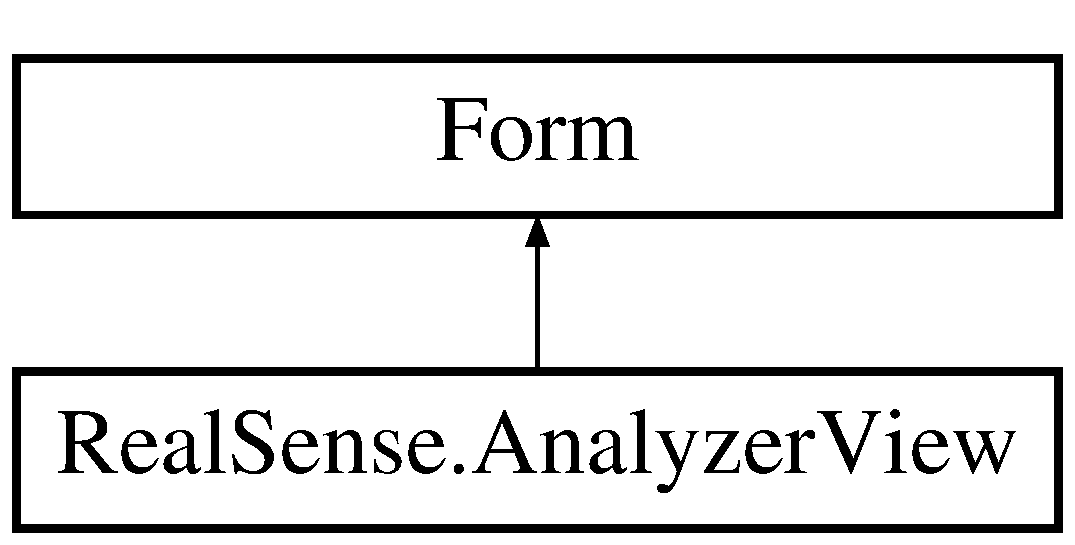
\includegraphics[height=2.000000cm]{class_real_sense_1_1_analyzer_view}
\end{center}
\end{figure}
\subsection*{Public Member Functions}
\begin{DoxyCompactItemize}
\item 
\textbf{ Analyzer\+View} ()
\end{DoxyCompactItemize}


\subsection{Detailed Description}
Sub-\/programm to revisit old landmark-\/recordings with updated algorithms to tweak the emotion-\/detection. Once the UI is loaded, the user can select on of the seven emotions and load their recorded data (both video-\/ and landmark-\/recordings). All of the landmark-\/recordings (recoding by recording, frame by frame) can then be used to automatically recalculate both the Action\+Unit-\/ and Emotiondata. This way, multiple subjects can be analyzed simultaneously and the reliability of the algorithms can be improved much faster. \begin{DoxyAuthor}{Author}
David  Hufflepuff 
\end{DoxyAuthor}


\subsection{Constructor \& Destructor Documentation}
\mbox{\label{class_real_sense_1_1_analyzer_view_ae982969308d52738e20d686cd24b88e8}} 
\index{Real\+Sense\+::\+Analyzer\+View@{Real\+Sense\+::\+Analyzer\+View}!Analyzer\+View@{Analyzer\+View}}
\index{Analyzer\+View@{Analyzer\+View}!Real\+Sense\+::\+Analyzer\+View@{Real\+Sense\+::\+Analyzer\+View}}
\subsubsection{Analyzer\+View()}
{\footnotesize\ttfamily Real\+Sense.\+Analyzer\+View.\+Analyzer\+View (\begin{DoxyParamCaption}{ }\end{DoxyParamCaption})}

Sets up the UI and starts the Updater-\/\+Thread, which will Update the lables and progressbars displaying the Action\+Unit-\/ and Emotion-\/\+Values 

The documentation for this class was generated from the following file\+:\begin{DoxyCompactItemize}
\item 
Analyse/\textbf{ Analyzer\+View.\+cs}\end{DoxyCompactItemize}

\hypertarget{class_real_sense_1_1_a_u___brow_shift}{}\section{Real\+Sense.\+A\+U\+\_\+\+Brow\+Shift Class Reference}
\label{class_real_sense_1_1_a_u___brow_shift}\index{Real\+Sense.\+A\+U\+\_\+\+Brow\+Shift@{Real\+Sense.\+A\+U\+\_\+\+Brow\+Shift}}
Inheritance diagram for Real\+Sense.\+A\+U\+\_\+\+Brow\+Shift\+:\begin{figure}[H]
\begin{center}
\leavevmode
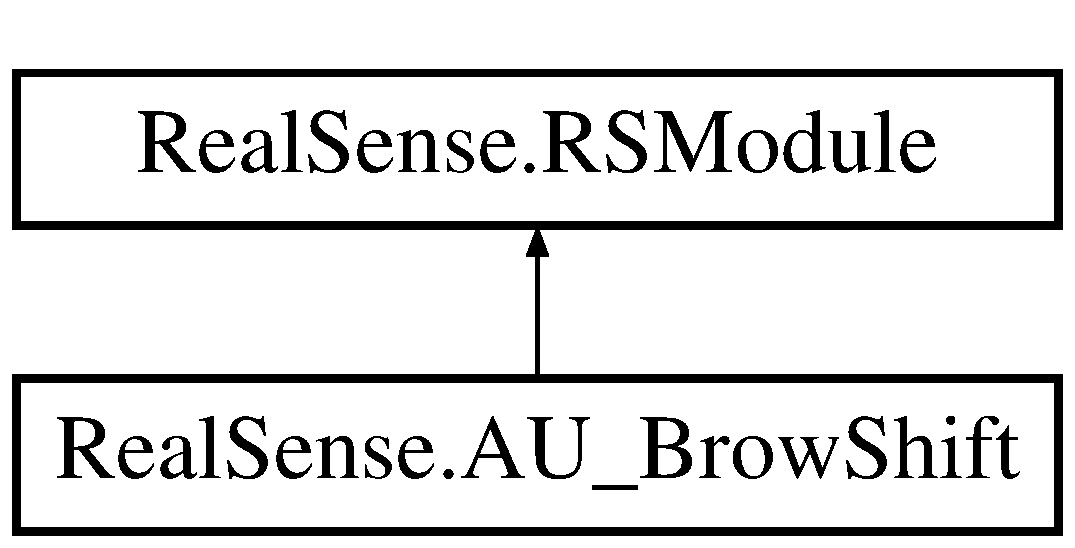
\includegraphics[height=2.000000cm]{class_real_sense_1_1_a_u___brow_shift}
\end{center}
\end{figure}
\subsection*{Public Member Functions}
\begin{DoxyCompactItemize}
\item 
\hyperlink{class_real_sense_1_1_a_u___brow_shift_a65b13018204e75f590f8422b0436e944}{A\+U\+\_\+\+Brow\+Shift} ()
\item 
override void \hyperlink{class_real_sense_1_1_a_u___brow_shift_a81ed7b844c217d3092412e0f53378dd5}{Work} (Graphics g)
\end{DoxyCompactItemize}
\subsection*{Additional Inherited Members}


\subsection{Detailed Description}


Definition at line 18 of file A\+U\+\_\+\+Brow\+Shift.\+cs.



\subsection{Constructor \& Destructor Documentation}
\mbox{\Hypertarget{class_real_sense_1_1_a_u___brow_shift_a65b13018204e75f590f8422b0436e944}\label{class_real_sense_1_1_a_u___brow_shift_a65b13018204e75f590f8422b0436e944}} 
\index{Real\+Sense\+::\+A\+U\+\_\+\+Brow\+Shift@{Real\+Sense\+::\+A\+U\+\_\+\+Brow\+Shift}!A\+U\+\_\+\+Brow\+Shift@{A\+U\+\_\+\+Brow\+Shift}}
\index{A\+U\+\_\+\+Brow\+Shift@{A\+U\+\_\+\+Brow\+Shift}!Real\+Sense\+::\+A\+U\+\_\+\+Brow\+Shift@{Real\+Sense\+::\+A\+U\+\_\+\+Brow\+Shift}}
\subsubsection{\texorpdfstring{A\+U\+\_\+\+Brow\+Shift()}{AU\_BrowShift()}}
{\footnotesize\ttfamily Real\+Sense.\+A\+U\+\_\+\+Brow\+Shift.\+A\+U\+\_\+\+Brow\+Shift (\begin{DoxyParamCaption}{ }\end{DoxyParamCaption})}

Initializes the AU by setting up the default value boundaries. 

Definition at line 29 of file A\+U\+\_\+\+Brow\+Shift.\+cs.



\subsection{Member Function Documentation}
\mbox{\Hypertarget{class_real_sense_1_1_a_u___brow_shift_a81ed7b844c217d3092412e0f53378dd5}\label{class_real_sense_1_1_a_u___brow_shift_a81ed7b844c217d3092412e0f53378dd5}} 
\index{Real\+Sense\+::\+A\+U\+\_\+\+Brow\+Shift@{Real\+Sense\+::\+A\+U\+\_\+\+Brow\+Shift}!Work@{Work}}
\index{Work@{Work}!Real\+Sense\+::\+A\+U\+\_\+\+Brow\+Shift@{Real\+Sense\+::\+A\+U\+\_\+\+Brow\+Shift}}
\subsubsection{\texorpdfstring{Work()}{Work()}}
{\footnotesize\ttfamily override void Real\+Sense.\+A\+U\+\_\+\+Brow\+Shift.\+Work (\begin{DoxyParamCaption}\item[{Graphics}]{g }\end{DoxyParamCaption})\hspace{0.3cm}{\ttfamily [virtual]}}

Computes the percentage Value of Brow\+Shift in the current Frame over a set number of frames and prints its\textquotesingle{} debug-\/message to the \hyperlink{class_real_sense_1_1_camera_view}{Camera\+View} when debug is enabled. 
\begin{DoxyParams}{Parameters}
{\em Graphics} & g for the view \\
\hline
\end{DoxyParams}


Implements \hyperlink{class_real_sense_1_1_r_s_module_a2ec830b7932ee7c0077d473f81c73867}{Real\+Sense.\+R\+S\+Module}.



Definition at line 50 of file A\+U\+\_\+\+Brow\+Shift.\+cs.



The documentation for this class was generated from the following file\+:\begin{DoxyCompactItemize}
\item 
Action\+Units/\hyperlink{_a_u___brow_shift_8cs}{A\+U\+\_\+\+Brow\+Shift.\+cs}\end{DoxyCompactItemize}

\hypertarget{class_real_sense_1_1_a_u___eyelid_tight}{}\section{Real\+Sense.\+A\+U\+\_\+\+Eyelid\+Tight Class Reference}
\label{class_real_sense_1_1_a_u___eyelid_tight}\index{Real\+Sense.\+A\+U\+\_\+\+Eyelid\+Tight@{Real\+Sense.\+A\+U\+\_\+\+Eyelid\+Tight}}
Inheritance diagram for Real\+Sense.\+A\+U\+\_\+\+Eyelid\+Tight\+:\begin{figure}[H]
\begin{center}
\leavevmode
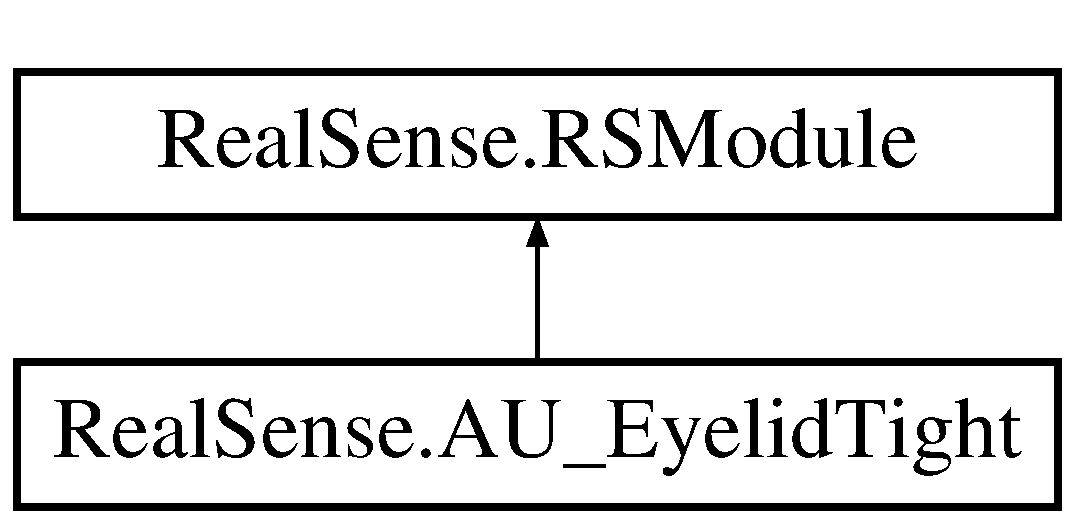
\includegraphics[height=2.000000cm]{class_real_sense_1_1_a_u___eyelid_tight}
\end{center}
\end{figure}
\subsection*{Public Member Functions}
\begin{DoxyCompactItemize}
\item 
\hyperlink{class_real_sense_1_1_a_u___eyelid_tight_a43f0e6e9a4e0862ae2044be31855df0b}{A\+U\+\_\+\+Eyelid\+Tight} ()
\item 
override void \hyperlink{class_real_sense_1_1_a_u___eyelid_tight_a778e09bf84946d959dcf3375a3c8d662}{Work} (Graphics g)
\end{DoxyCompactItemize}
\subsection*{Additional Inherited Members}


\subsection{Detailed Description}
Measures tightening of eyelids (each eye) and stores its\textquotesingle{} value inside the model. \begin{DoxyAuthor}{Author}
\+: David Rosenbusch  Hufflepuff
\end{DoxyAuthor}
Interpretation\+: -\/100 = Eyes squinted 100 = Eyes wide open 

Definition at line 19 of file A\+U\+\_\+\+Eyelid\+Tight.\+cs.



\subsection{Constructor \& Destructor Documentation}
\mbox{\Hypertarget{class_real_sense_1_1_a_u___eyelid_tight_a43f0e6e9a4e0862ae2044be31855df0b}\label{class_real_sense_1_1_a_u___eyelid_tight_a43f0e6e9a4e0862ae2044be31855df0b}} 
\index{Real\+Sense\+::\+A\+U\+\_\+\+Eyelid\+Tight@{Real\+Sense\+::\+A\+U\+\_\+\+Eyelid\+Tight}!A\+U\+\_\+\+Eyelid\+Tight@{A\+U\+\_\+\+Eyelid\+Tight}}
\index{A\+U\+\_\+\+Eyelid\+Tight@{A\+U\+\_\+\+Eyelid\+Tight}!Real\+Sense\+::\+A\+U\+\_\+\+Eyelid\+Tight@{Real\+Sense\+::\+A\+U\+\_\+\+Eyelid\+Tight}}
\subsubsection{\texorpdfstring{A\+U\+\_\+\+Eyelid\+Tight()}{AU\_EyelidTight()}}
{\footnotesize\ttfamily Real\+Sense.\+A\+U\+\_\+\+Eyelid\+Tight.\+A\+U\+\_\+\+Eyelid\+Tight (\begin{DoxyParamCaption}{ }\end{DoxyParamCaption})}

Initializes the AU by setting up the default value boundaries. 

Definition at line 32 of file A\+U\+\_\+\+Eyelid\+Tight.\+cs.



\subsection{Member Function Documentation}
\mbox{\Hypertarget{class_real_sense_1_1_a_u___eyelid_tight_a778e09bf84946d959dcf3375a3c8d662}\label{class_real_sense_1_1_a_u___eyelid_tight_a778e09bf84946d959dcf3375a3c8d662}} 
\index{Real\+Sense\+::\+A\+U\+\_\+\+Eyelid\+Tight@{Real\+Sense\+::\+A\+U\+\_\+\+Eyelid\+Tight}!Work@{Work}}
\index{Work@{Work}!Real\+Sense\+::\+A\+U\+\_\+\+Eyelid\+Tight@{Real\+Sense\+::\+A\+U\+\_\+\+Eyelid\+Tight}}
\subsubsection{\texorpdfstring{Work()}{Work()}}
{\footnotesize\ttfamily override void Real\+Sense.\+A\+U\+\_\+\+Eyelid\+Tight.\+Work (\begin{DoxyParamCaption}\item[{Graphics}]{g }\end{DoxyParamCaption})\hspace{0.3cm}{\ttfamily [virtual]}}

Calculates difference of lid-\/distance for each eye over a set number of frames and prints its\textquotesingle{} debug-\/message to the \hyperlink{class_real_sense_1_1_camera_view}{Camera\+View} when debug is enabled. 
\begin{DoxyParams}{Parameters}
{\em Graphics} & g for the view \\
\hline
\end{DoxyParams}


Implements \hyperlink{class_real_sense_1_1_r_s_module_a2ec830b7932ee7c0077d473f81c73867}{Real\+Sense.\+R\+S\+Module}.



Definition at line 56 of file A\+U\+\_\+\+Eyelid\+Tight.\+cs.



The documentation for this class was generated from the following file\+:\begin{DoxyCompactItemize}
\item 
Action\+Units/\hyperlink{_a_u___eyelid_tight_8cs}{A\+U\+\_\+\+Eyelid\+Tight.\+cs}\end{DoxyCompactItemize}

\section{Real\+Sense.\+A\+U\+\_\+\+Jaw\+Drop Class Reference}
\label{class_real_sense_1_1_a_u___jaw_drop}\index{Real\+Sense.\+A\+U\+\_\+\+Jaw\+Drop@{Real\+Sense.\+A\+U\+\_\+\+Jaw\+Drop}}
Inheritance diagram for Real\+Sense.\+A\+U\+\_\+\+Jaw\+Drop\+:\begin{figure}[H]
\begin{center}
\leavevmode
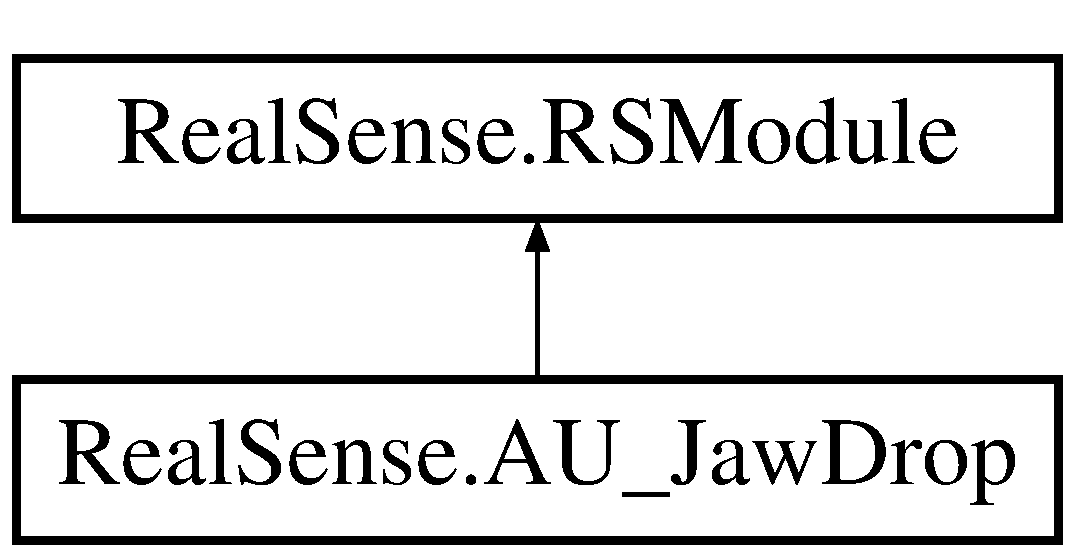
\includegraphics[height=2.000000cm]{class_real_sense_1_1_a_u___jaw_drop}
\end{center}
\end{figure}
\subsection*{Public Member Functions}
\begin{DoxyCompactItemize}
\item 
\textbf{ A\+U\+\_\+\+Jaw\+Drop} ()
\item 
override void \textbf{ Work} (Graphics g)
\end{DoxyCompactItemize}
\subsection*{Additional Inherited Members}


\subsection{Detailed Description}
Measures if jaw is dropped and stores its\textquotesingle{} value inside the model. \begin{DoxyAuthor}{Author}
René  Slytherin
\end{DoxyAuthor}
Interpretation\+: -\/100 = Doesn\textquotesingle{}t usually happen 0 = Normal 100 = Drop it like it\textquotesingle{}s hot 

\subsection{Constructor \& Destructor Documentation}
\mbox{\label{class_real_sense_1_1_a_u___jaw_drop_a28f51c63dfbf79d8315c689b6ae2b65b}} 
\index{Real\+Sense\+::\+A\+U\+\_\+\+Jaw\+Drop@{Real\+Sense\+::\+A\+U\+\_\+\+Jaw\+Drop}!A\+U\+\_\+\+Jaw\+Drop@{A\+U\+\_\+\+Jaw\+Drop}}
\index{A\+U\+\_\+\+Jaw\+Drop@{A\+U\+\_\+\+Jaw\+Drop}!Real\+Sense\+::\+A\+U\+\_\+\+Jaw\+Drop@{Real\+Sense\+::\+A\+U\+\_\+\+Jaw\+Drop}}
\subsubsection{A\+U\+\_\+\+Jaw\+Drop()}
{\footnotesize\ttfamily Real\+Sense.\+A\+U\+\_\+\+Jaw\+Drop.\+A\+U\+\_\+\+Jaw\+Drop (\begin{DoxyParamCaption}{ }\end{DoxyParamCaption})}

Initializes the AU by setting up the default value boundaries. 

\subsection{Member Function Documentation}
\mbox{\label{class_real_sense_1_1_a_u___jaw_drop_aed90ca88a1c563016c6af39fd65f81e4}} 
\index{Real\+Sense\+::\+A\+U\+\_\+\+Jaw\+Drop@{Real\+Sense\+::\+A\+U\+\_\+\+Jaw\+Drop}!Work@{Work}}
\index{Work@{Work}!Real\+Sense\+::\+A\+U\+\_\+\+Jaw\+Drop@{Real\+Sense\+::\+A\+U\+\_\+\+Jaw\+Drop}}
\subsubsection{Work()}
{\footnotesize\ttfamily override void Real\+Sense.\+A\+U\+\_\+\+Jaw\+Drop.\+Work (\begin{DoxyParamCaption}\item[{Graphics}]{g }\end{DoxyParamCaption})\hspace{0.3cm}{\ttfamily [virtual]}}

Calculates difference of lip-\/distance over a set number of frames and prints its\textquotesingle{} debug-\/message to the \doxyref{Camera\+View}{p.}{class_real_sense_1_1_camera_view} when debug is enabled. 
\begin{DoxyParams}{Parameters}
{\em Graphics} & g for the view \\
\hline
\end{DoxyParams}


Implements \textbf{ Real\+Sense.\+R\+S\+Module} \doxyref{}{p.}{class_real_sense_1_1_r_s_module_a2ec830b7932ee7c0077d473f81c73867}.



The documentation for this class was generated from the following file\+:\begin{DoxyCompactItemize}
\item 
Action\+Units/\textbf{ A\+U\+\_\+\+Jaw\+Drop.\+cs}\end{DoxyCompactItemize}

\hypertarget{class_real_sense_1_1_a_u___lip_corner}{}\section{Real\+Sense.\+A\+U\+\_\+\+Lip\+Corner Class Reference}
\label{class_real_sense_1_1_a_u___lip_corner}\index{Real\+Sense.\+A\+U\+\_\+\+Lip\+Corner@{Real\+Sense.\+A\+U\+\_\+\+Lip\+Corner}}
Inheritance diagram for Real\+Sense.\+A\+U\+\_\+\+Lip\+Corner\+:\begin{figure}[H]
\begin{center}
\leavevmode
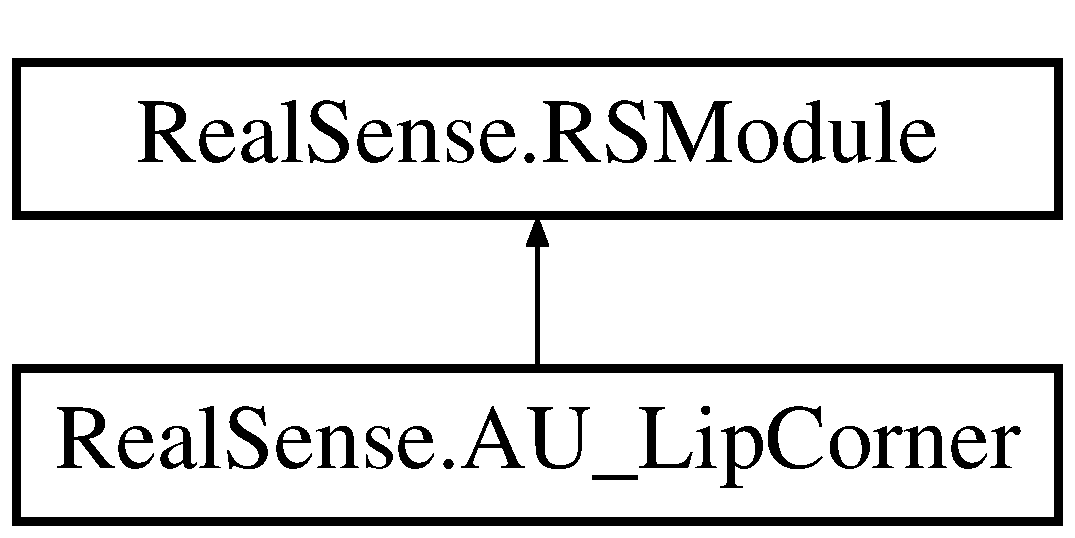
\includegraphics[height=2.000000cm]{class_real_sense_1_1_a_u___lip_corner}
\end{center}
\end{figure}
\subsection*{Public Member Functions}
\begin{DoxyCompactItemize}
\item 
\hyperlink{class_real_sense_1_1_a_u___lip_corner_ae3bb4bd3aad86a0c83d5bc57b9bb0855}{A\+U\+\_\+\+Lip\+Corner} ()
\item 
override void \hyperlink{class_real_sense_1_1_a_u___lip_corner_a4a506c5dc50e7bcd8dcfa80cecbd7f56}{Work} (Graphics g)
\end{DoxyCompactItemize}
\subsection*{Additional Inherited Members}


\subsection{Detailed Description}
Measures the height of the Lip-\/\+Corners and stores its\textquotesingle{} value inside the model. \begin{DoxyAuthor}{Author}
Marlon  Hufflepuff
\end{DoxyAuthor}
Interpretation\+: -\/100 = Corners down (not reliable, use Lip\+Line) set to 0! 100 = Big stupid smile 

Definition at line 19 of file A\+U\+\_\+\+Lip\+Corner.\+cs.



\subsection{Constructor \& Destructor Documentation}
\mbox{\Hypertarget{class_real_sense_1_1_a_u___lip_corner_ae3bb4bd3aad86a0c83d5bc57b9bb0855}\label{class_real_sense_1_1_a_u___lip_corner_ae3bb4bd3aad86a0c83d5bc57b9bb0855}} 
\index{Real\+Sense\+::\+A\+U\+\_\+\+Lip\+Corner@{Real\+Sense\+::\+A\+U\+\_\+\+Lip\+Corner}!A\+U\+\_\+\+Lip\+Corner@{A\+U\+\_\+\+Lip\+Corner}}
\index{A\+U\+\_\+\+Lip\+Corner@{A\+U\+\_\+\+Lip\+Corner}!Real\+Sense\+::\+A\+U\+\_\+\+Lip\+Corner@{Real\+Sense\+::\+A\+U\+\_\+\+Lip\+Corner}}
\subsubsection{\texorpdfstring{A\+U\+\_\+\+Lip\+Corner()}{AU\_LipCorner()}}
{\footnotesize\ttfamily Real\+Sense.\+A\+U\+\_\+\+Lip\+Corner.\+A\+U\+\_\+\+Lip\+Corner (\begin{DoxyParamCaption}{ }\end{DoxyParamCaption})}

Initializes the AU by setting up the default value boundaries. 

Definition at line 30 of file A\+U\+\_\+\+Lip\+Corner.\+cs.



\subsection{Member Function Documentation}
\mbox{\Hypertarget{class_real_sense_1_1_a_u___lip_corner_a4a506c5dc50e7bcd8dcfa80cecbd7f56}\label{class_real_sense_1_1_a_u___lip_corner_a4a506c5dc50e7bcd8dcfa80cecbd7f56}} 
\index{Real\+Sense\+::\+A\+U\+\_\+\+Lip\+Corner@{Real\+Sense\+::\+A\+U\+\_\+\+Lip\+Corner}!Work@{Work}}
\index{Work@{Work}!Real\+Sense\+::\+A\+U\+\_\+\+Lip\+Corner@{Real\+Sense\+::\+A\+U\+\_\+\+Lip\+Corner}}
\subsubsection{\texorpdfstring{Work()}{Work()}}
{\footnotesize\ttfamily override void Real\+Sense.\+A\+U\+\_\+\+Lip\+Corner.\+Work (\begin{DoxyParamCaption}\item[{Graphics}]{g }\end{DoxyParamCaption})\hspace{0.3cm}{\ttfamily [virtual]}}

Calculates the height of the Lipcorners over a set number of frames and prints its\textquotesingle{} debug-\/message to the \hyperlink{class_real_sense_1_1_camera_view}{Camera\+View} when debug is enabled. 
\begin{DoxyParams}{Parameters}
{\em Graphics} & g for the view \\
\hline
\end{DoxyParams}


Implements \hyperlink{class_real_sense_1_1_r_s_module_a2ec830b7932ee7c0077d473f81c73867}{Real\+Sense.\+R\+S\+Module}.



Definition at line 49 of file A\+U\+\_\+\+Lip\+Corner.\+cs.



The documentation for this class was generated from the following file\+:\begin{DoxyCompactItemize}
\item 
C\+:/\+Users/nutzer/\+Documents/\+Git\+Hub/\+Real\+Sense/\+Action\+Units/\hyperlink{_a_u___lip_corner_8cs}{A\+U\+\_\+\+Lip\+Corner.\+cs}\end{DoxyCompactItemize}

\hypertarget{class_real_sense_1_1_a_u___lip_line}{}\section{Real\+Sense.\+A\+U\+\_\+\+Lip\+Line Class Reference}
\label{class_real_sense_1_1_a_u___lip_line}\index{Real\+Sense.\+A\+U\+\_\+\+Lip\+Line@{Real\+Sense.\+A\+U\+\_\+\+Lip\+Line}}
Inheritance diagram for Real\+Sense.\+A\+U\+\_\+\+Lip\+Line\+:\begin{figure}[H]
\begin{center}
\leavevmode
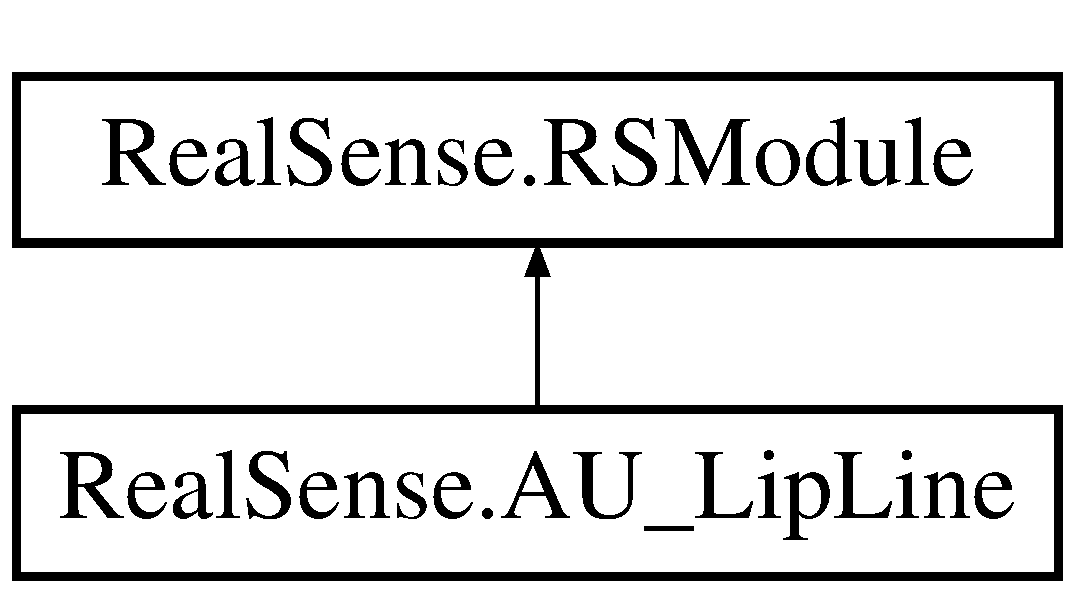
\includegraphics[height=2.000000cm]{class_real_sense_1_1_a_u___lip_line}
\end{center}
\end{figure}
\subsection*{Public Member Functions}
\begin{DoxyCompactItemize}
\item 
\hyperlink{class_real_sense_1_1_a_u___lip_line_a3059aba79e0a4aee393f31503675355f}{A\+U\+\_\+\+Lip\+Line} ()
\item 
override void \hyperlink{class_real_sense_1_1_a_u___lip_line_ac511da241ef7448f552111e3c5365de1}{Work} (Graphics g)
\end{DoxyCompactItemize}
\subsection*{Additional Inherited Members}


\subsection{Detailed Description}


Definition at line 19 of file A\+U\+\_\+\+Lip\+Line.\+cs.



\subsection{Constructor \& Destructor Documentation}
\mbox{\Hypertarget{class_real_sense_1_1_a_u___lip_line_a3059aba79e0a4aee393f31503675355f}\label{class_real_sense_1_1_a_u___lip_line_a3059aba79e0a4aee393f31503675355f}} 
\index{Real\+Sense\+::\+A\+U\+\_\+\+Lip\+Line@{Real\+Sense\+::\+A\+U\+\_\+\+Lip\+Line}!A\+U\+\_\+\+Lip\+Line@{A\+U\+\_\+\+Lip\+Line}}
\index{A\+U\+\_\+\+Lip\+Line@{A\+U\+\_\+\+Lip\+Line}!Real\+Sense\+::\+A\+U\+\_\+\+Lip\+Line@{Real\+Sense\+::\+A\+U\+\_\+\+Lip\+Line}}
\subsubsection{\texorpdfstring{A\+U\+\_\+\+Lip\+Line()}{AU\_LipLine()}}
{\footnotesize\ttfamily Real\+Sense.\+A\+U\+\_\+\+Lip\+Line.\+A\+U\+\_\+\+Lip\+Line (\begin{DoxyParamCaption}{ }\end{DoxyParamCaption})}

Initializes the AU by setting up the default value boundaries. 

Definition at line 28 of file A\+U\+\_\+\+Lip\+Line.\+cs.



\subsection{Member Function Documentation}
\mbox{\Hypertarget{class_real_sense_1_1_a_u___lip_line_ac511da241ef7448f552111e3c5365de1}\label{class_real_sense_1_1_a_u___lip_line_ac511da241ef7448f552111e3c5365de1}} 
\index{Real\+Sense\+::\+A\+U\+\_\+\+Lip\+Line@{Real\+Sense\+::\+A\+U\+\_\+\+Lip\+Line}!Work@{Work}}
\index{Work@{Work}!Real\+Sense\+::\+A\+U\+\_\+\+Lip\+Line@{Real\+Sense\+::\+A\+U\+\_\+\+Lip\+Line}}
\subsubsection{\texorpdfstring{Work()}{Work()}}
{\footnotesize\ttfamily override void Real\+Sense.\+A\+U\+\_\+\+Lip\+Line.\+Work (\begin{DoxyParamCaption}\item[{Graphics}]{g }\end{DoxyParamCaption})\hspace{0.3cm}{\ttfamily [virtual]}}

Calculates whether or not all Lip\+Points are placed on one line over a set number of frames and prints its\textquotesingle{} debug-\/message to the \hyperlink{class_real_sense_1_1_camera_view}{Camera\+View} when debug is enabled. 
\begin{DoxyParams}{Parameters}
{\em Graphics} & g for the view \\
\hline
\end{DoxyParams}


Implements \hyperlink{class_real_sense_1_1_r_s_module_a2ec830b7932ee7c0077d473f81c73867}{Real\+Sense.\+R\+S\+Module}.



Definition at line 46 of file A\+U\+\_\+\+Lip\+Line.\+cs.



The documentation for this class was generated from the following file\+:\begin{DoxyCompactItemize}
\item 
Action\+Units/\hyperlink{_a_u___lip_line_8cs}{A\+U\+\_\+\+Lip\+Line.\+cs}\end{DoxyCompactItemize}

\hypertarget{class_real_sense_1_1_a_u___lips_tightened}{}\section{Real\+Sense.\+A\+U\+\_\+\+Lips\+Tightened Class Reference}
\label{class_real_sense_1_1_a_u___lips_tightened}\index{Real\+Sense.\+A\+U\+\_\+\+Lips\+Tightened@{Real\+Sense.\+A\+U\+\_\+\+Lips\+Tightened}}
Inheritance diagram for Real\+Sense.\+A\+U\+\_\+\+Lips\+Tightened\+:\begin{figure}[H]
\begin{center}
\leavevmode
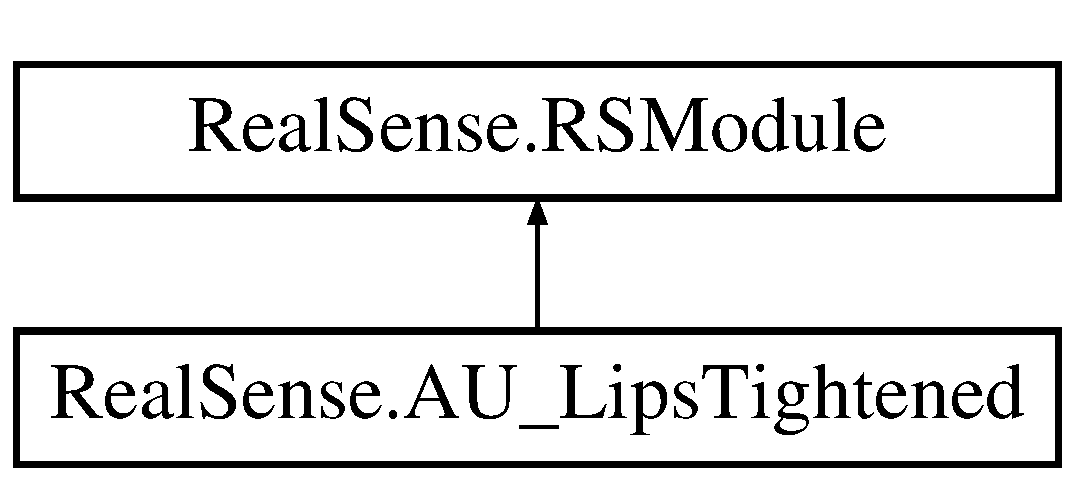
\includegraphics[height=2.000000cm]{class_real_sense_1_1_a_u___lips_tightened}
\end{center}
\end{figure}
\subsection*{Public Member Functions}
\begin{DoxyCompactItemize}
\item 
\hyperlink{class_real_sense_1_1_a_u___lips_tightened_abcb4ab60b321ea1e7edf7f1521aa30de}{A\+U\+\_\+\+Lips\+Tightened} ()
\item 
override void \hyperlink{class_real_sense_1_1_a_u___lips_tightened_a409b75e75c7b72c628ea6479a50ed75f}{Work} (Graphics g)
\end{DoxyCompactItemize}
\subsection*{Additional Inherited Members}


\subsection{Detailed Description}
Measures if lips are tightened and stores its\textquotesingle{} value inside the model. \begin{DoxyAuthor}{Author}
René  Slytherin
\end{DoxyAuthor}
Interpretation\+: -\/100 = Tight af 0 = normal 100 = doesn\textquotesingle{}t usually happen 

Definition at line 19 of file A\+U\+\_\+\+Lips\+Tightened.\+cs.



\subsection{Constructor \& Destructor Documentation}
\mbox{\Hypertarget{class_real_sense_1_1_a_u___lips_tightened_abcb4ab60b321ea1e7edf7f1521aa30de}\label{class_real_sense_1_1_a_u___lips_tightened_abcb4ab60b321ea1e7edf7f1521aa30de}} 
\index{Real\+Sense\+::\+A\+U\+\_\+\+Lips\+Tightened@{Real\+Sense\+::\+A\+U\+\_\+\+Lips\+Tightened}!A\+U\+\_\+\+Lips\+Tightened@{A\+U\+\_\+\+Lips\+Tightened}}
\index{A\+U\+\_\+\+Lips\+Tightened@{A\+U\+\_\+\+Lips\+Tightened}!Real\+Sense\+::\+A\+U\+\_\+\+Lips\+Tightened@{Real\+Sense\+::\+A\+U\+\_\+\+Lips\+Tightened}}
\subsubsection{\texorpdfstring{A\+U\+\_\+\+Lips\+Tightened()}{AU\_LipsTightened()}}
{\footnotesize\ttfamily Real\+Sense.\+A\+U\+\_\+\+Lips\+Tightened.\+A\+U\+\_\+\+Lips\+Tightened (\begin{DoxyParamCaption}{ }\end{DoxyParamCaption})}

Initializes the AU by setting up the default value boundaries. 

Definition at line 29 of file A\+U\+\_\+\+Lips\+Tightened.\+cs.



\subsection{Member Function Documentation}
\mbox{\Hypertarget{class_real_sense_1_1_a_u___lips_tightened_a409b75e75c7b72c628ea6479a50ed75f}\label{class_real_sense_1_1_a_u___lips_tightened_a409b75e75c7b72c628ea6479a50ed75f}} 
\index{Real\+Sense\+::\+A\+U\+\_\+\+Lips\+Tightened@{Real\+Sense\+::\+A\+U\+\_\+\+Lips\+Tightened}!Work@{Work}}
\index{Work@{Work}!Real\+Sense\+::\+A\+U\+\_\+\+Lips\+Tightened@{Real\+Sense\+::\+A\+U\+\_\+\+Lips\+Tightened}}
\subsubsection{\texorpdfstring{Work()}{Work()}}
{\footnotesize\ttfamily override void Real\+Sense.\+A\+U\+\_\+\+Lips\+Tightened.\+Work (\begin{DoxyParamCaption}\item[{Graphics}]{g }\end{DoxyParamCaption})\hspace{0.3cm}{\ttfamily [virtual]}}

Calculates the average difference of the lip and the nose over a set number of frames and prints its\textquotesingle{} debug-\/message to the \hyperlink{class_real_sense_1_1_camera_view}{Camera\+View} when debug is enabled. 
\begin{DoxyParams}{Parameters}
{\em Graphics} & g for the view \\
\hline
\end{DoxyParams}


Implements \hyperlink{class_real_sense_1_1_r_s_module_a2ec830b7932ee7c0077d473f81c73867}{Real\+Sense.\+R\+S\+Module}.



Definition at line 48 of file A\+U\+\_\+\+Lips\+Tightened.\+cs.



The documentation for this class was generated from the following file\+:\begin{DoxyCompactItemize}
\item 
C\+:/\+Users/nutzer/\+Documents/\+Git\+Hub/\+Real\+Sense/\+Action\+Units/\hyperlink{_a_u___lips_tightened_8cs}{A\+U\+\_\+\+Lips\+Tightened.\+cs}\end{DoxyCompactItemize}

\hypertarget{class_real_sense_1_1_a_u___lip_stretched}{}\section{Real\+Sense.\+A\+U\+\_\+\+Lip\+Stretched Class Reference}
\label{class_real_sense_1_1_a_u___lip_stretched}\index{Real\+Sense.\+A\+U\+\_\+\+Lip\+Stretched@{Real\+Sense.\+A\+U\+\_\+\+Lip\+Stretched}}
Inheritance diagram for Real\+Sense.\+A\+U\+\_\+\+Lip\+Stretched\+:\begin{figure}[H]
\begin{center}
\leavevmode
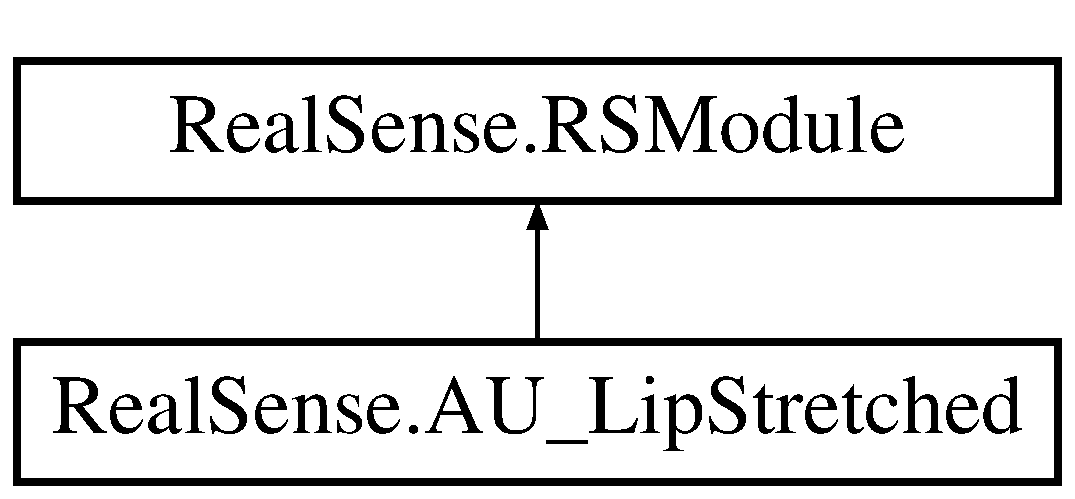
\includegraphics[height=2.000000cm]{class_real_sense_1_1_a_u___lip_stretched}
\end{center}
\end{figure}
\subsection*{Public Member Functions}
\begin{DoxyCompactItemize}
\item 
\hyperlink{class_real_sense_1_1_a_u___lip_stretched_aca5f1fcfb7f81dccdc700dfc025b4b39}{A\+U\+\_\+\+Lip\+Stretched} ()
\item 
override void \hyperlink{class_real_sense_1_1_a_u___lip_stretched_a2ec4542e5c8fa5585e66ee6ee44ab151}{Work} (Graphics g)
\end{DoxyCompactItemize}
\subsection*{Additional Inherited Members}


\subsection{Detailed Description}
Measures whether the lips are stretched and stores its\textquotesingle{} value inside the model. \begin{DoxyAuthor}{Author}
Tobias Schramm  Hufflepuff
\end{DoxyAuthor}
Interpretation\+: -\/100 = Kissing 0 = Relaxed 100 = Frogface 

Definition at line 19 of file A\+U\+\_\+\+Lip\+Stretched.\+cs.



\subsection{Constructor \& Destructor Documentation}
\mbox{\Hypertarget{class_real_sense_1_1_a_u___lip_stretched_aca5f1fcfb7f81dccdc700dfc025b4b39}\label{class_real_sense_1_1_a_u___lip_stretched_aca5f1fcfb7f81dccdc700dfc025b4b39}} 
\index{Real\+Sense\+::\+A\+U\+\_\+\+Lip\+Stretched@{Real\+Sense\+::\+A\+U\+\_\+\+Lip\+Stretched}!A\+U\+\_\+\+Lip\+Stretched@{A\+U\+\_\+\+Lip\+Stretched}}
\index{A\+U\+\_\+\+Lip\+Stretched@{A\+U\+\_\+\+Lip\+Stretched}!Real\+Sense\+::\+A\+U\+\_\+\+Lip\+Stretched@{Real\+Sense\+::\+A\+U\+\_\+\+Lip\+Stretched}}
\subsubsection{\texorpdfstring{A\+U\+\_\+\+Lip\+Stretched()}{AU\_LipStretched()}}
{\footnotesize\ttfamily Real\+Sense.\+A\+U\+\_\+\+Lip\+Stretched.\+A\+U\+\_\+\+Lip\+Stretched (\begin{DoxyParamCaption}{ }\end{DoxyParamCaption})}

Initializes the AU by setting up the default value boundaries. 

Definition at line 30 of file A\+U\+\_\+\+Lip\+Stretched.\+cs.



\subsection{Member Function Documentation}
\mbox{\Hypertarget{class_real_sense_1_1_a_u___lip_stretched_a2ec4542e5c8fa5585e66ee6ee44ab151}\label{class_real_sense_1_1_a_u___lip_stretched_a2ec4542e5c8fa5585e66ee6ee44ab151}} 
\index{Real\+Sense\+::\+A\+U\+\_\+\+Lip\+Stretched@{Real\+Sense\+::\+A\+U\+\_\+\+Lip\+Stretched}!Work@{Work}}
\index{Work@{Work}!Real\+Sense\+::\+A\+U\+\_\+\+Lip\+Stretched@{Real\+Sense\+::\+A\+U\+\_\+\+Lip\+Stretched}}
\subsubsection{\texorpdfstring{Work()}{Work()}}
{\footnotesize\ttfamily override void Real\+Sense.\+A\+U\+\_\+\+Lip\+Stretched.\+Work (\begin{DoxyParamCaption}\item[{Graphics}]{g }\end{DoxyParamCaption})\hspace{0.3cm}{\ttfamily [virtual]}}

Calculates the average difference between the two lip corners over a set number of frames and prints its\textquotesingle{} debug-\/message to the \hyperlink{class_real_sense_1_1_camera_view}{Camera\+View} when debug is enabled. 
\begin{DoxyParams}{Parameters}
{\em Graphics} & g for the view \\
\hline
\end{DoxyParams}


Implements \hyperlink{class_real_sense_1_1_r_s_module_a2ec830b7932ee7c0077d473f81c73867}{Real\+Sense.\+R\+S\+Module}.



Definition at line 48 of file A\+U\+\_\+\+Lip\+Stretched.\+cs.



The documentation for this class was generated from the following file\+:\begin{DoxyCompactItemize}
\item 
C\+:/\+Users/nutzer/\+Documents/\+Git\+Hub/\+Real\+Sense/\+Action\+Units/\hyperlink{_a_u___lip_stretched_8cs}{A\+U\+\_\+\+Lip\+Stretched.\+cs}\end{DoxyCompactItemize}

\section{Real\+Sense.\+A\+U\+\_\+\+Lower\+Lip\+Lowered Class Reference}
\label{class_real_sense_1_1_a_u___lower_lip_lowered}\index{Real\+Sense.\+A\+U\+\_\+\+Lower\+Lip\+Lowered@{Real\+Sense.\+A\+U\+\_\+\+Lower\+Lip\+Lowered}}
Inheritance diagram for Real\+Sense.\+A\+U\+\_\+\+Lower\+Lip\+Lowered\+:\begin{figure}[H]
\begin{center}
\leavevmode
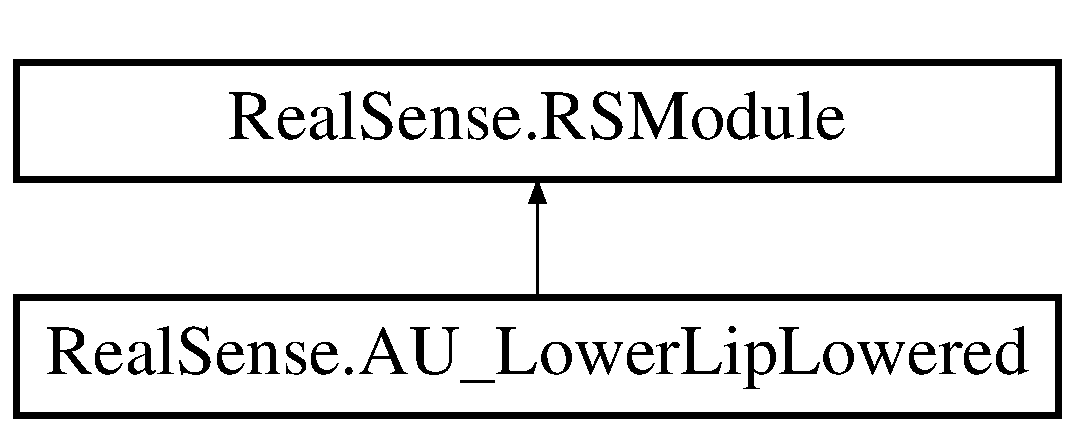
\includegraphics[height=2.000000cm]{class_real_sense_1_1_a_u___lower_lip_lowered}
\end{center}
\end{figure}
\subsection*{Public Member Functions}
\begin{DoxyCompactItemize}
\item 
\textbf{ A\+U\+\_\+\+Lower\+Lip\+Lowered} ()
\item 
override void \textbf{ Work} (Graphics g)
\end{DoxyCompactItemize}
\subsection*{Additional Inherited Members}


\subsection{Detailed Description}
Measures whether the lower lip is lower and stores its\textquotesingle{} value inside the model \begin{DoxyAuthor}{Author}
Tobias Schramm  Hufflepuff
\end{DoxyAuthor}
Interpretation\+: 0 = Relaxed 100 = Lip down 

\subsection{Constructor \& Destructor Documentation}
\mbox{\label{class_real_sense_1_1_a_u___lower_lip_lowered_a510ce477e2525d7859299aaf92c3c88b}} 
\index{Real\+Sense\+::\+A\+U\+\_\+\+Lower\+Lip\+Lowered@{Real\+Sense\+::\+A\+U\+\_\+\+Lower\+Lip\+Lowered}!A\+U\+\_\+\+Lower\+Lip\+Lowered@{A\+U\+\_\+\+Lower\+Lip\+Lowered}}
\index{A\+U\+\_\+\+Lower\+Lip\+Lowered@{A\+U\+\_\+\+Lower\+Lip\+Lowered}!Real\+Sense\+::\+A\+U\+\_\+\+Lower\+Lip\+Lowered@{Real\+Sense\+::\+A\+U\+\_\+\+Lower\+Lip\+Lowered}}
\subsubsection{A\+U\+\_\+\+Lower\+Lip\+Lowered()}
{\footnotesize\ttfamily Real\+Sense.\+A\+U\+\_\+\+Lower\+Lip\+Lowered.\+A\+U\+\_\+\+Lower\+Lip\+Lowered (\begin{DoxyParamCaption}{ }\end{DoxyParamCaption})}

Initializes the AU by setting up the default value boundaries. 

\subsection{Member Function Documentation}
\mbox{\label{class_real_sense_1_1_a_u___lower_lip_lowered_ad94e215984e23238a6231d6a9723a522}} 
\index{Real\+Sense\+::\+A\+U\+\_\+\+Lower\+Lip\+Lowered@{Real\+Sense\+::\+A\+U\+\_\+\+Lower\+Lip\+Lowered}!Work@{Work}}
\index{Work@{Work}!Real\+Sense\+::\+A\+U\+\_\+\+Lower\+Lip\+Lowered@{Real\+Sense\+::\+A\+U\+\_\+\+Lower\+Lip\+Lowered}}
\subsubsection{Work()}
{\footnotesize\ttfamily override void Real\+Sense.\+A\+U\+\_\+\+Lower\+Lip\+Lowered.\+Work (\begin{DoxyParamCaption}\item[{Graphics}]{g }\end{DoxyParamCaption})\hspace{0.3cm}{\ttfamily [virtual]}}

Calculates the average difference between the lower lip and the nose to see if the lower lip was moved over a set number of frames and prints its\textquotesingle{} debug-\/message to the \doxyref{Camera\+View}{p.}{class_real_sense_1_1_camera_view} when debug is enabled. 
\begin{DoxyParams}{Parameters}
{\em Graphics} & g for the view \\
\hline
\end{DoxyParams}


Implements \textbf{ Real\+Sense.\+R\+S\+Module} \doxyref{}{p.}{class_real_sense_1_1_r_s_module_a2ec830b7932ee7c0077d473f81c73867}.



The documentation for this class was generated from the following file\+:\begin{DoxyCompactItemize}
\item 
Action\+Units/\textbf{ A\+U\+\_\+\+Lower\+Lip\+Lowered.\+cs}\end{DoxyCompactItemize}

\hypertarget{class_real_sense_1_1_a_u___lower_lip_raised}{}\section{Real\+Sense.\+A\+U\+\_\+\+Lower\+Lip\+Raised Class Reference}
\label{class_real_sense_1_1_a_u___lower_lip_raised}\index{Real\+Sense.\+A\+U\+\_\+\+Lower\+Lip\+Raised@{Real\+Sense.\+A\+U\+\_\+\+Lower\+Lip\+Raised}}
Inheritance diagram for Real\+Sense.\+A\+U\+\_\+\+Lower\+Lip\+Raised\+:\begin{figure}[H]
\begin{center}
\leavevmode
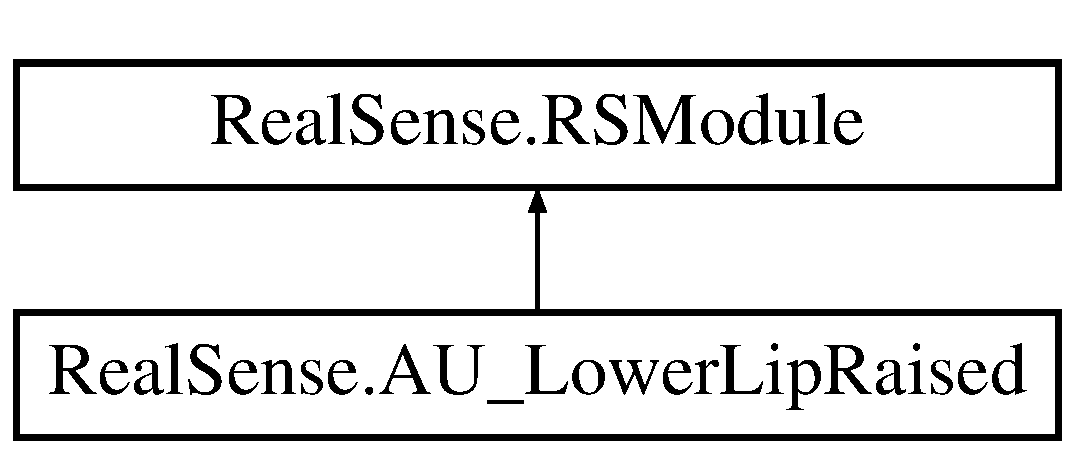
\includegraphics[height=2.000000cm]{class_real_sense_1_1_a_u___lower_lip_raised}
\end{center}
\end{figure}
\subsection*{Public Member Functions}
\begin{DoxyCompactItemize}
\item 
\hyperlink{class_real_sense_1_1_a_u___lower_lip_raised_aae4c2bb8b4a75fcfc59867f1950f823a}{A\+U\+\_\+\+Lower\+Lip\+Raised} ()
\item 
override void \hyperlink{class_real_sense_1_1_a_u___lower_lip_raised_aa3949d4b7a3adf5d38cb5ad5acd5c8f2}{Work} (Graphics g)
\end{DoxyCompactItemize}
\subsection*{Additional Inherited Members}


\subsection{Detailed Description}
Measures how much the lower lip is raised and stores its\textquotesingle{} value inside the model. \begin{DoxyAuthor}{Author}
\+: He who must not be named...  Take a guess...
\end{DoxyAuthor}
Interpretation\+: 0 = Relaxed -\/100 = Wrinkled 

Definition at line 17 of file A\+U\+\_\+\+Lower\+Lip\+Raised.\+cs.



\subsection{Constructor \& Destructor Documentation}
\mbox{\Hypertarget{class_real_sense_1_1_a_u___lower_lip_raised_aae4c2bb8b4a75fcfc59867f1950f823a}\label{class_real_sense_1_1_a_u___lower_lip_raised_aae4c2bb8b4a75fcfc59867f1950f823a}} 
\index{Real\+Sense\+::\+A\+U\+\_\+\+Lower\+Lip\+Raised@{Real\+Sense\+::\+A\+U\+\_\+\+Lower\+Lip\+Raised}!A\+U\+\_\+\+Lower\+Lip\+Raised@{A\+U\+\_\+\+Lower\+Lip\+Raised}}
\index{A\+U\+\_\+\+Lower\+Lip\+Raised@{A\+U\+\_\+\+Lower\+Lip\+Raised}!Real\+Sense\+::\+A\+U\+\_\+\+Lower\+Lip\+Raised@{Real\+Sense\+::\+A\+U\+\_\+\+Lower\+Lip\+Raised}}
\subsubsection{\texorpdfstring{A\+U\+\_\+\+Lower\+Lip\+Raised()}{AU\_LowerLipRaised()}}
{\footnotesize\ttfamily Real\+Sense.\+A\+U\+\_\+\+Lower\+Lip\+Raised.\+A\+U\+\_\+\+Lower\+Lip\+Raised (\begin{DoxyParamCaption}{ }\end{DoxyParamCaption})}

Initializes the AU by setting up the default value boundaries. 

Definition at line 28 of file A\+U\+\_\+\+Lower\+Lip\+Raised.\+cs.



\subsection{Member Function Documentation}
\mbox{\Hypertarget{class_real_sense_1_1_a_u___lower_lip_raised_aa3949d4b7a3adf5d38cb5ad5acd5c8f2}\label{class_real_sense_1_1_a_u___lower_lip_raised_aa3949d4b7a3adf5d38cb5ad5acd5c8f2}} 
\index{Real\+Sense\+::\+A\+U\+\_\+\+Lower\+Lip\+Raised@{Real\+Sense\+::\+A\+U\+\_\+\+Lower\+Lip\+Raised}!Work@{Work}}
\index{Work@{Work}!Real\+Sense\+::\+A\+U\+\_\+\+Lower\+Lip\+Raised@{Real\+Sense\+::\+A\+U\+\_\+\+Lower\+Lip\+Raised}}
\subsubsection{\texorpdfstring{Work()}{Work()}}
{\footnotesize\ttfamily override void Real\+Sense.\+A\+U\+\_\+\+Lower\+Lip\+Raised.\+Work (\begin{DoxyParamCaption}\item[{Graphics}]{g }\end{DoxyParamCaption})\hspace{0.3cm}{\ttfamily [virtual]}}

Calculates the difference between the lower lip and the nose to measure whether or not there has been some movement over a set number of frames and prints its\textquotesingle{} debug-\/message to the \hyperlink{class_real_sense_1_1_camera_view}{Camera\+View} when debug is enabled. 
\begin{DoxyParams}{Parameters}
{\em Graphics} & g for the view \\
\hline
\end{DoxyParams}


Implements \hyperlink{class_real_sense_1_1_r_s_module_a2ec830b7932ee7c0077d473f81c73867}{Real\+Sense.\+R\+S\+Module}.



Definition at line 46 of file A\+U\+\_\+\+Lower\+Lip\+Raised.\+cs.



The documentation for this class was generated from the following file\+:\begin{DoxyCompactItemize}
\item 
C\+:/\+Users/nutzer/\+Documents/\+Git\+Hub/\+Real\+Sense/\+Action\+Units/\hyperlink{_a_u___lower_lip_raised_8cs}{A\+U\+\_\+\+Lower\+Lip\+Raised.\+cs}\end{DoxyCompactItemize}

\hypertarget{class_real_sense_1_1_a_u___nose_wrinkled}{}\section{Real\+Sense.\+A\+U\+\_\+\+Nose\+Wrinkled Class Reference}
\label{class_real_sense_1_1_a_u___nose_wrinkled}\index{Real\+Sense.\+A\+U\+\_\+\+Nose\+Wrinkled@{Real\+Sense.\+A\+U\+\_\+\+Nose\+Wrinkled}}
Inheritance diagram for Real\+Sense.\+A\+U\+\_\+\+Nose\+Wrinkled\+:\begin{figure}[H]
\begin{center}
\leavevmode
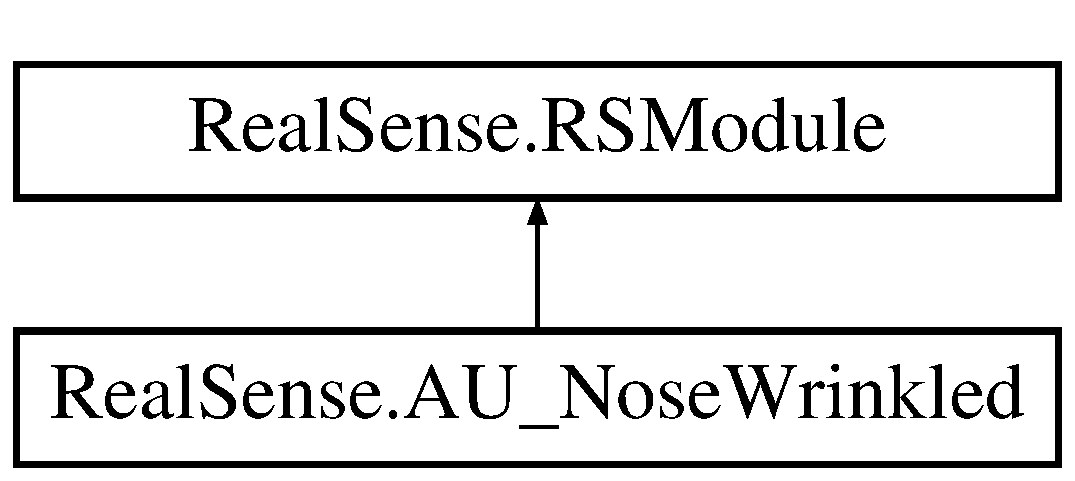
\includegraphics[height=2.000000cm]{class_real_sense_1_1_a_u___nose_wrinkled}
\end{center}
\end{figure}
\subsection*{Public Member Functions}
\begin{DoxyCompactItemize}
\item 
\hyperlink{class_real_sense_1_1_a_u___nose_wrinkled_a1dfdf22628e88a848b5359e623294044}{A\+U\+\_\+\+Nose\+Wrinkled} ()
\item 
override void \hyperlink{class_real_sense_1_1_a_u___nose_wrinkled_afa5099e1c15f8f0f3d9633a42ed69817}{Work} (Graphics g)
\end{DoxyCompactItemize}
\subsection*{Additional Inherited Members}


\subsection{Detailed Description}
Measures wrinkling of the nose and stores its\textquotesingle{} value inside the model \begin{DoxyAuthor}{Author}
\+: David Rosenbusch  Hufflepuff
\end{DoxyAuthor}
Interpretation\+: 0 = Relaxed -\/100 = Wrinkled 

Definition at line 19 of file A\+U\+\_\+\+Nose\+Wrinkled.\+cs.



\subsection{Constructor \& Destructor Documentation}
\mbox{\Hypertarget{class_real_sense_1_1_a_u___nose_wrinkled_a1dfdf22628e88a848b5359e623294044}\label{class_real_sense_1_1_a_u___nose_wrinkled_a1dfdf22628e88a848b5359e623294044}} 
\index{Real\+Sense\+::\+A\+U\+\_\+\+Nose\+Wrinkled@{Real\+Sense\+::\+A\+U\+\_\+\+Nose\+Wrinkled}!A\+U\+\_\+\+Nose\+Wrinkled@{A\+U\+\_\+\+Nose\+Wrinkled}}
\index{A\+U\+\_\+\+Nose\+Wrinkled@{A\+U\+\_\+\+Nose\+Wrinkled}!Real\+Sense\+::\+A\+U\+\_\+\+Nose\+Wrinkled@{Real\+Sense\+::\+A\+U\+\_\+\+Nose\+Wrinkled}}
\subsubsection{\texorpdfstring{A\+U\+\_\+\+Nose\+Wrinkled()}{AU\_NoseWrinkled()}}
{\footnotesize\ttfamily Real\+Sense.\+A\+U\+\_\+\+Nose\+Wrinkled.\+A\+U\+\_\+\+Nose\+Wrinkled (\begin{DoxyParamCaption}{ }\end{DoxyParamCaption})}

Initializes the AU by setting up the default value boundaries. 

Definition at line 31 of file A\+U\+\_\+\+Nose\+Wrinkled.\+cs.



\subsection{Member Function Documentation}
\mbox{\Hypertarget{class_real_sense_1_1_a_u___nose_wrinkled_afa5099e1c15f8f0f3d9633a42ed69817}\label{class_real_sense_1_1_a_u___nose_wrinkled_afa5099e1c15f8f0f3d9633a42ed69817}} 
\index{Real\+Sense\+::\+A\+U\+\_\+\+Nose\+Wrinkled@{Real\+Sense\+::\+A\+U\+\_\+\+Nose\+Wrinkled}!Work@{Work}}
\index{Work@{Work}!Real\+Sense\+::\+A\+U\+\_\+\+Nose\+Wrinkled@{Real\+Sense\+::\+A\+U\+\_\+\+Nose\+Wrinkled}}
\subsubsection{\texorpdfstring{Work()}{Work()}}
{\footnotesize\ttfamily override void Real\+Sense.\+A\+U\+\_\+\+Nose\+Wrinkled.\+Work (\begin{DoxyParamCaption}\item[{Graphics}]{g }\end{DoxyParamCaption})\hspace{0.3cm}{\ttfamily [virtual]}}

Have a look at Images/\+A\+U\+\_\+\+Nose\+Wrinkled\+Module.\+png to see the calculations visualized Result of calculation constantly changing between positive and negative -\/$>$ relaxed Result of calculation constantly positive -\/$>$ wrinkled (tiny values) Result of calculation constantly negative -\/$>$ ... go see a doctor m8 Calculates the wrinkling-\/value over a set number of frames and prints its\textquotesingle{} debug-\/message ti tge \hyperlink{class_real_sense_1_1_camera_view}{Camera\+View} when debug is enabled. 
\begin{DoxyParams}{Parameters}
{\em Graphics} & g for the view \\
\hline
\end{DoxyParams}


Implements \hyperlink{class_real_sense_1_1_r_s_module_a2ec830b7932ee7c0077d473f81c73867}{Real\+Sense.\+R\+S\+Module}.



Definition at line 53 of file A\+U\+\_\+\+Nose\+Wrinkled.\+cs.



The documentation for this class was generated from the following file\+:\begin{DoxyCompactItemize}
\item 
Action\+Units/\hyperlink{_a_u___nose_wrinkled_8cs}{A\+U\+\_\+\+Nose\+Wrinkled.\+cs}\end{DoxyCompactItemize}

\section{Real\+Sense.\+A\+U\+\_\+\+Upper\+Lip\+Raised Class Reference}
\label{class_real_sense_1_1_a_u___upper_lip_raised}\index{Real\+Sense.\+A\+U\+\_\+\+Upper\+Lip\+Raised@{Real\+Sense.\+A\+U\+\_\+\+Upper\+Lip\+Raised}}
Inheritance diagram for Real\+Sense.\+A\+U\+\_\+\+Upper\+Lip\+Raised\+:\begin{figure}[H]
\begin{center}
\leavevmode
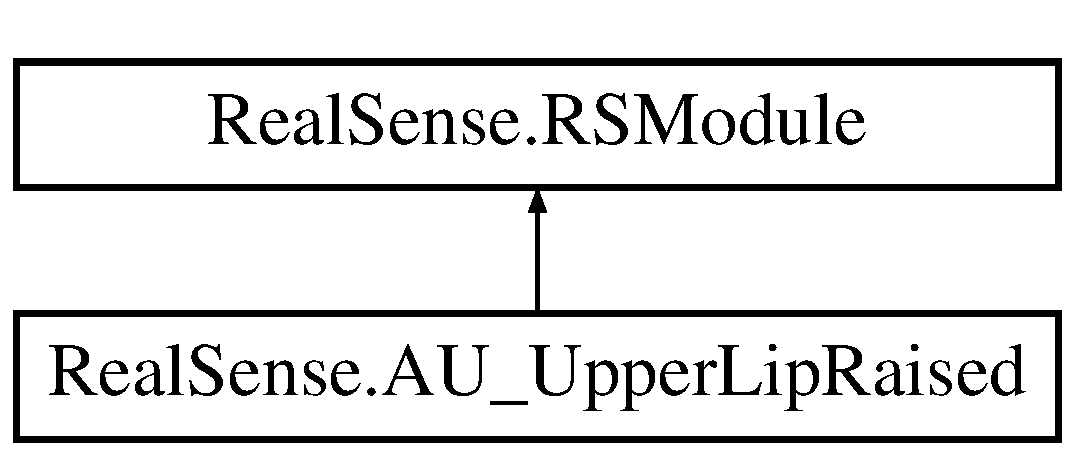
\includegraphics[height=2.000000cm]{class_real_sense_1_1_a_u___upper_lip_raised}
\end{center}
\end{figure}
\subsection*{Public Member Functions}
\begin{DoxyCompactItemize}
\item 
\textbf{ A\+U\+\_\+\+Upper\+Lip\+Raised} ()
\item 
override void \textbf{ Work} (Graphics g)
\end{DoxyCompactItemize}
\subsection*{Additional Inherited Members}


\subsection{Detailed Description}
Measures whether or not the upper lip is raised and stores its\textquotesingle{} value inside the model. \begin{DoxyAuthor}{Author}
Tobias Schramm  Hufflepuff
\end{DoxyAuthor}
Interpretation\+: 0 = Relaxed 100 = Lip up 

\subsection{Constructor \& Destructor Documentation}
\mbox{\label{class_real_sense_1_1_a_u___upper_lip_raised_a5434d7543bd2427609ca554f85173d5a}} 
\index{Real\+Sense\+::\+A\+U\+\_\+\+Upper\+Lip\+Raised@{Real\+Sense\+::\+A\+U\+\_\+\+Upper\+Lip\+Raised}!A\+U\+\_\+\+Upper\+Lip\+Raised@{A\+U\+\_\+\+Upper\+Lip\+Raised}}
\index{A\+U\+\_\+\+Upper\+Lip\+Raised@{A\+U\+\_\+\+Upper\+Lip\+Raised}!Real\+Sense\+::\+A\+U\+\_\+\+Upper\+Lip\+Raised@{Real\+Sense\+::\+A\+U\+\_\+\+Upper\+Lip\+Raised}}
\subsubsection{A\+U\+\_\+\+Upper\+Lip\+Raised()}
{\footnotesize\ttfamily Real\+Sense.\+A\+U\+\_\+\+Upper\+Lip\+Raised.\+A\+U\+\_\+\+Upper\+Lip\+Raised (\begin{DoxyParamCaption}{ }\end{DoxyParamCaption})}

Initializes the AU by setting up the default value boundaries. 

\subsection{Member Function Documentation}
\mbox{\label{class_real_sense_1_1_a_u___upper_lip_raised_a22ea7b3343701718bb2aea731850d81a}} 
\index{Real\+Sense\+::\+A\+U\+\_\+\+Upper\+Lip\+Raised@{Real\+Sense\+::\+A\+U\+\_\+\+Upper\+Lip\+Raised}!Work@{Work}}
\index{Work@{Work}!Real\+Sense\+::\+A\+U\+\_\+\+Upper\+Lip\+Raised@{Real\+Sense\+::\+A\+U\+\_\+\+Upper\+Lip\+Raised}}
\subsubsection{Work()}
{\footnotesize\ttfamily override void Real\+Sense.\+A\+U\+\_\+\+Upper\+Lip\+Raised.\+Work (\begin{DoxyParamCaption}\item[{Graphics}]{g }\end{DoxyParamCaption})\hspace{0.3cm}{\ttfamily [virtual]}}

Calculates the average difference between the upper lip and the nose to measure in which direction (and how far) it was moved over a set number of frames and prints its\textquotesingle{} debug-\/message to the \doxyref{Camera\+View}{p.}{class_real_sense_1_1_camera_view} when debug is enabled. 
\begin{DoxyParams}{Parameters}
{\em Graphics} & g for the view \\
\hline
\end{DoxyParams}


Implements \textbf{ Real\+Sense.\+R\+S\+Module} \doxyref{}{p.}{class_real_sense_1_1_r_s_module_a2ec830b7932ee7c0077d473f81c73867}.



The documentation for this class was generated from the following file\+:\begin{DoxyCompactItemize}
\item 
Action\+Units/\textbf{ A\+U\+\_\+\+Upper\+Lip\+Raised.\+cs}\end{DoxyCompactItemize}

\section{Real\+Sense.\+Camera\+View Class Reference}
\label{class_real_sense_1_1_camera_view}\index{Real\+Sense.\+Camera\+View@{Real\+Sense.\+Camera\+View}}
Inheritance diagram for Real\+Sense.\+Camera\+View\+:\begin{figure}[H]
\begin{center}
\leavevmode
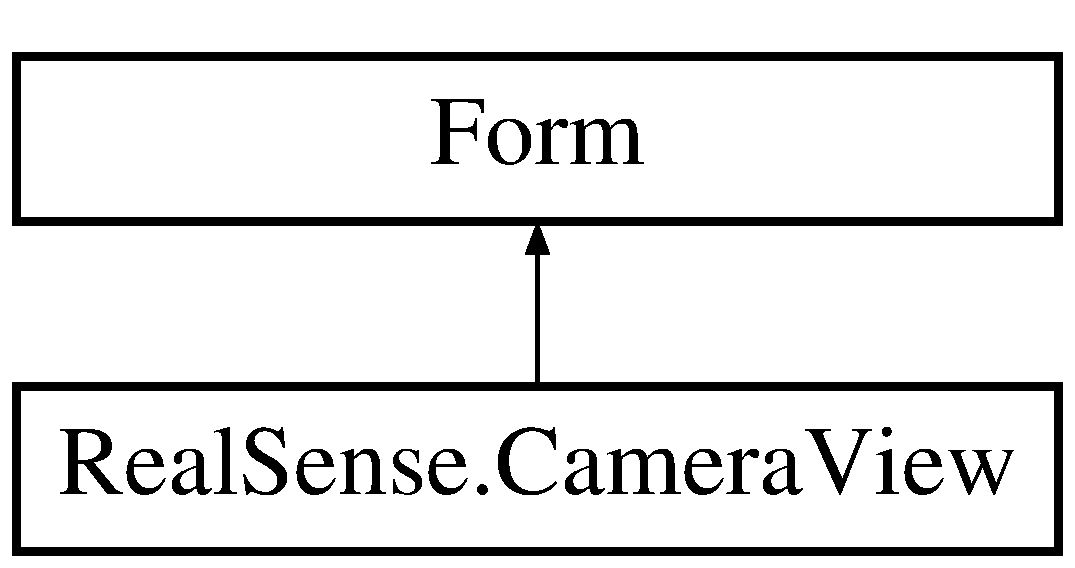
\includegraphics[height=2.000000cm]{class_real_sense_1_1_camera_view}
\end{center}
\end{figure}
\subsection*{Public Member Functions}
\begin{DoxyCompactItemize}
\item 
\textbf{ Camera\+View} (\textbf{ Model} model, \textbf{ Model.\+M\+O\+DE} m)
\item 
void \textbf{ Add\+Component} (Control c)
\end{DoxyCompactItemize}
\subsection*{Properties}
\begin{DoxyCompactItemize}
\item 
int \textbf{ Debug\+\_\+Y}\hspace{0.3cm}{\ttfamily  [get, set]}
\item 
Boolean \textbf{ Reset\+Modules}\hspace{0.3cm}{\ttfamily  [set]}
\item 
Bitmap \textbf{ Color\+Bitmap}\hspace{0.3cm}{\ttfamily  [get]}
\end{DoxyCompactItemize}


\subsection{Detailed Description}
Main-\/\+UI for testing-\/ and presentation-\/purposes \begin{DoxyAuthor}{Author}
\+: David Rosenbusch  Hufflepuff 
\end{DoxyAuthor}


\subsection{Constructor \& Destructor Documentation}
\mbox{\label{class_real_sense_1_1_camera_view_ac7f93adbed37d386412a051e6f93f978}} 
\index{Real\+Sense\+::\+Camera\+View@{Real\+Sense\+::\+Camera\+View}!Camera\+View@{Camera\+View}}
\index{Camera\+View@{Camera\+View}!Real\+Sense\+::\+Camera\+View@{Real\+Sense\+::\+Camera\+View}}
\subsubsection{Camera\+View()}
{\footnotesize\ttfamily Real\+Sense.\+Camera\+View.\+Camera\+View (\begin{DoxyParamCaption}\item[{\textbf{ Model}}]{model,  }\item[{\textbf{ Model.\+M\+O\+DE}}]{m }\end{DoxyParamCaption})}

Initialises View and starts updater Thread 
\begin{DoxyParams}{Parameters}
{\em model} & -\/ reference to data model \\
\hline
{\em Mode.\+Mode} & m -\/ mode the UI should run \\
\hline
\end{DoxyParams}


\subsection{Member Function Documentation}
\mbox{\label{class_real_sense_1_1_camera_view_a67c8ee2cdbf0caf43e48043d90c0d549}} 
\index{Real\+Sense\+::\+Camera\+View@{Real\+Sense\+::\+Camera\+View}!Add\+Component@{Add\+Component}}
\index{Add\+Component@{Add\+Component}!Real\+Sense\+::\+Camera\+View@{Real\+Sense\+::\+Camera\+View}}
\subsubsection{Add\+Component()}
{\footnotesize\ttfamily void Real\+Sense.\+Camera\+View.\+Add\+Component (\begin{DoxyParamCaption}\item[{Control}]{c }\end{DoxyParamCaption})}

Add a component to the UI (thread-\/safe)


\begin{DoxyParams}{Parameters}
{\em Control} & c, control to be added \\
\hline
\end{DoxyParams}


\subsection{Property Documentation}
\mbox{\label{class_real_sense_1_1_camera_view_a487ce7be920e8f6742d704d97a6057dc}} 
\index{Real\+Sense\+::\+Camera\+View@{Real\+Sense\+::\+Camera\+View}!Color\+Bitmap@{Color\+Bitmap}}
\index{Color\+Bitmap@{Color\+Bitmap}!Real\+Sense\+::\+Camera\+View@{Real\+Sense\+::\+Camera\+View}}
\subsubsection{Color\+Bitmap}
{\footnotesize\ttfamily Bitmap Real\+Sense.\+Camera\+View.\+Color\+Bitmap\hspace{0.3cm}{\ttfamily [get]}}

\mbox{\label{class_real_sense_1_1_camera_view_a5cc5cea08df7b36da52efba2a166e361}} 
\index{Real\+Sense\+::\+Camera\+View@{Real\+Sense\+::\+Camera\+View}!Debug\+\_\+Y@{Debug\+\_\+Y}}
\index{Debug\+\_\+Y@{Debug\+\_\+Y}!Real\+Sense\+::\+Camera\+View@{Real\+Sense\+::\+Camera\+View}}
\subsubsection{Debug\+\_\+Y}
{\footnotesize\ttfamily int Real\+Sense.\+Camera\+View.\+Debug\+\_\+Y\hspace{0.3cm}{\ttfamily [get]}, {\ttfamily [set]}}

Current y-\/coordinate of debug-\/messages \mbox{\label{class_real_sense_1_1_camera_view_a342611e6157bb18b9c097186b3b9bee0}} 
\index{Real\+Sense\+::\+Camera\+View@{Real\+Sense\+::\+Camera\+View}!Reset\+Modules@{Reset\+Modules}}
\index{Reset\+Modules@{Reset\+Modules}!Real\+Sense\+::\+Camera\+View@{Real\+Sense\+::\+Camera\+View}}
\subsubsection{Reset\+Modules}
{\footnotesize\ttfamily Boolean Real\+Sense.\+Camera\+View.\+Reset\+Modules\hspace{0.3cm}{\ttfamily [set]}}



The documentation for this class was generated from the following file\+:\begin{DoxyCompactItemize}
\item 
Framework/\textbf{ Camera\+View.\+cs}\end{DoxyCompactItemize}

\hypertarget{class_real_sense_1_1_e_m___anger}{}\section{Real\+Sense.\+E\+M\+\_\+\+Anger Class Reference}
\label{class_real_sense_1_1_e_m___anger}\index{Real\+Sense.\+E\+M\+\_\+\+Anger@{Real\+Sense.\+E\+M\+\_\+\+Anger}}
Inheritance diagram for Real\+Sense.\+E\+M\+\_\+\+Anger\+:\begin{figure}[H]
\begin{center}
\leavevmode
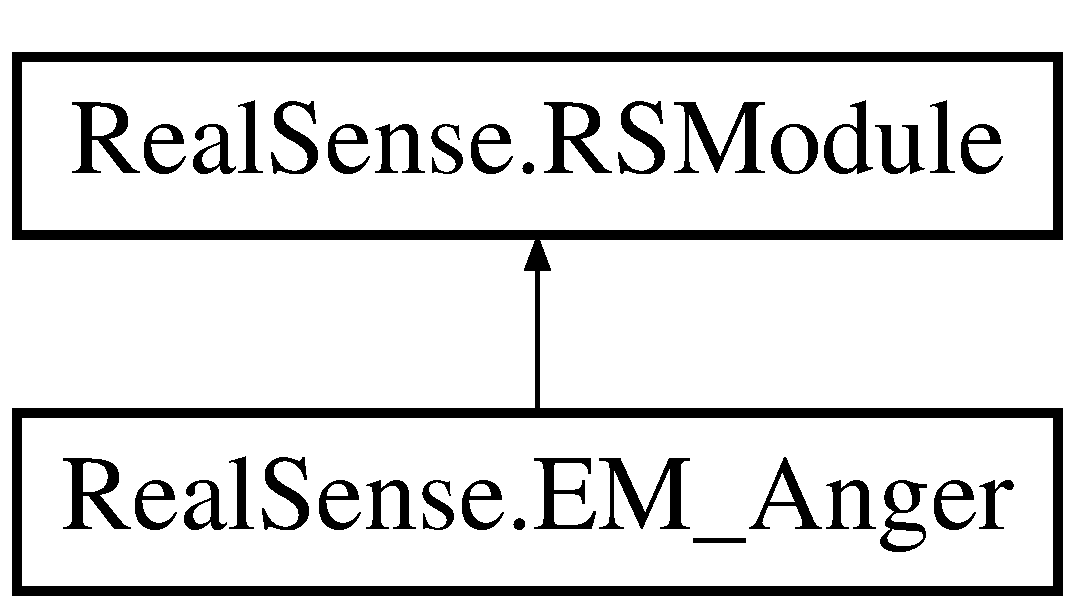
\includegraphics[height=2.000000cm]{class_real_sense_1_1_e_m___anger}
\end{center}
\end{figure}
\subsection*{Public Member Functions}
\begin{DoxyCompactItemize}
\item 
\hyperlink{class_real_sense_1_1_e_m___anger_a843c377f0f47a7e016968dbccdcbc819}{E\+M\+\_\+\+Anger} ()
\item 
override void \hyperlink{class_real_sense_1_1_e_m___anger_a5c1f3b6b7e84ee926869828a3cfe532a}{Work} (Graphics g)
\end{DoxyCompactItemize}
\subsection*{Additional Inherited Members}


\subsection{Detailed Description}
Measures the percentage value of anger. \begin{DoxyAuthor}{Author}
Tanja 
\end{DoxyAuthor}


Definition at line 14 of file E\+M\+\_\+\+Anger.\+cs.



\subsection{Constructor \& Destructor Documentation}
\mbox{\Hypertarget{class_real_sense_1_1_e_m___anger_a843c377f0f47a7e016968dbccdcbc819}\label{class_real_sense_1_1_e_m___anger_a843c377f0f47a7e016968dbccdcbc819}} 
\index{Real\+Sense\+::\+E\+M\+\_\+\+Anger@{Real\+Sense\+::\+E\+M\+\_\+\+Anger}!E\+M\+\_\+\+Anger@{E\+M\+\_\+\+Anger}}
\index{E\+M\+\_\+\+Anger@{E\+M\+\_\+\+Anger}!Real\+Sense\+::\+E\+M\+\_\+\+Anger@{Real\+Sense\+::\+E\+M\+\_\+\+Anger}}
\subsubsection{\texorpdfstring{E\+M\+\_\+\+Anger()}{EM\_Anger()}}
{\footnotesize\ttfamily Real\+Sense.\+E\+M\+\_\+\+Anger.\+E\+M\+\_\+\+Anger (\begin{DoxyParamCaption}{ }\end{DoxyParamCaption})}

Initializes the EM, setting the debug-\/flag to true by default 

Definition at line 21 of file E\+M\+\_\+\+Anger.\+cs.



\subsection{Member Function Documentation}
\mbox{\Hypertarget{class_real_sense_1_1_e_m___anger_a5c1f3b6b7e84ee926869828a3cfe532a}\label{class_real_sense_1_1_e_m___anger_a5c1f3b6b7e84ee926869828a3cfe532a}} 
\index{Real\+Sense\+::\+E\+M\+\_\+\+Anger@{Real\+Sense\+::\+E\+M\+\_\+\+Anger}!Work@{Work}}
\index{Work@{Work}!Real\+Sense\+::\+E\+M\+\_\+\+Anger@{Real\+Sense\+::\+E\+M\+\_\+\+Anger}}
\subsubsection{\texorpdfstring{Work()}{Work()}}
{\footnotesize\ttfamily override void Real\+Sense.\+E\+M\+\_\+\+Anger.\+Work (\begin{DoxyParamCaption}\item[{Graphics}]{g }\end{DoxyParamCaption})\hspace{0.3cm}{\ttfamily [virtual]}}

Computes the percentage Value of Anger in the current Frame. 
\begin{DoxyParams}{Parameters}
{\em Graphics} & g for the view \\
\hline
\end{DoxyParams}


Implements \hyperlink{class_real_sense_1_1_r_s_module_a2ec830b7932ee7c0077d473f81c73867}{Real\+Sense.\+R\+S\+Module}.



Definition at line 31 of file E\+M\+\_\+\+Anger.\+cs.



The documentation for this class was generated from the following file\+:\begin{DoxyCompactItemize}
\item 
C\+:/\+Users/nutzer/\+Documents/\+Git\+Hub/\+Real\+Sense/\+Emotions/\hyperlink{_e_m___anger_8cs}{E\+M\+\_\+\+Anger.\+cs}\end{DoxyCompactItemize}

\section{Real\+Sense.\+Emotions.\+E\+M\+\_\+\+Contempt Class Reference}
\label{class_real_sense_1_1_emotions_1_1_e_m___contempt}\index{Real\+Sense.\+Emotions.\+E\+M\+\_\+\+Contempt@{Real\+Sense.\+Emotions.\+E\+M\+\_\+\+Contempt}}
Inheritance diagram for Real\+Sense.\+Emotions.\+E\+M\+\_\+\+Contempt\+:\begin{figure}[H]
\begin{center}
\leavevmode
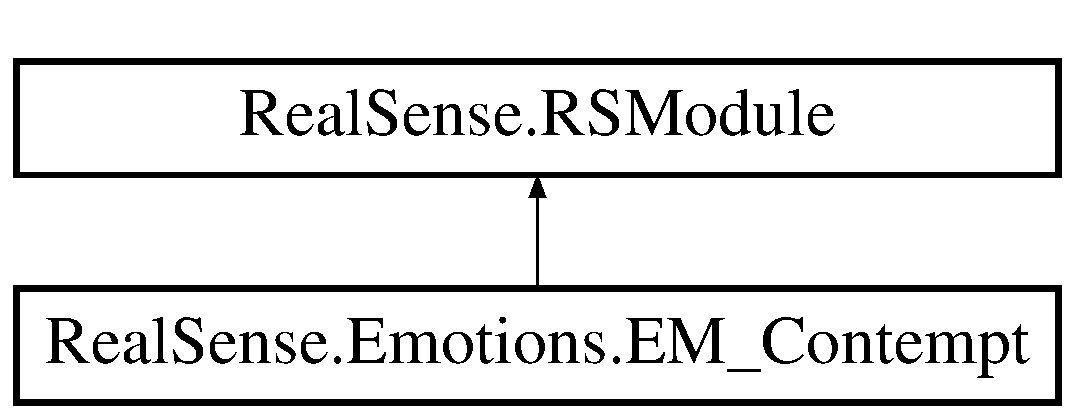
\includegraphics[height=2.000000cm]{class_real_sense_1_1_emotions_1_1_e_m___contempt}
\end{center}
\end{figure}
\subsection*{Public Member Functions}
\begin{DoxyCompactItemize}
\item 
\textbf{ E\+M\+\_\+\+Contempt} ()
\item 
override void \textbf{ Work} (Graphics g)
\end{DoxyCompactItemize}
\subsection*{Additional Inherited Members}


\subsection{Detailed Description}
Measures the percentage value of contempt. \begin{DoxyAuthor}{Author}
Tanja 
\end{DoxyAuthor}


\subsection{Constructor \& Destructor Documentation}
\mbox{\label{class_real_sense_1_1_emotions_1_1_e_m___contempt_af2203e6c540c756cd6b8d0190d04c46f}} 
\index{Real\+Sense\+::\+Emotions\+::\+E\+M\+\_\+\+Contempt@{Real\+Sense\+::\+Emotions\+::\+E\+M\+\_\+\+Contempt}!E\+M\+\_\+\+Contempt@{E\+M\+\_\+\+Contempt}}
\index{E\+M\+\_\+\+Contempt@{E\+M\+\_\+\+Contempt}!Real\+Sense\+::\+Emotions\+::\+E\+M\+\_\+\+Contempt@{Real\+Sense\+::\+Emotions\+::\+E\+M\+\_\+\+Contempt}}
\subsubsection{E\+M\+\_\+\+Contempt()}
{\footnotesize\ttfamily Real\+Sense.\+Emotions.\+E\+M\+\_\+\+Contempt.\+E\+M\+\_\+\+Contempt (\begin{DoxyParamCaption}{ }\end{DoxyParamCaption})}

Initializes the EM, setting the debug-\/flag to true by default Also sets up a default boundary of max-\/, min, extreme-\/ and tolerance-\/values 

\subsection{Member Function Documentation}
\mbox{\label{class_real_sense_1_1_emotions_1_1_e_m___contempt_a7ea208f926c1888f028cbe6d6fe14e2f}} 
\index{Real\+Sense\+::\+Emotions\+::\+E\+M\+\_\+\+Contempt@{Real\+Sense\+::\+Emotions\+::\+E\+M\+\_\+\+Contempt}!Work@{Work}}
\index{Work@{Work}!Real\+Sense\+::\+Emotions\+::\+E\+M\+\_\+\+Contempt@{Real\+Sense\+::\+Emotions\+::\+E\+M\+\_\+\+Contempt}}
\subsubsection{Work()}
{\footnotesize\ttfamily override void Real\+Sense.\+Emotions.\+E\+M\+\_\+\+Contempt.\+Work (\begin{DoxyParamCaption}\item[{Graphics}]{g }\end{DoxyParamCaption})\hspace{0.3cm}{\ttfamily [virtual]}}

Computes the percentage Value of contempt in the current Frame. 
\begin{DoxyParams}{Parameters}
{\em Graphics} & g for the view \\
\hline
\end{DoxyParams}


Implements \textbf{ Real\+Sense.\+R\+S\+Module} \doxyref{}{p.}{class_real_sense_1_1_r_s_module_a2ec830b7932ee7c0077d473f81c73867}.



The documentation for this class was generated from the following file\+:\begin{DoxyCompactItemize}
\item 
Emotions/\textbf{ E\+M\+\_\+\+Contempt.\+cs}\end{DoxyCompactItemize}

\section{Real\+Sense.\+Emotions.\+E\+M\+\_\+\+Disgust Class Reference}
\label{class_real_sense_1_1_emotions_1_1_e_m___disgust}\index{Real\+Sense.\+Emotions.\+E\+M\+\_\+\+Disgust@{Real\+Sense.\+Emotions.\+E\+M\+\_\+\+Disgust}}
Inheritance diagram for Real\+Sense.\+Emotions.\+E\+M\+\_\+\+Disgust\+:\begin{figure}[H]
\begin{center}
\leavevmode
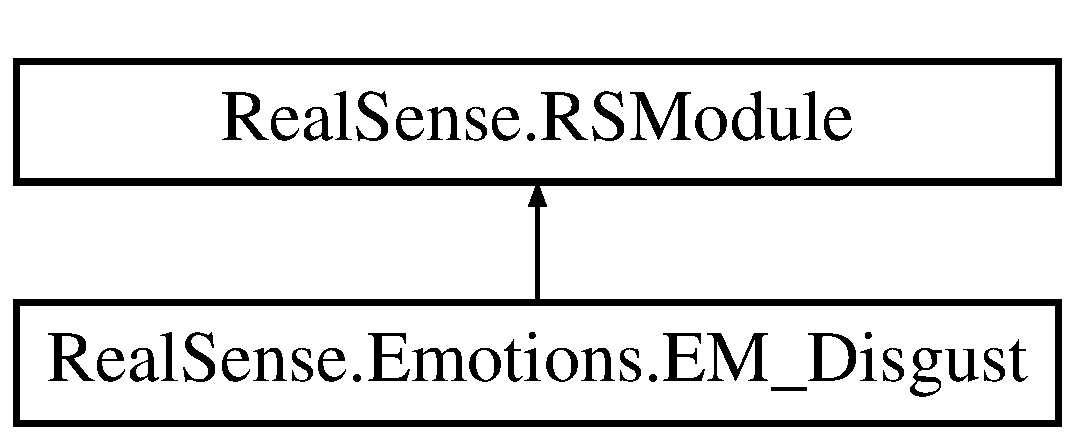
\includegraphics[height=2.000000cm]{class_real_sense_1_1_emotions_1_1_e_m___disgust}
\end{center}
\end{figure}
\subsection*{Public Member Functions}
\begin{DoxyCompactItemize}
\item 
\textbf{ E\+M\+\_\+\+Disgust} ()
\item 
override void \textbf{ Work} (Graphics g)
\end{DoxyCompactItemize}
\subsection*{Additional Inherited Members}


\subsection{Detailed Description}
Measures the percentage value of disgust. \begin{DoxyAuthor}{Author}
Tanja 
\end{DoxyAuthor}


\subsection{Constructor \& Destructor Documentation}
\mbox{\label{class_real_sense_1_1_emotions_1_1_e_m___disgust_aba892f265a554ffe99c81482b48fbed0}} 
\index{Real\+Sense\+::\+Emotions\+::\+E\+M\+\_\+\+Disgust@{Real\+Sense\+::\+Emotions\+::\+E\+M\+\_\+\+Disgust}!E\+M\+\_\+\+Disgust@{E\+M\+\_\+\+Disgust}}
\index{E\+M\+\_\+\+Disgust@{E\+M\+\_\+\+Disgust}!Real\+Sense\+::\+Emotions\+::\+E\+M\+\_\+\+Disgust@{Real\+Sense\+::\+Emotions\+::\+E\+M\+\_\+\+Disgust}}
\subsubsection{E\+M\+\_\+\+Disgust()}
{\footnotesize\ttfamily Real\+Sense.\+Emotions.\+E\+M\+\_\+\+Disgust.\+E\+M\+\_\+\+Disgust (\begin{DoxyParamCaption}{ }\end{DoxyParamCaption})}

Initializes the EM, setting the debug-\/flag to true by default Also sets up a default boundary of max-\/, min, extreme-\/ and tolerance-\/values 

\subsection{Member Function Documentation}
\mbox{\label{class_real_sense_1_1_emotions_1_1_e_m___disgust_a22cbe3025c32821d53edcb325140ccb1}} 
\index{Real\+Sense\+::\+Emotions\+::\+E\+M\+\_\+\+Disgust@{Real\+Sense\+::\+Emotions\+::\+E\+M\+\_\+\+Disgust}!Work@{Work}}
\index{Work@{Work}!Real\+Sense\+::\+Emotions\+::\+E\+M\+\_\+\+Disgust@{Real\+Sense\+::\+Emotions\+::\+E\+M\+\_\+\+Disgust}}
\subsubsection{Work()}
{\footnotesize\ttfamily override void Real\+Sense.\+Emotions.\+E\+M\+\_\+\+Disgust.\+Work (\begin{DoxyParamCaption}\item[{Graphics}]{g }\end{DoxyParamCaption})\hspace{0.3cm}{\ttfamily [virtual]}}

Computes the percentage Value of disgust in the current Frame. 
\begin{DoxyParams}{Parameters}
{\em Graphics} & g for the view \\
\hline
\end{DoxyParams}


Implements \textbf{ Real\+Sense.\+R\+S\+Module} \doxyref{}{p.}{class_real_sense_1_1_r_s_module_a2ec830b7932ee7c0077d473f81c73867}.



The documentation for this class was generated from the following file\+:\begin{DoxyCompactItemize}
\item 
Emotions/\textbf{ E\+M\+\_\+\+Disgust.\+cs}\end{DoxyCompactItemize}

\section{Real\+Sense.\+Emotions.\+E\+M\+\_\+\+Fear Class Reference}
\label{class_real_sense_1_1_emotions_1_1_e_m___fear}\index{Real\+Sense.\+Emotions.\+E\+M\+\_\+\+Fear@{Real\+Sense.\+Emotions.\+E\+M\+\_\+\+Fear}}
Inheritance diagram for Real\+Sense.\+Emotions.\+E\+M\+\_\+\+Fear\+:\begin{figure}[H]
\begin{center}
\leavevmode
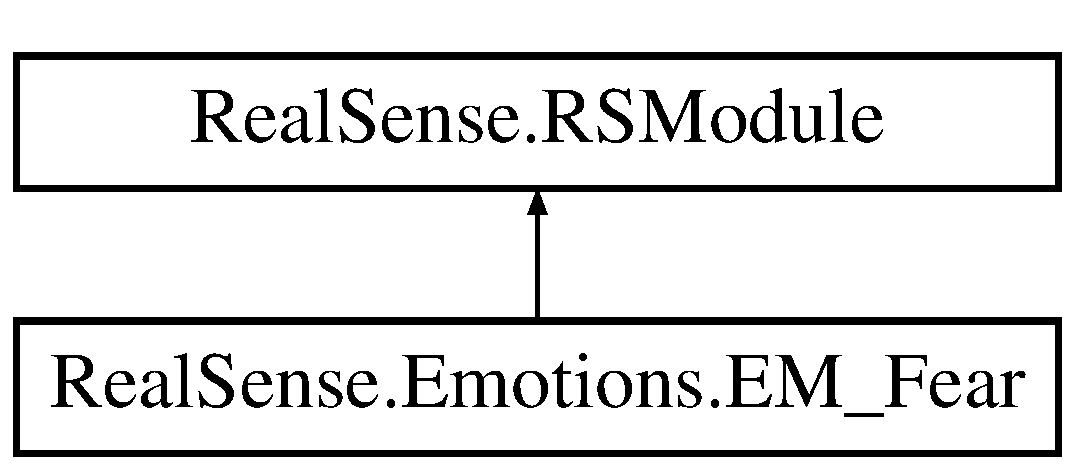
\includegraphics[height=2.000000cm]{class_real_sense_1_1_emotions_1_1_e_m___fear}
\end{center}
\end{figure}
\subsection*{Public Member Functions}
\begin{DoxyCompactItemize}
\item 
override void \textbf{ Work} (Graphics g)
\end{DoxyCompactItemize}
\subsection*{Additional Inherited Members}


\subsection{Member Function Documentation}
\mbox{\label{class_real_sense_1_1_emotions_1_1_e_m___fear_a5b417a4a8403f101585dc8c239288c54}} 
\index{Real\+Sense\+::\+Emotions\+::\+E\+M\+\_\+\+Fear@{Real\+Sense\+::\+Emotions\+::\+E\+M\+\_\+\+Fear}!Work@{Work}}
\index{Work@{Work}!Real\+Sense\+::\+Emotions\+::\+E\+M\+\_\+\+Fear@{Real\+Sense\+::\+Emotions\+::\+E\+M\+\_\+\+Fear}}
\subsubsection{Work()}
{\footnotesize\ttfamily override void Real\+Sense.\+Emotions.\+E\+M\+\_\+\+Fear.\+Work (\begin{DoxyParamCaption}\item[{Graphics}]{g }\end{DoxyParamCaption})\hspace{0.3cm}{\ttfamily [virtual]}}

Update every frame (do calculations, manipulate output Image) 
\begin{DoxyParams}{Parameters}
{\em Graphics} & g \\
\hline
\end{DoxyParams}


Implements \textbf{ Real\+Sense.\+R\+S\+Module} \doxyref{}{p.}{class_real_sense_1_1_r_s_module_a2ec830b7932ee7c0077d473f81c73867}.



The documentation for this class was generated from the following file\+:\begin{DoxyCompactItemize}
\item 
Emotions/E\+M\+\_\+\+Fear.\+cs\end{DoxyCompactItemize}

\hypertarget{class_real_sense_1_1_emotions_1_1_e_m___joy}{}\section{Real\+Sense.\+Emotions.\+E\+M\+\_\+\+Joy Class Reference}
\label{class_real_sense_1_1_emotions_1_1_e_m___joy}\index{Real\+Sense.\+Emotions.\+E\+M\+\_\+\+Joy@{Real\+Sense.\+Emotions.\+E\+M\+\_\+\+Joy}}
Inheritance diagram for Real\+Sense.\+Emotions.\+E\+M\+\_\+\+Joy\+:\begin{figure}[H]
\begin{center}
\leavevmode
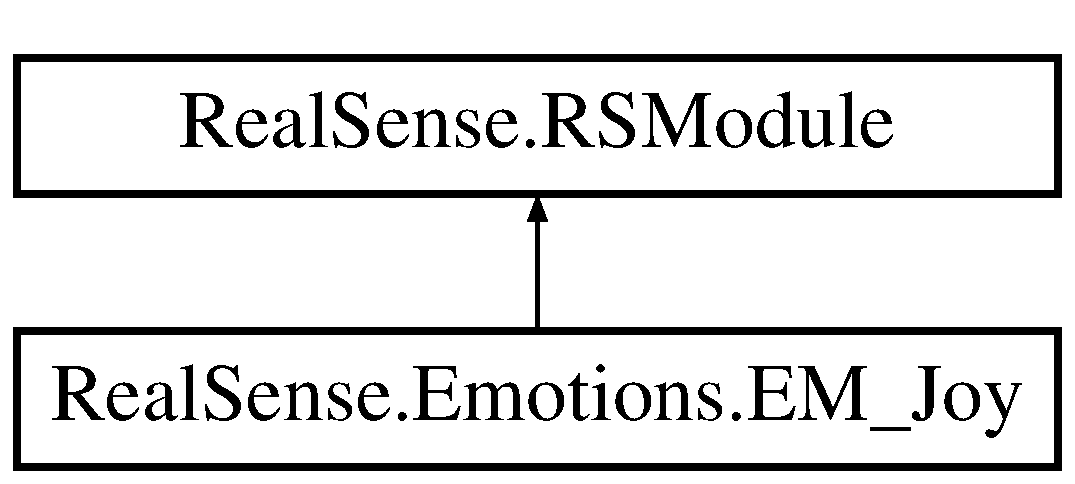
\includegraphics[height=2.000000cm]{class_real_sense_1_1_emotions_1_1_e_m___joy}
\end{center}
\end{figure}
\subsection*{Public Member Functions}
\begin{DoxyCompactItemize}
\item 
\hyperlink{class_real_sense_1_1_emotions_1_1_e_m___joy_a1e37185e1aadd7a6e9c38414b5eb22fe}{E\+M\+\_\+\+Joy} ()
\item 
override void \hyperlink{class_real_sense_1_1_emotions_1_1_e_m___joy_acce5a4daa0acfd1a10d0aac92ef278c8}{Work} (Graphics g)
\end{DoxyCompactItemize}
\subsection*{Additional Inherited Members}


\subsection{Detailed Description}


Definition at line 13 of file E\+M\+\_\+\+Joy.\+cs.



\subsection{Constructor \& Destructor Documentation}
\mbox{\Hypertarget{class_real_sense_1_1_emotions_1_1_e_m___joy_a1e37185e1aadd7a6e9c38414b5eb22fe}\label{class_real_sense_1_1_emotions_1_1_e_m___joy_a1e37185e1aadd7a6e9c38414b5eb22fe}} 
\index{Real\+Sense\+::\+Emotions\+::\+E\+M\+\_\+\+Joy@{Real\+Sense\+::\+Emotions\+::\+E\+M\+\_\+\+Joy}!E\+M\+\_\+\+Joy@{E\+M\+\_\+\+Joy}}
\index{E\+M\+\_\+\+Joy@{E\+M\+\_\+\+Joy}!Real\+Sense\+::\+Emotions\+::\+E\+M\+\_\+\+Joy@{Real\+Sense\+::\+Emotions\+::\+E\+M\+\_\+\+Joy}}
\subsubsection{\texorpdfstring{E\+M\+\_\+\+Joy()}{EM\_Joy()}}
{\footnotesize\ttfamily Real\+Sense.\+Emotions.\+E\+M\+\_\+\+Joy.\+E\+M\+\_\+\+Joy (\begin{DoxyParamCaption}{ }\end{DoxyParamCaption})}



Definition at line 20 of file E\+M\+\_\+\+Joy.\+cs.



\subsection{Member Function Documentation}
\mbox{\Hypertarget{class_real_sense_1_1_emotions_1_1_e_m___joy_acce5a4daa0acfd1a10d0aac92ef278c8}\label{class_real_sense_1_1_emotions_1_1_e_m___joy_acce5a4daa0acfd1a10d0aac92ef278c8}} 
\index{Real\+Sense\+::\+Emotions\+::\+E\+M\+\_\+\+Joy@{Real\+Sense\+::\+Emotions\+::\+E\+M\+\_\+\+Joy}!Work@{Work}}
\index{Work@{Work}!Real\+Sense\+::\+Emotions\+::\+E\+M\+\_\+\+Joy@{Real\+Sense\+::\+Emotions\+::\+E\+M\+\_\+\+Joy}}
\subsubsection{\texorpdfstring{Work()}{Work()}}
{\footnotesize\ttfamily override void Real\+Sense.\+Emotions.\+E\+M\+\_\+\+Joy.\+Work (\begin{DoxyParamCaption}\item[{Graphics}]{g }\end{DoxyParamCaption})\hspace{0.3cm}{\ttfamily [virtual]}}

Computes the percentage Value of Joy in the current Frame. 
\begin{DoxyParams}{Parameters}
{\em Graphics} & g for the view \\
\hline
\end{DoxyParams}


Implements \hyperlink{class_real_sense_1_1_r_s_module_a2ec830b7932ee7c0077d473f81c73867}{Real\+Sense.\+R\+S\+Module}.



Definition at line 29 of file E\+M\+\_\+\+Joy.\+cs.



The documentation for this class was generated from the following file\+:\begin{DoxyCompactItemize}
\item 
Emotions/\hyperlink{_e_m___joy_8cs}{E\+M\+\_\+\+Joy.\+cs}\end{DoxyCompactItemize}

\hypertarget{class_real_sense_1_1_emotions_1_1_e_m___sadness}{}\section{Real\+Sense.\+Emotions.\+E\+M\+\_\+\+Sadness Class Reference}
\label{class_real_sense_1_1_emotions_1_1_e_m___sadness}\index{Real\+Sense.\+Emotions.\+E\+M\+\_\+\+Sadness@{Real\+Sense.\+Emotions.\+E\+M\+\_\+\+Sadness}}
Inheritance diagram for Real\+Sense.\+Emotions.\+E\+M\+\_\+\+Sadness\+:\begin{figure}[H]
\begin{center}
\leavevmode
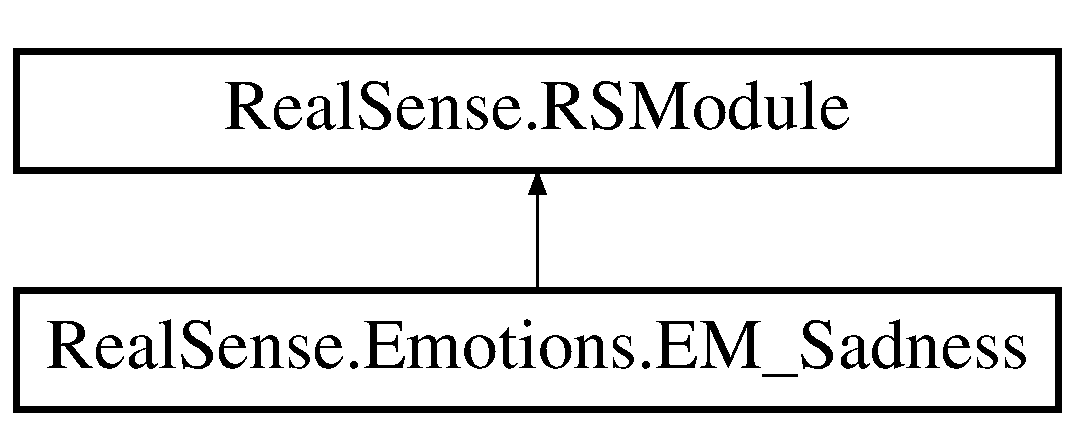
\includegraphics[height=2.000000cm]{class_real_sense_1_1_emotions_1_1_e_m___sadness}
\end{center}
\end{figure}
\subsection*{Public Member Functions}
\begin{DoxyCompactItemize}
\item 
\hyperlink{class_real_sense_1_1_emotions_1_1_e_m___sadness_ad0a149a2f1b6aefd5fedd870a1cefb00}{E\+M\+\_\+\+Sadness} ()
\item 
override void \hyperlink{class_real_sense_1_1_emotions_1_1_e_m___sadness_a45cf23f5c3382bc9769abf1ef401ade1}{Work} (Graphics g)
\end{DoxyCompactItemize}
\subsection*{Additional Inherited Members}


\subsection{Detailed Description}
Measures the percentage value of sadness. \begin{DoxyAuthor}{Author}
Tanja 
\end{DoxyAuthor}


Definition at line 14 of file E\+M\+\_\+\+Sadness.\+cs.



\subsection{Constructor \& Destructor Documentation}
\mbox{\Hypertarget{class_real_sense_1_1_emotions_1_1_e_m___sadness_ad0a149a2f1b6aefd5fedd870a1cefb00}\label{class_real_sense_1_1_emotions_1_1_e_m___sadness_ad0a149a2f1b6aefd5fedd870a1cefb00}} 
\index{Real\+Sense\+::\+Emotions\+::\+E\+M\+\_\+\+Sadness@{Real\+Sense\+::\+Emotions\+::\+E\+M\+\_\+\+Sadness}!E\+M\+\_\+\+Sadness@{E\+M\+\_\+\+Sadness}}
\index{E\+M\+\_\+\+Sadness@{E\+M\+\_\+\+Sadness}!Real\+Sense\+::\+Emotions\+::\+E\+M\+\_\+\+Sadness@{Real\+Sense\+::\+Emotions\+::\+E\+M\+\_\+\+Sadness}}
\subsubsection{\texorpdfstring{E\+M\+\_\+\+Sadness()}{EM\_Sadness()}}
{\footnotesize\ttfamily Real\+Sense.\+Emotions.\+E\+M\+\_\+\+Sadness.\+E\+M\+\_\+\+Sadness (\begin{DoxyParamCaption}{ }\end{DoxyParamCaption})}

Initializes the EM, setting the debug-\/flag to true by default 

Definition at line 19 of file E\+M\+\_\+\+Sadness.\+cs.



\subsection{Member Function Documentation}
\mbox{\Hypertarget{class_real_sense_1_1_emotions_1_1_e_m___sadness_a45cf23f5c3382bc9769abf1ef401ade1}\label{class_real_sense_1_1_emotions_1_1_e_m___sadness_a45cf23f5c3382bc9769abf1ef401ade1}} 
\index{Real\+Sense\+::\+Emotions\+::\+E\+M\+\_\+\+Sadness@{Real\+Sense\+::\+Emotions\+::\+E\+M\+\_\+\+Sadness}!Work@{Work}}
\index{Work@{Work}!Real\+Sense\+::\+Emotions\+::\+E\+M\+\_\+\+Sadness@{Real\+Sense\+::\+Emotions\+::\+E\+M\+\_\+\+Sadness}}
\subsubsection{\texorpdfstring{Work()}{Work()}}
{\footnotesize\ttfamily override void Real\+Sense.\+Emotions.\+E\+M\+\_\+\+Sadness.\+Work (\begin{DoxyParamCaption}\item[{Graphics}]{g }\end{DoxyParamCaption})\hspace{0.3cm}{\ttfamily [virtual]}}

Computes the percentage Value of Sadness in the current Frame. 
\begin{DoxyParams}{Parameters}
{\em Graphics} & g for the view \\
\hline
\end{DoxyParams}


Implements \hyperlink{class_real_sense_1_1_r_s_module_a2ec830b7932ee7c0077d473f81c73867}{Real\+Sense.\+R\+S\+Module}.



Definition at line 29 of file E\+M\+\_\+\+Sadness.\+cs.



The documentation for this class was generated from the following file\+:\begin{DoxyCompactItemize}
\item 
C\+:/\+Users/nutzer/\+Documents/\+Git\+Hub/\+Real\+Sense/\+Emotions/\hyperlink{_e_m___sadness_8cs}{E\+M\+\_\+\+Sadness.\+cs}\end{DoxyCompactItemize}

\hypertarget{class_real_sense_1_1_emotions_1_1_e_m___surprise}{}\section{Real\+Sense.\+Emotions.\+E\+M\+\_\+\+Surprise Class Reference}
\label{class_real_sense_1_1_emotions_1_1_e_m___surprise}\index{Real\+Sense.\+Emotions.\+E\+M\+\_\+\+Surprise@{Real\+Sense.\+Emotions.\+E\+M\+\_\+\+Surprise}}
Inheritance diagram for Real\+Sense.\+Emotions.\+E\+M\+\_\+\+Surprise\+:\begin{figure}[H]
\begin{center}
\leavevmode
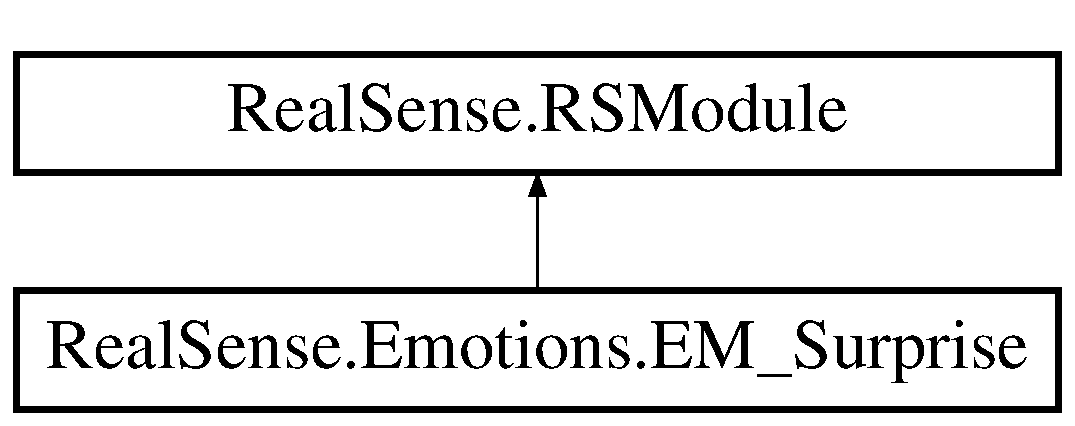
\includegraphics[height=2.000000cm]{class_real_sense_1_1_emotions_1_1_e_m___surprise}
\end{center}
\end{figure}
\subsection*{Public Member Functions}
\begin{DoxyCompactItemize}
\item 
\hyperlink{class_real_sense_1_1_emotions_1_1_e_m___surprise_a95c89a129f31134f35b0d34a212e7d29}{E\+M\+\_\+\+Surprise} ()
\item 
override void \hyperlink{class_real_sense_1_1_emotions_1_1_e_m___surprise_a08040934bb081596a4b02b483dc3a662}{Work} (Graphics g)
\end{DoxyCompactItemize}
\subsection*{Additional Inherited Members}


\subsection{Detailed Description}


Definition at line 13 of file E\+M\+\_\+\+Surprise.\+cs.



\subsection{Constructor \& Destructor Documentation}
\mbox{\Hypertarget{class_real_sense_1_1_emotions_1_1_e_m___surprise_a95c89a129f31134f35b0d34a212e7d29}\label{class_real_sense_1_1_emotions_1_1_e_m___surprise_a95c89a129f31134f35b0d34a212e7d29}} 
\index{Real\+Sense\+::\+Emotions\+::\+E\+M\+\_\+\+Surprise@{Real\+Sense\+::\+Emotions\+::\+E\+M\+\_\+\+Surprise}!E\+M\+\_\+\+Surprise@{E\+M\+\_\+\+Surprise}}
\index{E\+M\+\_\+\+Surprise@{E\+M\+\_\+\+Surprise}!Real\+Sense\+::\+Emotions\+::\+E\+M\+\_\+\+Surprise@{Real\+Sense\+::\+Emotions\+::\+E\+M\+\_\+\+Surprise}}
\subsubsection{\texorpdfstring{E\+M\+\_\+\+Surprise()}{EM\_Surprise()}}
{\footnotesize\ttfamily Real\+Sense.\+Emotions.\+E\+M\+\_\+\+Surprise.\+E\+M\+\_\+\+Surprise (\begin{DoxyParamCaption}{ }\end{DoxyParamCaption})}



Definition at line 19 of file E\+M\+\_\+\+Surprise.\+cs.



\subsection{Member Function Documentation}
\mbox{\Hypertarget{class_real_sense_1_1_emotions_1_1_e_m___surprise_a08040934bb081596a4b02b483dc3a662}\label{class_real_sense_1_1_emotions_1_1_e_m___surprise_a08040934bb081596a4b02b483dc3a662}} 
\index{Real\+Sense\+::\+Emotions\+::\+E\+M\+\_\+\+Surprise@{Real\+Sense\+::\+Emotions\+::\+E\+M\+\_\+\+Surprise}!Work@{Work}}
\index{Work@{Work}!Real\+Sense\+::\+Emotions\+::\+E\+M\+\_\+\+Surprise@{Real\+Sense\+::\+Emotions\+::\+E\+M\+\_\+\+Surprise}}
\subsubsection{\texorpdfstring{Work()}{Work()}}
{\footnotesize\ttfamily override void Real\+Sense.\+Emotions.\+E\+M\+\_\+\+Surprise.\+Work (\begin{DoxyParamCaption}\item[{Graphics}]{g }\end{DoxyParamCaption})\hspace{0.3cm}{\ttfamily [virtual]}}

Computes the percentage Value of Surprise in the current Frame. 
\begin{DoxyParams}{Parameters}
{\em Graphics} & g for the view \\
\hline
\end{DoxyParams}


Implements \hyperlink{class_real_sense_1_1_r_s_module_a2ec830b7932ee7c0077d473f81c73867}{Real\+Sense.\+R\+S\+Module}.



Definition at line 28 of file E\+M\+\_\+\+Surprise.\+cs.



The documentation for this class was generated from the following file\+:\begin{DoxyCompactItemize}
\item 
Emotions/\hyperlink{_e_m___surprise_8cs}{E\+M\+\_\+\+Surprise.\+cs}\end{DoxyCompactItemize}

\hypertarget{class_real_sense_1_1_face_recorder}{}\section{Real\+Sense.\+Face\+Recorder Class Reference}
\label{class_real_sense_1_1_face_recorder}\index{Real\+Sense.\+Face\+Recorder@{Real\+Sense.\+Face\+Recorder}}
Inheritance diagram for Real\+Sense.\+Face\+Recorder\+:\begin{figure}[H]
\begin{center}
\leavevmode
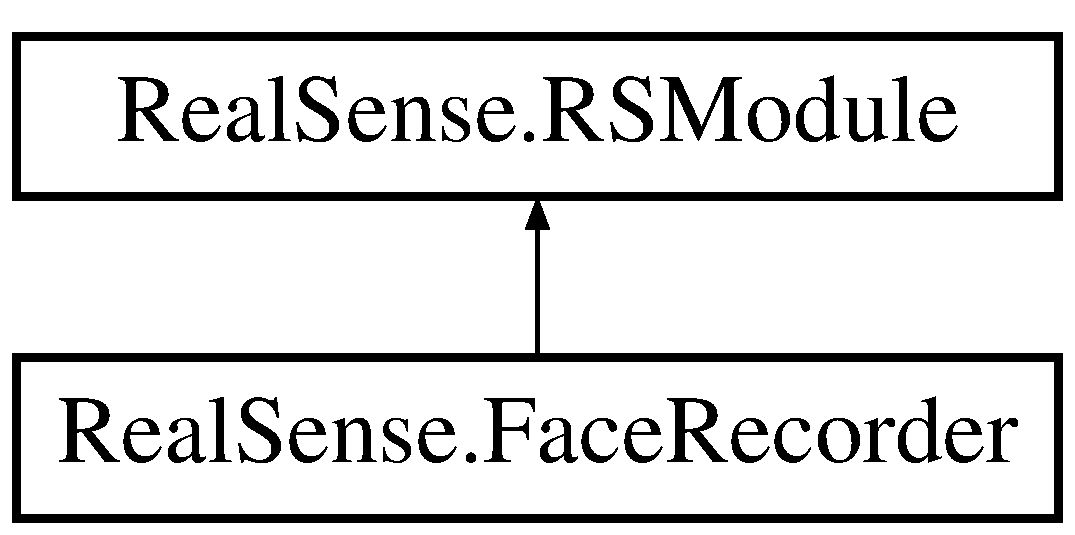
\includegraphics[height=2.000000cm]{class_real_sense_1_1_face_recorder}
\end{center}
\end{figure}
\subsection*{Public Member Functions}
\begin{DoxyCompactItemize}
\item 
\hyperlink{class_real_sense_1_1_face_recorder_a782589b2a536a93d548f1efab49c6bcd}{Face\+Recorder} ()
\item 
override void \hyperlink{class_real_sense_1_1_face_recorder_a315985241eb6c21f6393d8104a967eb6}{Key\+Trigger} (int key)
\item 
override void \hyperlink{class_real_sense_1_1_face_recorder_a2adae8c9db76fe9617e99795b4fa5e0e}{Work} (Graphics g)
\end{DoxyCompactItemize}
\subsection*{Properties}
\begin{DoxyCompactItemize}
\item 
bool \hyperlink{class_real_sense_1_1_face_recorder_a3dd841901321c20b2bba9067fc67bddd}{Recording}\hspace{0.3cm}{\ttfamily  \mbox{[}get\mbox{]}}
\item 
int \hyperlink{class_real_sense_1_1_face_recorder_a4f1a094d0321d299feb5aa0e3553b506}{Recording\+Index}\hspace{0.3cm}{\ttfamily  \mbox{[}get, set\mbox{]}}
\end{DoxyCompactItemize}
\subsection*{Additional Inherited Members}


\subsection{Detailed Description}


Definition at line 17 of file Face\+Recorder.\+cs.



\subsection{Constructor \& Destructor Documentation}
\mbox{\Hypertarget{class_real_sense_1_1_face_recorder_a782589b2a536a93d548f1efab49c6bcd}\label{class_real_sense_1_1_face_recorder_a782589b2a536a93d548f1efab49c6bcd}} 
\index{Real\+Sense\+::\+Face\+Recorder@{Real\+Sense\+::\+Face\+Recorder}!Face\+Recorder@{Face\+Recorder}}
\index{Face\+Recorder@{Face\+Recorder}!Real\+Sense\+::\+Face\+Recorder@{Real\+Sense\+::\+Face\+Recorder}}
\subsubsection{\texorpdfstring{Face\+Recorder()}{FaceRecorder()}}
{\footnotesize\ttfamily Real\+Sense.\+Face\+Recorder.\+Face\+Recorder (\begin{DoxyParamCaption}{ }\end{DoxyParamCaption})}

Initializes the key\+Triggers and an empty buffer for the landmark-\/data. 

Definition at line 30 of file Face\+Recorder.\+cs.



\subsection{Member Function Documentation}
\mbox{\Hypertarget{class_real_sense_1_1_face_recorder_a315985241eb6c21f6393d8104a967eb6}\label{class_real_sense_1_1_face_recorder_a315985241eb6c21f6393d8104a967eb6}} 
\index{Real\+Sense\+::\+Face\+Recorder@{Real\+Sense\+::\+Face\+Recorder}!Key\+Trigger@{Key\+Trigger}}
\index{Key\+Trigger@{Key\+Trigger}!Real\+Sense\+::\+Face\+Recorder@{Real\+Sense\+::\+Face\+Recorder}}
\subsubsection{\texorpdfstring{Key\+Trigger()}{KeyTrigger()}}
{\footnotesize\ttfamily override void Real\+Sense.\+Face\+Recorder.\+Key\+Trigger (\begin{DoxyParamCaption}\item[{int}]{key }\end{DoxyParamCaption})\hspace{0.3cm}{\ttfamily [virtual]}}

The current recording\textquotesingle{}s type is determined by the key that is pressed to trigger the recording. 
\begin{DoxyParams}{Parameters}
{\em key} & -\/ key that triggers the module \\
\hline
\end{DoxyParams}


Reimplemented from \hyperlink{class_real_sense_1_1_r_s_module_a8434d4aa8c289766b24e67cabb7e9471}{Real\+Sense.\+R\+S\+Module}.



Definition at line 42 of file Face\+Recorder.\+cs.

\mbox{\Hypertarget{class_real_sense_1_1_face_recorder_a2adae8c9db76fe9617e99795b4fa5e0e}\label{class_real_sense_1_1_face_recorder_a2adae8c9db76fe9617e99795b4fa5e0e}} 
\index{Real\+Sense\+::\+Face\+Recorder@{Real\+Sense\+::\+Face\+Recorder}!Work@{Work}}
\index{Work@{Work}!Real\+Sense\+::\+Face\+Recorder@{Real\+Sense\+::\+Face\+Recorder}}
\subsubsection{\texorpdfstring{Work()}{Work()}}
{\footnotesize\ttfamily override void Real\+Sense.\+Face\+Recorder.\+Work (\begin{DoxyParamCaption}\item[{Graphics}]{g }\end{DoxyParamCaption})\hspace{0.3cm}{\ttfamily [virtual]}}

Shows whether or not a recording is taking place and records the current landmark-\/data 
\begin{DoxyParams}{Parameters}
{\em Graphics} & g for the view \\
\hline
\end{DoxyParams}


Implements \hyperlink{class_real_sense_1_1_r_s_module_a2ec830b7932ee7c0077d473f81c73867}{Real\+Sense.\+R\+S\+Module}.



Definition at line 66 of file Face\+Recorder.\+cs.



\subsection{Property Documentation}
\mbox{\Hypertarget{class_real_sense_1_1_face_recorder_a3dd841901321c20b2bba9067fc67bddd}\label{class_real_sense_1_1_face_recorder_a3dd841901321c20b2bba9067fc67bddd}} 
\index{Real\+Sense\+::\+Face\+Recorder@{Real\+Sense\+::\+Face\+Recorder}!Recording@{Recording}}
\index{Recording@{Recording}!Real\+Sense\+::\+Face\+Recorder@{Real\+Sense\+::\+Face\+Recorder}}
\subsubsection{\texorpdfstring{Recording}{Recording}}
{\footnotesize\ttfamily bool Real\+Sense.\+Face\+Recorder.\+Recording\hspace{0.3cm}{\ttfamily [get]}}

Returns the current recording 

Definition at line 91 of file Face\+Recorder.\+cs.

\mbox{\Hypertarget{class_real_sense_1_1_face_recorder_a4f1a094d0321d299feb5aa0e3553b506}\label{class_real_sense_1_1_face_recorder_a4f1a094d0321d299feb5aa0e3553b506}} 
\index{Real\+Sense\+::\+Face\+Recorder@{Real\+Sense\+::\+Face\+Recorder}!Recording\+Index@{Recording\+Index}}
\index{Recording\+Index@{Recording\+Index}!Real\+Sense\+::\+Face\+Recorder@{Real\+Sense\+::\+Face\+Recorder}}
\subsubsection{\texorpdfstring{Recording\+Index}{RecordingIndex}}
{\footnotesize\ttfamily int Real\+Sense.\+Face\+Recorder.\+Recording\+Index\hspace{0.3cm}{\ttfamily [get]}, {\ttfamily [set]}}

Sets or gets the current recording-\/index 

Definition at line 100 of file Face\+Recorder.\+cs.



The documentation for this class was generated from the following file\+:\begin{DoxyCompactItemize}
\item 
Analyse/\hyperlink{_face_recorder_8cs}{Face\+Recorder.\+cs}\end{DoxyCompactItemize}

\hypertarget{class_real_sense_1_1_face_recording}{}\section{Real\+Sense.\+Face\+Recording Class Reference}
\label{class_real_sense_1_1_face_recording}\index{Real\+Sense.\+Face\+Recording@{Real\+Sense.\+Face\+Recording}}
\subsection*{Public Member Functions}
\begin{DoxyCompactItemize}
\item 
\hyperlink{class_real_sense_1_1_face_recording_a06fe1ad41d77cd359dd583c70d1f6e35}{Face\+Recording} (String emotion\+Name)
\item 
void \hyperlink{class_real_sense_1_1_face_recording_a94e9208ed4f1fe15264ab3b2293f3ce4}{set\+Data} (P\+X\+C\+M\+Face\+Data.\+Landmark\+Point\mbox{[}$\,$\mbox{]}\mbox{[}$\,$\mbox{]} d, P\+X\+C\+M\+Face\+Data.\+Landmark\+Point\mbox{[}$\,$\mbox{]} nd)
\item 
void \hyperlink{class_real_sense_1_1_face_recording_a856729fd53a364765b202b3a9fb6f5dd}{Save} ()
\item 
P\+X\+C\+M\+Face\+Data.\+Landmark\+Point \mbox{[}$\,$\mbox{]} \hyperlink{class_real_sense_1_1_face_recording_a8a5e0b5187f8f71e490c612289df757f}{get\+Face} (int frame)
\item 
P\+X\+C\+M\+Face\+Data.\+Landmark\+Point \mbox{[}$\,$\mbox{]} \hyperlink{class_real_sense_1_1_face_recording_adb306111dec190d5852088978ea2459e}{get\+Null\+Face} ()
\end{DoxyCompactItemize}
\subsection*{Static Public Member Functions}
\begin{DoxyCompactItemize}
\item 
static \hyperlink{class_real_sense_1_1_face_recording}{Face\+Recording} \hyperlink{class_real_sense_1_1_face_recording_a61d844c987701d6a21c0ce83333bdf14}{load} (String n)
\end{DoxyCompactItemize}


\subsection{Detailed Description}
All the data requiered to analyze a landmark-\/recording
\begin{DoxyItemize}
\item Landmark-\/\+Coordinates frame by frame
\item Null\+Face Landmark-\/\+Coordinates as a means to calibrate \begin{DoxyAuthor}{Author}
David  Hufflepuff 
\end{DoxyAuthor}

\end{DoxyItemize}

Definition at line 19 of file Face\+Recording.\+cs.



\subsection{Constructor \& Destructor Documentation}
\mbox{\Hypertarget{class_real_sense_1_1_face_recording_a06fe1ad41d77cd359dd583c70d1f6e35}\label{class_real_sense_1_1_face_recording_a06fe1ad41d77cd359dd583c70d1f6e35}} 
\index{Real\+Sense\+::\+Face\+Recording@{Real\+Sense\+::\+Face\+Recording}!Face\+Recording@{Face\+Recording}}
\index{Face\+Recording@{Face\+Recording}!Real\+Sense\+::\+Face\+Recording@{Real\+Sense\+::\+Face\+Recording}}
\subsubsection{\texorpdfstring{Face\+Recording()}{FaceRecording()}}
{\footnotesize\ttfamily Real\+Sense.\+Face\+Recording.\+Face\+Recording (\begin{DoxyParamCaption}\item[{String}]{emotion\+Name }\end{DoxyParamCaption})}

Initializes the Recording, giving it a name (timestamp) plus the emotion-\/type 
\begin{DoxyParams}{Parameters}
{\em String} & emotion\+Name \\
\hline
\end{DoxyParams}


Definition at line 29 of file Face\+Recording.\+cs.



\subsection{Member Function Documentation}
\mbox{\Hypertarget{class_real_sense_1_1_face_recording_a8a5e0b5187f8f71e490c612289df757f}\label{class_real_sense_1_1_face_recording_a8a5e0b5187f8f71e490c612289df757f}} 
\index{Real\+Sense\+::\+Face\+Recording@{Real\+Sense\+::\+Face\+Recording}!get\+Face@{get\+Face}}
\index{get\+Face@{get\+Face}!Real\+Sense\+::\+Face\+Recording@{Real\+Sense\+::\+Face\+Recording}}
\subsubsection{\texorpdfstring{get\+Face()}{getFace()}}
{\footnotesize\ttfamily P\+X\+C\+M\+Face\+Data.\+Landmark\+Point \mbox{[}$\,$\mbox{]} Real\+Sense.\+Face\+Recording.\+get\+Face (\begin{DoxyParamCaption}\item[{int}]{frame }\end{DoxyParamCaption})}

Returns the landmark-\/data of a certain frame. 
\begin{DoxyParams}{Parameters}
{\em int} & frame \\
\hline
\end{DoxyParams}
\begin{DoxyReturn}{Returns}
Landmark-\/\+Array 
\end{DoxyReturn}


Definition at line 71 of file Face\+Recording.\+cs.

\mbox{\Hypertarget{class_real_sense_1_1_face_recording_adb306111dec190d5852088978ea2459e}\label{class_real_sense_1_1_face_recording_adb306111dec190d5852088978ea2459e}} 
\index{Real\+Sense\+::\+Face\+Recording@{Real\+Sense\+::\+Face\+Recording}!get\+Null\+Face@{get\+Null\+Face}}
\index{get\+Null\+Face@{get\+Null\+Face}!Real\+Sense\+::\+Face\+Recording@{Real\+Sense\+::\+Face\+Recording}}
\subsubsection{\texorpdfstring{get\+Null\+Face()}{getNullFace()}}
{\footnotesize\ttfamily P\+X\+C\+M\+Face\+Data.\+Landmark\+Point \mbox{[}$\,$\mbox{]} Real\+Sense.\+Face\+Recording.\+get\+Null\+Face (\begin{DoxyParamCaption}{ }\end{DoxyParamCaption})}

\begin{DoxyReturn}{Returns}
the Null\+Face of this recording 
\end{DoxyReturn}


Definition at line 79 of file Face\+Recording.\+cs.

\mbox{\Hypertarget{class_real_sense_1_1_face_recording_a61d844c987701d6a21c0ce83333bdf14}\label{class_real_sense_1_1_face_recording_a61d844c987701d6a21c0ce83333bdf14}} 
\index{Real\+Sense\+::\+Face\+Recording@{Real\+Sense\+::\+Face\+Recording}!load@{load}}
\index{load@{load}!Real\+Sense\+::\+Face\+Recording@{Real\+Sense\+::\+Face\+Recording}}
\subsubsection{\texorpdfstring{load()}{load()}}
{\footnotesize\ttfamily static \hyperlink{class_real_sense_1_1_face_recording}{Face\+Recording} Real\+Sense.\+Face\+Recording.\+load (\begin{DoxyParamCaption}\item[{String}]{n }\end{DoxyParamCaption})\hspace{0.3cm}{\ttfamily [static]}}

Loads a recording from a file 
\begin{DoxyParams}{Parameters}
{\em String} & n filename \\
\hline
\end{DoxyParams}
\begin{DoxyReturn}{Returns}
An instance of \hyperlink{class_real_sense_1_1_face_recording}{Face\+Recording} 
\end{DoxyReturn}


Definition at line 61 of file Face\+Recording.\+cs.

\mbox{\Hypertarget{class_real_sense_1_1_face_recording_a856729fd53a364765b202b3a9fb6f5dd}\label{class_real_sense_1_1_face_recording_a856729fd53a364765b202b3a9fb6f5dd}} 
\index{Real\+Sense\+::\+Face\+Recording@{Real\+Sense\+::\+Face\+Recording}!Save@{Save}}
\index{Save@{Save}!Real\+Sense\+::\+Face\+Recording@{Real\+Sense\+::\+Face\+Recording}}
\subsubsection{\texorpdfstring{Save()}{Save()}}
{\footnotesize\ttfamily void Real\+Sense.\+Face\+Recording.\+Save (\begin{DoxyParamCaption}{ }\end{DoxyParamCaption})}

Saves this recording to a file (timestamp + emotion-\/type). 

Definition at line 48 of file Face\+Recording.\+cs.

\mbox{\Hypertarget{class_real_sense_1_1_face_recording_a94e9208ed4f1fe15264ab3b2293f3ce4}\label{class_real_sense_1_1_face_recording_a94e9208ed4f1fe15264ab3b2293f3ce4}} 
\index{Real\+Sense\+::\+Face\+Recording@{Real\+Sense\+::\+Face\+Recording}!set\+Data@{set\+Data}}
\index{set\+Data@{set\+Data}!Real\+Sense\+::\+Face\+Recording@{Real\+Sense\+::\+Face\+Recording}}
\subsubsection{\texorpdfstring{set\+Data()}{setData()}}
{\footnotesize\ttfamily void Real\+Sense.\+Face\+Recording.\+set\+Data (\begin{DoxyParamCaption}\item[{P\+X\+C\+M\+Face\+Data.\+Landmark\+Point}]{d\mbox{[}$\,$\mbox{]}\mbox{[}$\,$\mbox{]},  }\item[{P\+X\+C\+M\+Face\+Data.\+Landmark\+Point \mbox{[}$\,$\mbox{]}}]{nd }\end{DoxyParamCaption})}

Sets the landmark-\/data 
\begin{DoxyParams}{Parameters}
{\em P\+X\+C\+M\+Face\+Data.\+Landmark\+Point\mbox{[}$\,$\mbox{]}\mbox{[}$\,$\mbox{]}} & frame\+By\+Frame\+Data array of frame-\/by-\/frame data \\
\hline
{\em P\+X\+C\+M\+Face\+Data.\+Landmark\+Point\mbox{[}$\,$\mbox{]}} & nd data of the calibrated Null\+Face \\
\hline
\end{DoxyParams}


Definition at line 39 of file Face\+Recording.\+cs.



The documentation for this class was generated from the following file\+:\begin{DoxyCompactItemize}
\item 
C\+:/\+Users/nutzer/\+Documents/\+Git\+Hub/\+Real\+Sense/\+Analyse/\hyperlink{_face_recording_8cs}{Face\+Recording.\+cs}\end{DoxyCompactItemize}

\hypertarget{class_real_sense_1_1_face_rect}{}\section{Real\+Sense.\+Face\+Rect Class Reference}
\label{class_real_sense_1_1_face_rect}\index{Real\+Sense.\+Face\+Rect@{Real\+Sense.\+Face\+Rect}}
Inheritance diagram for Real\+Sense.\+Face\+Rect\+:\begin{figure}[H]
\begin{center}
\leavevmode
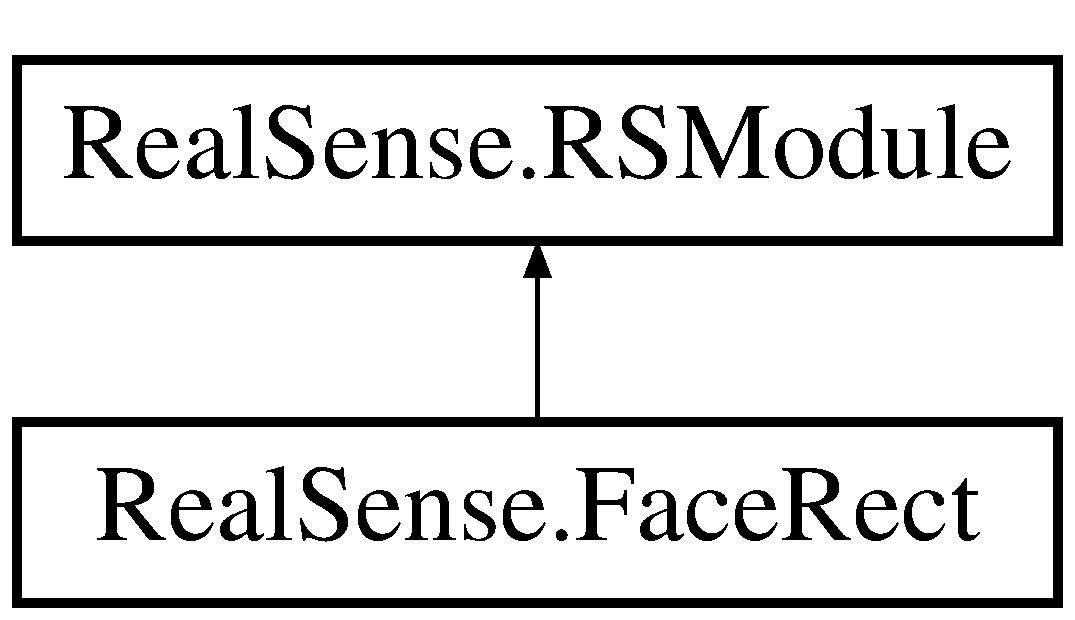
\includegraphics[height=2.000000cm]{class_real_sense_1_1_face_rect}
\end{center}
\end{figure}
\subsection*{Public Member Functions}
\begin{DoxyCompactItemize}
\item 
override void \hyperlink{class_real_sense_1_1_face_rect_aa2dbacb2ec8ac50b8fc19d02ceba2c0a}{Work} (Graphics g)
\end{DoxyCompactItemize}
\subsection*{Additional Inherited Members}


\subsection{Detailed Description}
Draws a rectangle, sorrounding the subject\textquotesingle{}s face \begin{DoxyAuthor}{Author}
\+: David Rosenbusch  Hufflepuff 
\end{DoxyAuthor}


Definition at line 15 of file Face\+Rect.\+cs.



\subsection{Member Function Documentation}
\mbox{\Hypertarget{class_real_sense_1_1_face_rect_aa2dbacb2ec8ac50b8fc19d02ceba2c0a}\label{class_real_sense_1_1_face_rect_aa2dbacb2ec8ac50b8fc19d02ceba2c0a}} 
\index{Real\+Sense\+::\+Face\+Rect@{Real\+Sense\+::\+Face\+Rect}!Work@{Work}}
\index{Work@{Work}!Real\+Sense\+::\+Face\+Rect@{Real\+Sense\+::\+Face\+Rect}}
\subsubsection{\texorpdfstring{Work()}{Work()}}
{\footnotesize\ttfamily override void Real\+Sense.\+Face\+Rect.\+Work (\begin{DoxyParamCaption}\item[{Graphics}]{g }\end{DoxyParamCaption})\hspace{0.3cm}{\ttfamily [virtual]}}

Draws a rectangle... wow 
\begin{DoxyParams}{Parameters}
{\em Graphics} & g for the view \\
\hline
\end{DoxyParams}


Implements \hyperlink{class_real_sense_1_1_r_s_module_a2ec830b7932ee7c0077d473f81c73867}{Real\+Sense.\+R\+S\+Module}.



Definition at line 23 of file Face\+Rect.\+cs.



The documentation for this class was generated from the following file\+:\begin{DoxyCompactItemize}
\item 
C\+:/\+Users/nutzer/\+Documents/\+Git\+Hub/\+Real\+Sense/\+Various/\hyperlink{_face_rect_8cs}{Face\+Rect.\+cs}\end{DoxyCompactItemize}

\hypertarget{class_real_sense_1_1_face_tracker_module}{}\section{Real\+Sense.\+Face\+Tracker\+Module Class Reference}
\label{class_real_sense_1_1_face_tracker_module}\index{Real\+Sense.\+Face\+Tracker\+Module@{Real\+Sense.\+Face\+Tracker\+Module}}
Inheritance diagram for Real\+Sense.\+Face\+Tracker\+Module\+:\begin{figure}[H]
\begin{center}
\leavevmode
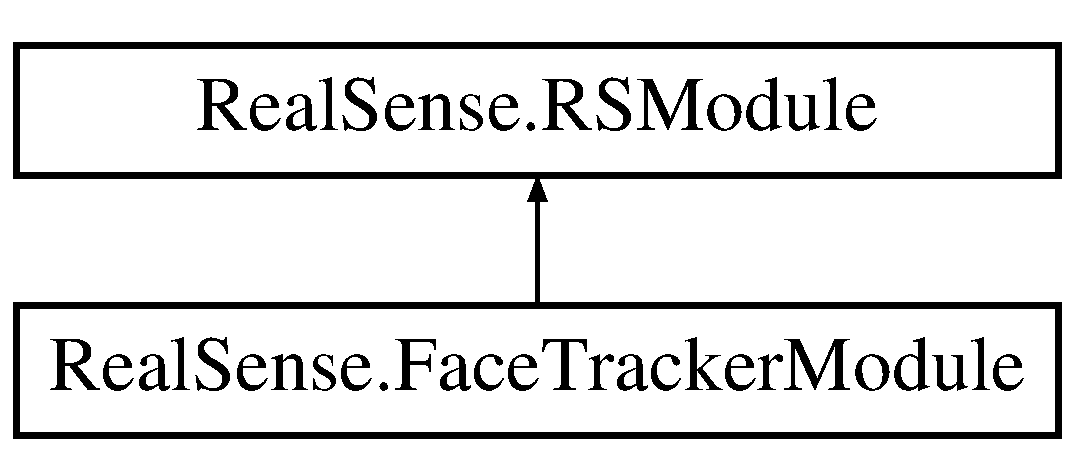
\includegraphics[height=2.000000cm]{class_real_sense_1_1_face_tracker_module}
\end{center}
\end{figure}
\subsection*{Public Member Functions}
\begin{DoxyCompactItemize}
\item 
\hyperlink{class_real_sense_1_1_face_tracker_module_ac34dc667e54a0a222f750f27f71734c4}{Face\+Tracker\+Module} (int\mbox{[}$\,$\mbox{]} idx)
\item 
override void \hyperlink{class_real_sense_1_1_face_tracker_module_a38b7097ab671999aae5f1a645fc623f8}{Work} (Graphics g)
\end{DoxyCompactItemize}
\subsection*{Additional Inherited Members}


\subsection{Detailed Description}


Definition at line 12 of file Face\+Tracker\+Module.\+cs.



\subsection{Constructor \& Destructor Documentation}
\mbox{\Hypertarget{class_real_sense_1_1_face_tracker_module_ac34dc667e54a0a222f750f27f71734c4}\label{class_real_sense_1_1_face_tracker_module_ac34dc667e54a0a222f750f27f71734c4}} 
\index{Real\+Sense\+::\+Face\+Tracker\+Module@{Real\+Sense\+::\+Face\+Tracker\+Module}!Face\+Tracker\+Module@{Face\+Tracker\+Module}}
\index{Face\+Tracker\+Module@{Face\+Tracker\+Module}!Real\+Sense\+::\+Face\+Tracker\+Module@{Real\+Sense\+::\+Face\+Tracker\+Module}}
\subsubsection{\texorpdfstring{Face\+Tracker\+Module()}{FaceTrackerModule()}}
{\footnotesize\ttfamily Real\+Sense.\+Face\+Tracker\+Module.\+Face\+Tracker\+Module (\begin{DoxyParamCaption}\item[{int \mbox{[}$\,$\mbox{]}}]{idx }\end{DoxyParamCaption})}



Definition at line 20 of file Face\+Tracker\+Module.\+cs.



\subsection{Member Function Documentation}
\mbox{\Hypertarget{class_real_sense_1_1_face_tracker_module_a38b7097ab671999aae5f1a645fc623f8}\label{class_real_sense_1_1_face_tracker_module_a38b7097ab671999aae5f1a645fc623f8}} 
\index{Real\+Sense\+::\+Face\+Tracker\+Module@{Real\+Sense\+::\+Face\+Tracker\+Module}!Work@{Work}}
\index{Work@{Work}!Real\+Sense\+::\+Face\+Tracker\+Module@{Real\+Sense\+::\+Face\+Tracker\+Module}}
\subsubsection{\texorpdfstring{Work()}{Work()}}
{\footnotesize\ttfamily override void Real\+Sense.\+Face\+Tracker\+Module.\+Work (\begin{DoxyParamCaption}\item[{Graphics}]{g }\end{DoxyParamCaption})\hspace{0.3cm}{\ttfamily [virtual]}}

Update every frame (do calculations, manipulate output Image) 
\begin{DoxyParams}{Parameters}
{\em Graphics} & g \\
\hline
\end{DoxyParams}


Implements \hyperlink{class_real_sense_1_1_r_s_module_a2ec830b7932ee7c0077d473f81c73867}{Real\+Sense.\+R\+S\+Module}.



Definition at line 25 of file Face\+Tracker\+Module.\+cs.



The documentation for this class was generated from the following file\+:\begin{DoxyCompactItemize}
\item 
Various/\hyperlink{_face_tracker_module_8cs}{Face\+Tracker\+Module.\+cs}\end{DoxyCompactItemize}

\hypertarget{class_real_sense_1_1_friggn_aweseome_graphix}{}\section{Real\+Sense.\+Friggn\+Aweseome\+Graphix Class Reference}
\label{class_real_sense_1_1_friggn_aweseome_graphix}\index{Real\+Sense.\+Friggn\+Aweseome\+Graphix@{Real\+Sense.\+Friggn\+Aweseome\+Graphix}}
\subsection*{Classes}
\begin{DoxyCompactItemize}
\item 
class \hyperlink{class_real_sense_1_1_friggn_aweseome_graphix_1_1_m_e_monitor}{M\+E\+Monitor}
\end{DoxyCompactItemize}
\subsection*{Static Public Member Functions}
\begin{DoxyCompactItemize}
\item 
static void \hyperlink{class_real_sense_1_1_friggn_aweseome_graphix_a9ebb178f63594b6b6dd9d650703de4d9}{Draw\+M\+E\+Montior} (Graphics gfx, \hyperlink{class_real_sense_1_1_friggn_aweseome_graphix_1_1_m_e_monitor}{M\+E\+Monitor} monitor)
\item 
static void \hyperlink{class_real_sense_1_1_friggn_aweseome_graphix_a79beae7f9b0458501156b023e3917d49}{Draw\+M\+E\+Montior} (Graphics gfx, \hyperlink{class_real_sense_1_1_friggn_aweseome_graphix_1_1_m_e_monitor}{M\+E\+Monitor} monitor, bool draw\+Text)
\item 
static unsafe void \hyperlink{class_real_sense_1_1_friggn_aweseome_graphix_a9e0391199c5b77e3153684deb2e30c5c}{Pretty\+\_\+blur} (Bitmap source, Bitmap target, int x0, int y0, int x1, int y1, int factor, Bitmap\+Data source\+Data, Bitmap\+Data target\+Data)
\item 
static unsafe void \hyperlink{class_real_sense_1_1_friggn_aweseome_graphix_aa9bd286dcff99c200fabc8368c9d41ff}{Sonic\+\_\+blur} (Bitmap source, Bitmap target, int x0, int y0, int x1, int y1, int factor, int channels, Bitmap\+Data source\+Data, Bitmap\+Data target\+Data)
\item 
static void \hyperlink{class_real_sense_1_1_friggn_aweseome_graphix_a213322f957a49429ac2a3017abdf49aa}{Draw\+Fading\+Line} (Graphics gfx, float x0, float y0, float x1, float y1)
\end{DoxyCompactItemize}
\subsection*{Static Public Attributes}
\begin{DoxyCompactItemize}
\item 
static Font \hyperlink{class_real_sense_1_1_friggn_aweseome_graphix_ad34adf2179722fa8080e9f4032bc43ce}{major\+Font} = new Font(\char`\"{}Futura\char`\"{}, 36, Font\+Style.\+Bold)
\item 
static Font \hyperlink{class_real_sense_1_1_friggn_aweseome_graphix_a9d2afacf158345fcecf1b25b895806a2}{minor\+Font} = new Font(\char`\"{}Futura\char`\"{}, 21, Font\+Style.\+Regular)
\item 
static Color \hyperlink{class_real_sense_1_1_friggn_aweseome_graphix_a167341ae00dc0a13928b8b26de77e277}{fg\+Color} = Color.\+From\+Argb(55, 186, 68, 75)
\item 
static Color \hyperlink{class_real_sense_1_1_friggn_aweseome_graphix_a80a40fcc2a193f1d3a2a7ba3d9d4eb2b}{font\+Color} = Color.\+From\+Argb(255, 103, 103, 104)
\end{DoxyCompactItemize}


\subsection{Detailed Description}
Includes some kickass graphics-\/stuff \begin{DoxyAuthor}{Author}
\+: David Rosenbusch  Hufflepuff 
\end{DoxyAuthor}


Definition at line 21 of file Friggn\+Aweseome\+Graphix.\+cs.



\subsection{Member Function Documentation}
\mbox{\Hypertarget{class_real_sense_1_1_friggn_aweseome_graphix_a213322f957a49429ac2a3017abdf49aa}\label{class_real_sense_1_1_friggn_aweseome_graphix_a213322f957a49429ac2a3017abdf49aa}} 
\index{Real\+Sense\+::\+Friggn\+Aweseome\+Graphix@{Real\+Sense\+::\+Friggn\+Aweseome\+Graphix}!Draw\+Fading\+Line@{Draw\+Fading\+Line}}
\index{Draw\+Fading\+Line@{Draw\+Fading\+Line}!Real\+Sense\+::\+Friggn\+Aweseome\+Graphix@{Real\+Sense\+::\+Friggn\+Aweseome\+Graphix}}
\subsubsection{\texorpdfstring{Draw\+Fading\+Line()}{DrawFadingLine()}}
{\footnotesize\ttfamily static void Real\+Sense.\+Friggn\+Aweseome\+Graphix.\+Draw\+Fading\+Line (\begin{DoxyParamCaption}\item[{Graphics}]{gfx,  }\item[{float}]{x0,  }\item[{float}]{y0,  }\item[{float}]{x1,  }\item[{float}]{y1 }\end{DoxyParamCaption})\hspace{0.3cm}{\ttfamily [static]}}

Draws a fading line (duh)


\begin{DoxyParams}{Parameters}
{\em Graphics} & gfx, graphics-\/object to draw on \\
\hline
{\em float} & x0, start x-\/coordinate \\
\hline
{\em float} & y0, start y-\/coordinate \\
\hline
{\em float} & x1, end x-\/coordinate \\
\hline
{\em float} & y1, end y-\/coordinate \\
\hline
\end{DoxyParams}


Definition at line 297 of file Friggn\+Aweseome\+Graphix.\+cs.

\mbox{\Hypertarget{class_real_sense_1_1_friggn_aweseome_graphix_a9ebb178f63594b6b6dd9d650703de4d9}\label{class_real_sense_1_1_friggn_aweseome_graphix_a9ebb178f63594b6b6dd9d650703de4d9}} 
\index{Real\+Sense\+::\+Friggn\+Aweseome\+Graphix@{Real\+Sense\+::\+Friggn\+Aweseome\+Graphix}!Draw\+M\+E\+Montior@{Draw\+M\+E\+Montior}}
\index{Draw\+M\+E\+Montior@{Draw\+M\+E\+Montior}!Real\+Sense\+::\+Friggn\+Aweseome\+Graphix@{Real\+Sense\+::\+Friggn\+Aweseome\+Graphix}}
\subsubsection{\texorpdfstring{Draw\+M\+E\+Montior()}{DrawMEMontior()}\hspace{0.1cm}{\footnotesize\ttfamily [1/2]}}
{\footnotesize\ttfamily static void Real\+Sense.\+Friggn\+Aweseome\+Graphix.\+Draw\+M\+E\+Montior (\begin{DoxyParamCaption}\item[{Graphics}]{gfx,  }\item[{\hyperlink{class_real_sense_1_1_friggn_aweseome_graphix_1_1_m_e_monitor}{M\+E\+Monitor}}]{monitor }\end{DoxyParamCaption})\hspace{0.3cm}{\ttfamily [static]}}

Draws a M\+E\+Montior ontop of the graphics-\/object. Displays text as per default.


\begin{DoxyParams}{Parameters}
{\em Graphics} & gfx, graphics-\/object to draw Monitor on \\
\hline
{\em \hyperlink{class_real_sense_1_1_friggn_aweseome_graphix_1_1_m_e_monitor}{M\+E\+Monitor}} & monitor, monitor to be drawn \\
\hline
\end{DoxyParams}


Definition at line 88 of file Friggn\+Aweseome\+Graphix.\+cs.

\mbox{\Hypertarget{class_real_sense_1_1_friggn_aweseome_graphix_a79beae7f9b0458501156b023e3917d49}\label{class_real_sense_1_1_friggn_aweseome_graphix_a79beae7f9b0458501156b023e3917d49}} 
\index{Real\+Sense\+::\+Friggn\+Aweseome\+Graphix@{Real\+Sense\+::\+Friggn\+Aweseome\+Graphix}!Draw\+M\+E\+Montior@{Draw\+M\+E\+Montior}}
\index{Draw\+M\+E\+Montior@{Draw\+M\+E\+Montior}!Real\+Sense\+::\+Friggn\+Aweseome\+Graphix@{Real\+Sense\+::\+Friggn\+Aweseome\+Graphix}}
\subsubsection{\texorpdfstring{Draw\+M\+E\+Montior()}{DrawMEMontior()}\hspace{0.1cm}{\footnotesize\ttfamily [2/2]}}
{\footnotesize\ttfamily static void Real\+Sense.\+Friggn\+Aweseome\+Graphix.\+Draw\+M\+E\+Montior (\begin{DoxyParamCaption}\item[{Graphics}]{gfx,  }\item[{\hyperlink{class_real_sense_1_1_friggn_aweseome_graphix_1_1_m_e_monitor}{M\+E\+Monitor}}]{monitor,  }\item[{bool}]{draw\+Text }\end{DoxyParamCaption})\hspace{0.3cm}{\ttfamily [static]}}

Draws a M\+E\+Montior ontop of the graphics-\/object. Displays text as per default.


\begin{DoxyParams}{Parameters}
{\em Graphics} & gfx, graphics-\/object to draw Monitor on \\
\hline
{\em \hyperlink{class_real_sense_1_1_friggn_aweseome_graphix_1_1_m_e_monitor}{M\+E\+Monitor}} & monitor, monitor to be drawn \\
\hline
{\em bool} & draw\+Text, flag to display value as text (or not) \\
\hline
\end{DoxyParams}


Definition at line 98 of file Friggn\+Aweseome\+Graphix.\+cs.

\mbox{\Hypertarget{class_real_sense_1_1_friggn_aweseome_graphix_a9e0391199c5b77e3153684deb2e30c5c}\label{class_real_sense_1_1_friggn_aweseome_graphix_a9e0391199c5b77e3153684deb2e30c5c}} 
\index{Real\+Sense\+::\+Friggn\+Aweseome\+Graphix@{Real\+Sense\+::\+Friggn\+Aweseome\+Graphix}!Pretty\+\_\+blur@{Pretty\+\_\+blur}}
\index{Pretty\+\_\+blur@{Pretty\+\_\+blur}!Real\+Sense\+::\+Friggn\+Aweseome\+Graphix@{Real\+Sense\+::\+Friggn\+Aweseome\+Graphix}}
\subsubsection{\texorpdfstring{Pretty\+\_\+blur()}{Pretty\_blur()}}
{\footnotesize\ttfamily static unsafe void Real\+Sense.\+Friggn\+Aweseome\+Graphix.\+Pretty\+\_\+blur (\begin{DoxyParamCaption}\item[{Bitmap}]{source,  }\item[{Bitmap}]{target,  }\item[{int}]{x0,  }\item[{int}]{y0,  }\item[{int}]{x1,  }\item[{int}]{y1,  }\item[{int}]{factor,  }\item[{Bitmap\+Data}]{source\+Data,  }\item[{Bitmap\+Data}]{target\+Data }\end{DoxyParamCaption})\hspace{0.3cm}{\ttfamily [static]}}

\subparagraph*{}

\subsection*{Graphics}

\subparagraph*{}

Blurs an image and saves result in a new Bitmap Slow, but mathematically correct 
\begin{DoxyParams}{Parameters}
{\em Bitmap} & source -\/ original image, which is supposed to be blurred \\
\hline
{\em Bitmap} & target -\/ will contain the new image \\
\hline
{\em int} & x0 -\/ upper-\/left x-\/coordinate of area that is supposed to be blurred \\
\hline
{\em int} & y0 -\/ upper-\/left y-\/coordinate of area that is supposed to be blurred \\
\hline
{\em int} & x1 -\/ lower-\/right x-\/coordinate of area that is supposed to be blurred \\
\hline
{\em int} & y1 -\/ lower-\/right y-\/coordinate of area that is supposed to be blurred \\
\hline
{\em factor} & -\/ blur\+Factor \\
\hline
{\em Bitmap\+Data} & source\+Data -\/ data of original image \\
\hline
{\em Bitmap\+Data} & source\+Data -\/ data of target image \\
\hline
\end{DoxyParams}


Definition at line 144 of file Friggn\+Aweseome\+Graphix.\+cs.

\mbox{\Hypertarget{class_real_sense_1_1_friggn_aweseome_graphix_aa9bd286dcff99c200fabc8368c9d41ff}\label{class_real_sense_1_1_friggn_aweseome_graphix_aa9bd286dcff99c200fabc8368c9d41ff}} 
\index{Real\+Sense\+::\+Friggn\+Aweseome\+Graphix@{Real\+Sense\+::\+Friggn\+Aweseome\+Graphix}!Sonic\+\_\+blur@{Sonic\+\_\+blur}}
\index{Sonic\+\_\+blur@{Sonic\+\_\+blur}!Real\+Sense\+::\+Friggn\+Aweseome\+Graphix@{Real\+Sense\+::\+Friggn\+Aweseome\+Graphix}}
\subsubsection{\texorpdfstring{Sonic\+\_\+blur()}{Sonic\_blur()}}
{\footnotesize\ttfamily static unsafe void Real\+Sense.\+Friggn\+Aweseome\+Graphix.\+Sonic\+\_\+blur (\begin{DoxyParamCaption}\item[{Bitmap}]{source,  }\item[{Bitmap}]{target,  }\item[{int}]{x0,  }\item[{int}]{y0,  }\item[{int}]{x1,  }\item[{int}]{y1,  }\item[{int}]{factor,  }\item[{int}]{channels,  }\item[{Bitmap\+Data}]{source\+Data,  }\item[{Bitmap\+Data}]{target\+Data }\end{DoxyParamCaption})\hspace{0.3cm}{\ttfamily [static]}}

Blurs an image and saves result in a new Bitmap Faster, but mathematically incorrect 
\begin{DoxyParams}{Parameters}
{\em Bitmap} & source -\/ original image, which is supposed to be blurred \\
\hline
{\em Bitmap} & target -\/ will contain the new image \\
\hline
{\em int} & x0 -\/ upper-\/left x-\/coordinate of area that is supposed to be blurred \\
\hline
{\em int} & y0 -\/ upper-\/left y-\/coordinate of area that is supposed to be blurred \\
\hline
{\em int} & x1 -\/ lower-\/right x-\/coordinate of area that is supposed to be blurred \\
\hline
{\em int} & y1 -\/ lower-\/right y-\/coordinate of area that is supposed to be blurred \\
\hline
{\em factor} & -\/ blur\+Factor \\
\hline
{\em channels} & -\/ number of color-\/channels \\
\hline
{\em Bitmap\+Data} & source\+Data -\/ data of original image \\
\hline
{\em Bitmap\+Data} & source\+Data -\/ data of target image \\
\hline
\end{DoxyParams}


Definition at line 224 of file Friggn\+Aweseome\+Graphix.\+cs.



\subsection{Member Data Documentation}
\mbox{\Hypertarget{class_real_sense_1_1_friggn_aweseome_graphix_a167341ae00dc0a13928b8b26de77e277}\label{class_real_sense_1_1_friggn_aweseome_graphix_a167341ae00dc0a13928b8b26de77e277}} 
\index{Real\+Sense\+::\+Friggn\+Aweseome\+Graphix@{Real\+Sense\+::\+Friggn\+Aweseome\+Graphix}!fg\+Color@{fg\+Color}}
\index{fg\+Color@{fg\+Color}!Real\+Sense\+::\+Friggn\+Aweseome\+Graphix@{Real\+Sense\+::\+Friggn\+Aweseome\+Graphix}}
\subsubsection{\texorpdfstring{fg\+Color}{fgColor}}
{\footnotesize\ttfamily Color Real\+Sense.\+Friggn\+Aweseome\+Graphix.\+fg\+Color = Color.\+From\+Argb(55, 186, 68, 75)\hspace{0.3cm}{\ttfamily [static]}}



Definition at line 34 of file Friggn\+Aweseome\+Graphix.\+cs.

\mbox{\Hypertarget{class_real_sense_1_1_friggn_aweseome_graphix_a80a40fcc2a193f1d3a2a7ba3d9d4eb2b}\label{class_real_sense_1_1_friggn_aweseome_graphix_a80a40fcc2a193f1d3a2a7ba3d9d4eb2b}} 
\index{Real\+Sense\+::\+Friggn\+Aweseome\+Graphix@{Real\+Sense\+::\+Friggn\+Aweseome\+Graphix}!font\+Color@{font\+Color}}
\index{font\+Color@{font\+Color}!Real\+Sense\+::\+Friggn\+Aweseome\+Graphix@{Real\+Sense\+::\+Friggn\+Aweseome\+Graphix}}
\subsubsection{\texorpdfstring{font\+Color}{fontColor}}
{\footnotesize\ttfamily Color Real\+Sense.\+Friggn\+Aweseome\+Graphix.\+font\+Color = Color.\+From\+Argb(255, 103, 103, 104)\hspace{0.3cm}{\ttfamily [static]}}



Definition at line 36 of file Friggn\+Aweseome\+Graphix.\+cs.

\mbox{\Hypertarget{class_real_sense_1_1_friggn_aweseome_graphix_ad34adf2179722fa8080e9f4032bc43ce}\label{class_real_sense_1_1_friggn_aweseome_graphix_ad34adf2179722fa8080e9f4032bc43ce}} 
\index{Real\+Sense\+::\+Friggn\+Aweseome\+Graphix@{Real\+Sense\+::\+Friggn\+Aweseome\+Graphix}!major\+Font@{major\+Font}}
\index{major\+Font@{major\+Font}!Real\+Sense\+::\+Friggn\+Aweseome\+Graphix@{Real\+Sense\+::\+Friggn\+Aweseome\+Graphix}}
\subsubsection{\texorpdfstring{major\+Font}{majorFont}}
{\footnotesize\ttfamily Font Real\+Sense.\+Friggn\+Aweseome\+Graphix.\+major\+Font = new Font(\char`\"{}Futura\char`\"{}, 36, Font\+Style.\+Bold)\hspace{0.3cm}{\ttfamily [static]}}



Definition at line 32 of file Friggn\+Aweseome\+Graphix.\+cs.

\mbox{\Hypertarget{class_real_sense_1_1_friggn_aweseome_graphix_a9d2afacf158345fcecf1b25b895806a2}\label{class_real_sense_1_1_friggn_aweseome_graphix_a9d2afacf158345fcecf1b25b895806a2}} 
\index{Real\+Sense\+::\+Friggn\+Aweseome\+Graphix@{Real\+Sense\+::\+Friggn\+Aweseome\+Graphix}!minor\+Font@{minor\+Font}}
\index{minor\+Font@{minor\+Font}!Real\+Sense\+::\+Friggn\+Aweseome\+Graphix@{Real\+Sense\+::\+Friggn\+Aweseome\+Graphix}}
\subsubsection{\texorpdfstring{minor\+Font}{minorFont}}
{\footnotesize\ttfamily Font Real\+Sense.\+Friggn\+Aweseome\+Graphix.\+minor\+Font = new Font(\char`\"{}Futura\char`\"{}, 21, Font\+Style.\+Regular)\hspace{0.3cm}{\ttfamily [static]}}



Definition at line 33 of file Friggn\+Aweseome\+Graphix.\+cs.



The documentation for this class was generated from the following file\+:\begin{DoxyCompactItemize}
\item 
C\+:/\+Users/nutzer/\+Documents/\+Git\+Hub/\+Real\+Sense/\+Framework/\hyperlink{_friggn_aweseome_graphix_8cs}{Friggn\+Aweseome\+Graphix.\+cs}\end{DoxyCompactItemize}

\hypertarget{class_real_sense_1_1_gauge___module}{}\section{Real\+Sense.\+Gauge\+\_\+\+Module Class Reference}
\label{class_real_sense_1_1_gauge___module}\index{Real\+Sense.\+Gauge\+\_\+\+Module@{Real\+Sense.\+Gauge\+\_\+\+Module}}
Inheritance diagram for Real\+Sense.\+Gauge\+\_\+\+Module\+:\begin{figure}[H]
\begin{center}
\leavevmode
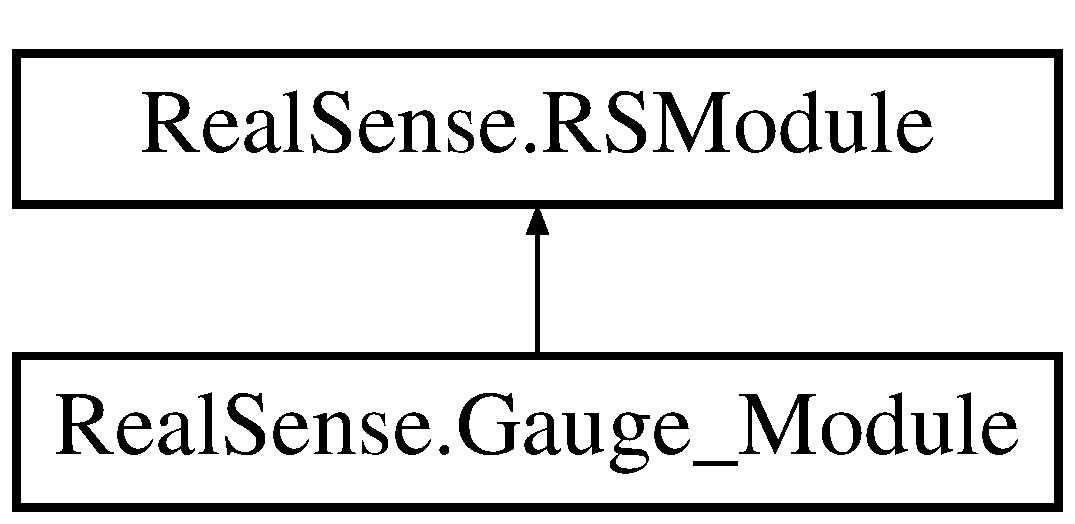
\includegraphics[height=2.000000cm]{class_real_sense_1_1_gauge___module}
\end{center}
\end{figure}
\subsection*{Public Member Functions}
\begin{DoxyCompactItemize}
\item 
void \hyperlink{class_real_sense_1_1_gauge___module_a367111d614ea2a05af81e93a3b957cd4}{Update} ()
\item 
override void \hyperlink{class_real_sense_1_1_gauge___module_a587ea68ad539f2f56bcfbd7641a92a83}{Work} (Graphics g)
\end{DoxyCompactItemize}
\subsection*{Public Attributes}
\begin{DoxyCompactItemize}
\item 
bool \hyperlink{class_real_sense_1_1_gauge___module_a116882e1610b28a8ce6159b1ddbbf578}{calibrate} = false
\item 
bool \hyperlink{class_real_sense_1_1_gauge___module_ae9d8d183234958600957fdfd23c4d850}{frame\+Update} = true
\end{DoxyCompactItemize}
\subsection*{Additional Inherited Members}


\subsection{Detailed Description}
Module used to calibrate the user\textquotesingle{}s nullface by averaging over a set amount of frames (num\+Faces)

\begin{DoxyAuthor}{Author}
\+: David Rosenbusch  Hufflepuff 
\end{DoxyAuthor}


Definition at line 20 of file Gauge\+\_\+\+Module.\+cs.



\subsection{Member Function Documentation}
\mbox{\Hypertarget{class_real_sense_1_1_gauge___module_a367111d614ea2a05af81e93a3b957cd4}\label{class_real_sense_1_1_gauge___module_a367111d614ea2a05af81e93a3b957cd4}} 
\index{Real\+Sense\+::\+Gauge\+\_\+\+Module@{Real\+Sense\+::\+Gauge\+\_\+\+Module}!Update@{Update}}
\index{Update@{Update}!Real\+Sense\+::\+Gauge\+\_\+\+Module@{Real\+Sense\+::\+Gauge\+\_\+\+Module}}
\subsubsection{\texorpdfstring{Update()}{Update()}}
{\footnotesize\ttfamily void Real\+Sense.\+Gauge\+\_\+\+Module.\+Update (\begin{DoxyParamCaption}{ }\end{DoxyParamCaption})}

Gathers calibration-\/data. When a new frame is shot A\+ND still calibrating (button was pressed), adds a new face to the Filtered\+Avg. After having num\+Faces faces, calculate... Runs outside the Camera Thread 

Definition at line 62 of file Gauge\+\_\+\+Module.\+cs.

\mbox{\Hypertarget{class_real_sense_1_1_gauge___module_a587ea68ad539f2f56bcfbd7641a92a83}\label{class_real_sense_1_1_gauge___module_a587ea68ad539f2f56bcfbd7641a92a83}} 
\index{Real\+Sense\+::\+Gauge\+\_\+\+Module@{Real\+Sense\+::\+Gauge\+\_\+\+Module}!Work@{Work}}
\index{Work@{Work}!Real\+Sense\+::\+Gauge\+\_\+\+Module@{Real\+Sense\+::\+Gauge\+\_\+\+Module}}
\subsubsection{\texorpdfstring{Work()}{Work()}}
{\footnotesize\ttfamily override void Real\+Sense.\+Gauge\+\_\+\+Module.\+Work (\begin{DoxyParamCaption}\item[{Graphics}]{g }\end{DoxyParamCaption})\hspace{0.3cm}{\ttfamily [virtual]}}

Update every frame (do calculations, manipulate output Image) 
\begin{DoxyParams}{Parameters}
{\em Graphics} & g \\
\hline
\end{DoxyParams}


Implements \hyperlink{class_real_sense_1_1_r_s_module_a2ec830b7932ee7c0077d473f81c73867}{Real\+Sense.\+R\+S\+Module}.



Definition at line 133 of file Gauge\+\_\+\+Module.\+cs.



\subsection{Member Data Documentation}
\mbox{\Hypertarget{class_real_sense_1_1_gauge___module_a116882e1610b28a8ce6159b1ddbbf578}\label{class_real_sense_1_1_gauge___module_a116882e1610b28a8ce6159b1ddbbf578}} 
\index{Real\+Sense\+::\+Gauge\+\_\+\+Module@{Real\+Sense\+::\+Gauge\+\_\+\+Module}!calibrate@{calibrate}}
\index{calibrate@{calibrate}!Real\+Sense\+::\+Gauge\+\_\+\+Module@{Real\+Sense\+::\+Gauge\+\_\+\+Module}}
\subsubsection{\texorpdfstring{calibrate}{calibrate}}
{\footnotesize\ttfamily bool Real\+Sense.\+Gauge\+\_\+\+Module.\+calibrate = false}



Definition at line 23 of file Gauge\+\_\+\+Module.\+cs.

\mbox{\Hypertarget{class_real_sense_1_1_gauge___module_ae9d8d183234958600957fdfd23c4d850}\label{class_real_sense_1_1_gauge___module_ae9d8d183234958600957fdfd23c4d850}} 
\index{Real\+Sense\+::\+Gauge\+\_\+\+Module@{Real\+Sense\+::\+Gauge\+\_\+\+Module}!frame\+Update@{frame\+Update}}
\index{frame\+Update@{frame\+Update}!Real\+Sense\+::\+Gauge\+\_\+\+Module@{Real\+Sense\+::\+Gauge\+\_\+\+Module}}
\subsubsection{\texorpdfstring{frame\+Update}{frameUpdate}}
{\footnotesize\ttfamily bool Real\+Sense.\+Gauge\+\_\+\+Module.\+frame\+Update = true}



Definition at line 31 of file Gauge\+\_\+\+Module.\+cs.



The documentation for this class was generated from the following file\+:\begin{DoxyCompactItemize}
\item 
Various/\hyperlink{_gauge___module_8cs}{Gauge\+\_\+\+Module.\+cs}\end{DoxyCompactItemize}

\section{Real\+Sense.\+Landmark\+Group\+Module Class Reference}
\label{class_real_sense_1_1_landmark_group_module}\index{Real\+Sense.\+Landmark\+Group\+Module@{Real\+Sense.\+Landmark\+Group\+Module}}
Inheritance diagram for Real\+Sense.\+Landmark\+Group\+Module\+:\begin{figure}[H]
\begin{center}
\leavevmode
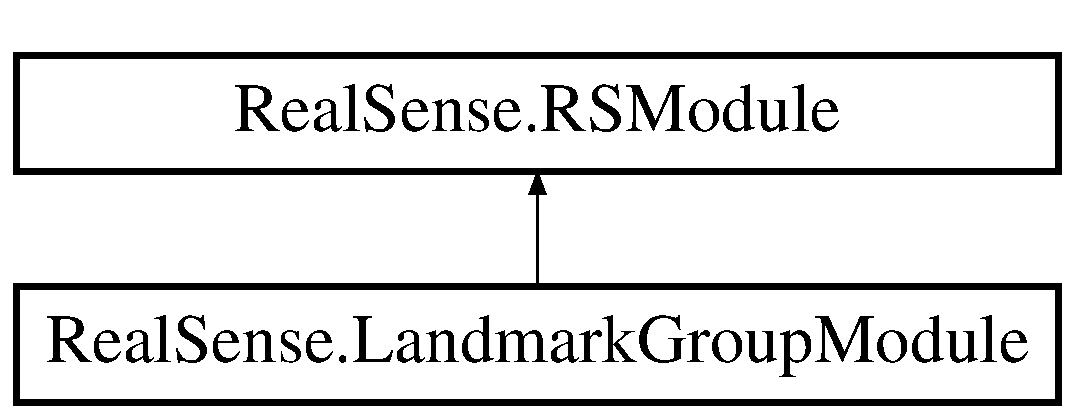
\includegraphics[height=2.000000cm]{class_real_sense_1_1_landmark_group_module}
\end{center}
\end{figure}
\subsection*{Public Member Functions}
\begin{DoxyCompactItemize}
\item 
override void \textbf{ Work} (Graphics g)
\end{DoxyCompactItemize}
\subsection*{Additional Inherited Members}


\subsection{Detailed Description}
Module to display Landmark-\/\+Points by their groups, as they are defined in the S\+DK \begin{DoxyAuthor}{Author}
\+: David Rosenbusch 

\+: Tobias Schramm  Hufflepuff 
\end{DoxyAuthor}


\subsection{Member Function Documentation}
\mbox{\label{class_real_sense_1_1_landmark_group_module_aae68525cdcf843719e02fa9b7317d3fa}} 
\index{Real\+Sense\+::\+Landmark\+Group\+Module@{Real\+Sense\+::\+Landmark\+Group\+Module}!Work@{Work}}
\index{Work@{Work}!Real\+Sense\+::\+Landmark\+Group\+Module@{Real\+Sense\+::\+Landmark\+Group\+Module}}
\subsubsection{Work()}
{\footnotesize\ttfamily override void Real\+Sense.\+Landmark\+Group\+Module.\+Work (\begin{DoxyParamCaption}\item[{Graphics}]{g }\end{DoxyParamCaption})\hspace{0.3cm}{\ttfamily [virtual]}}

Displays Landmarks by group, as they are defined in the S\+DK 
\begin{DoxyParams}{Parameters}
{\em Graphics} & g for the view \\
\hline
\end{DoxyParams}


Implements \textbf{ Real\+Sense.\+R\+S\+Module} \doxyref{}{p.}{class_real_sense_1_1_r_s_module_a2ec830b7932ee7c0077d473f81c73867}.



The documentation for this class was generated from the following file\+:\begin{DoxyCompactItemize}
\item 
Various/\textbf{ Landmark\+Group\+Module.\+cs}\end{DoxyCompactItemize}

\hypertarget{class_real_sense_1_1_landmark_type_module}{}\section{Real\+Sense.\+Landmark\+Type\+Module Class Reference}
\label{class_real_sense_1_1_landmark_type_module}\index{Real\+Sense.\+Landmark\+Type\+Module@{Real\+Sense.\+Landmark\+Type\+Module}}
Inheritance diagram for Real\+Sense.\+Landmark\+Type\+Module\+:\begin{figure}[H]
\begin{center}
\leavevmode
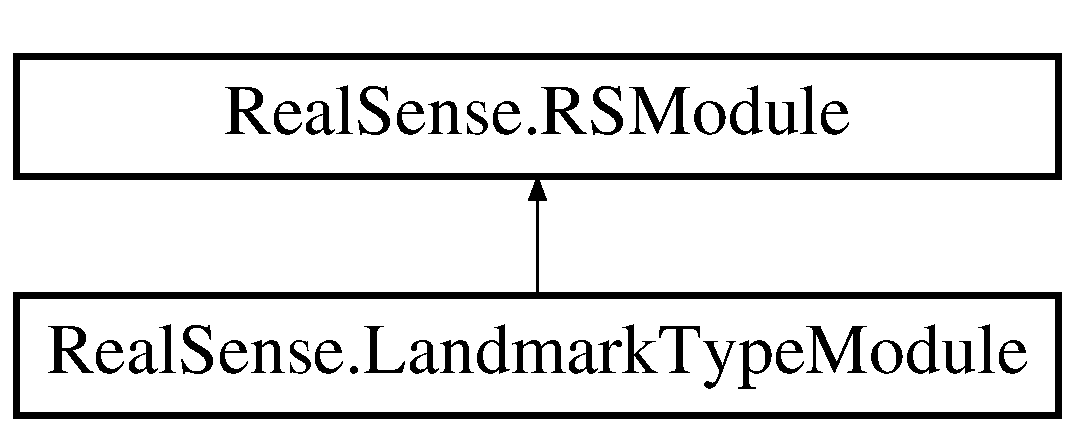
\includegraphics[height=2.000000cm]{class_real_sense_1_1_landmark_type_module}
\end{center}
\end{figure}
\subsection*{Public Member Functions}
\begin{DoxyCompactItemize}
\item 
override void \hyperlink{class_real_sense_1_1_landmark_type_module_ad110598b840e5496c1539862c4c53bc7}{Work} (Graphics g)
\end{DoxyCompactItemize}
\subsection*{Additional Inherited Members}


\subsection{Detailed Description}


Definition at line 13 of file Landmark\+Type\+Module.\+cs.



\subsection{Member Function Documentation}
\mbox{\Hypertarget{class_real_sense_1_1_landmark_type_module_ad110598b840e5496c1539862c4c53bc7}\label{class_real_sense_1_1_landmark_type_module_ad110598b840e5496c1539862c4c53bc7}} 
\index{Real\+Sense\+::\+Landmark\+Type\+Module@{Real\+Sense\+::\+Landmark\+Type\+Module}!Work@{Work}}
\index{Work@{Work}!Real\+Sense\+::\+Landmark\+Type\+Module@{Real\+Sense\+::\+Landmark\+Type\+Module}}
\subsubsection{\texorpdfstring{Work()}{Work()}}
{\footnotesize\ttfamily override void Real\+Sense.\+Landmark\+Type\+Module.\+Work (\begin{DoxyParamCaption}\item[{Graphics}]{g }\end{DoxyParamCaption})\hspace{0.3cm}{\ttfamily [virtual]}}

Update every frame (do calculations, manipulate output Image) 
\begin{DoxyParams}{Parameters}
{\em Graphics} & g \\
\hline
\end{DoxyParams}


Implements \hyperlink{class_real_sense_1_1_r_s_module_a2ec830b7932ee7c0077d473f81c73867}{Real\+Sense.\+R\+S\+Module}.



Definition at line 44 of file Landmark\+Type\+Module.\+cs.



The documentation for this class was generated from the following file\+:\begin{DoxyCompactItemize}
\item 
Various/\hyperlink{_landmark_type_module_8cs}{Landmark\+Type\+Module.\+cs}\end{DoxyCompactItemize}

\hypertarget{class_real_sense_1_1_m_e___bear_teeth}{}\section{Real\+Sense.\+M\+E\+\_\+\+Bear\+Teeth Class Reference}
\label{class_real_sense_1_1_m_e___bear_teeth}\index{Real\+Sense.\+M\+E\+\_\+\+Bear\+Teeth@{Real\+Sense.\+M\+E\+\_\+\+Bear\+Teeth}}
Inheritance diagram for Real\+Sense.\+M\+E\+\_\+\+Bear\+Teeth\+:\begin{figure}[H]
\begin{center}
\leavevmode
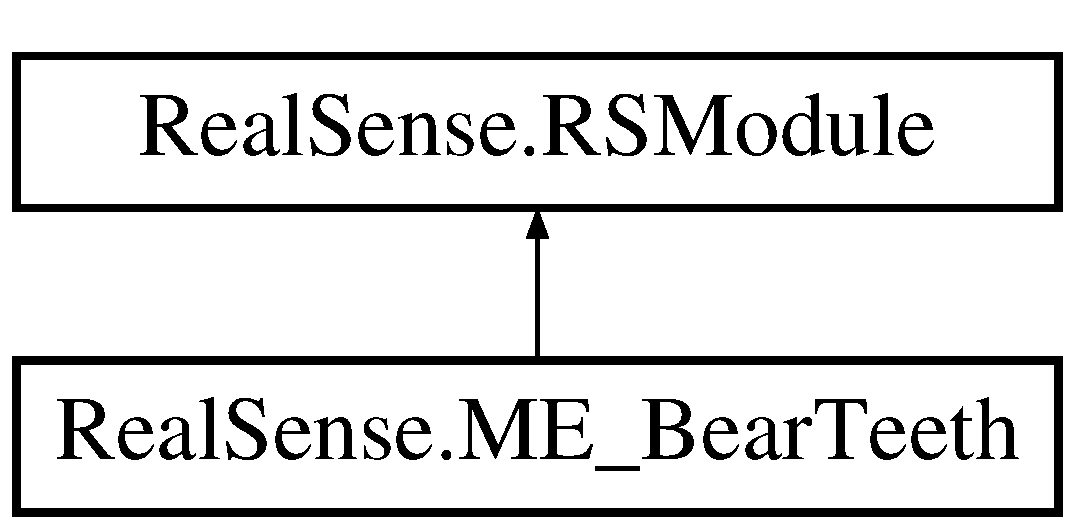
\includegraphics[height=2.000000cm]{class_real_sense_1_1_m_e___bear_teeth}
\end{center}
\end{figure}
\subsection*{Public Member Functions}
\begin{DoxyCompactItemize}
\item 
\hyperlink{class_real_sense_1_1_m_e___bear_teeth_a3500b0821cc64ae9909c1f273c1121f0}{M\+E\+\_\+\+Bear\+Teeth} ()
\item 
override void \hyperlink{class_real_sense_1_1_m_e___bear_teeth_a2e4cc340fec3499318fa7514ee7f1822}{Work} (Graphics g)
\end{DoxyCompactItemize}
\subsection*{Additional Inherited Members}


\subsection{Detailed Description}


Definition at line 9 of file M\+E\+\_\+\+Bear\+Teeth.\+cs.



\subsection{Constructor \& Destructor Documentation}
\mbox{\Hypertarget{class_real_sense_1_1_m_e___bear_teeth_a3500b0821cc64ae9909c1f273c1121f0}\label{class_real_sense_1_1_m_e___bear_teeth_a3500b0821cc64ae9909c1f273c1121f0}} 
\index{Real\+Sense\+::\+M\+E\+\_\+\+Bear\+Teeth@{Real\+Sense\+::\+M\+E\+\_\+\+Bear\+Teeth}!M\+E\+\_\+\+Bear\+Teeth@{M\+E\+\_\+\+Bear\+Teeth}}
\index{M\+E\+\_\+\+Bear\+Teeth@{M\+E\+\_\+\+Bear\+Teeth}!Real\+Sense\+::\+M\+E\+\_\+\+Bear\+Teeth@{Real\+Sense\+::\+M\+E\+\_\+\+Bear\+Teeth}}
\subsubsection{\texorpdfstring{M\+E\+\_\+\+Bear\+Teeth()}{ME\_BearTeeth()}}
{\footnotesize\ttfamily Real\+Sense.\+M\+E\+\_\+\+Bear\+Teeth.\+M\+E\+\_\+\+Bear\+Teeth (\begin{DoxyParamCaption}{ }\end{DoxyParamCaption})}

Sets default-\/values 

Definition at line 22 of file M\+E\+\_\+\+Bear\+Teeth.\+cs.



\subsection{Member Function Documentation}
\mbox{\Hypertarget{class_real_sense_1_1_m_e___bear_teeth_a2e4cc340fec3499318fa7514ee7f1822}\label{class_real_sense_1_1_m_e___bear_teeth_a2e4cc340fec3499318fa7514ee7f1822}} 
\index{Real\+Sense\+::\+M\+E\+\_\+\+Bear\+Teeth@{Real\+Sense\+::\+M\+E\+\_\+\+Bear\+Teeth}!Work@{Work}}
\index{Work@{Work}!Real\+Sense\+::\+M\+E\+\_\+\+Bear\+Teeth@{Real\+Sense\+::\+M\+E\+\_\+\+Bear\+Teeth}}
\subsubsection{\texorpdfstring{Work()}{Work()}}
{\footnotesize\ttfamily override void Real\+Sense.\+M\+E\+\_\+\+Bear\+Teeth.\+Work (\begin{DoxyParamCaption}\item[{Graphics}]{g }\end{DoxyParamCaption})\hspace{0.3cm}{\ttfamily [virtual]}}

Calculates the difference between the two lip corners 

Implements \hyperlink{class_real_sense_1_1_r_s_module_a2ec830b7932ee7c0077d473f81c73867}{Real\+Sense.\+R\+S\+Module}.



Definition at line 39 of file M\+E\+\_\+\+Bear\+Teeth.\+cs.



The documentation for this class was generated from the following file\+:\begin{DoxyCompactItemize}
\item 
Various/\hyperlink{_m_e___bear_teeth_8cs}{M\+E\+\_\+\+Bear\+Teeth.\+cs}\end{DoxyCompactItemize}

\hypertarget{class_real_sense_1_1_friggn_aweseome_graphix_1_1_m_e_monitor}{}\section{Real\+Sense.\+Friggn\+Aweseome\+Graphix.\+M\+E\+Monitor Class Reference}
\label{class_real_sense_1_1_friggn_aweseome_graphix_1_1_m_e_monitor}\index{Real\+Sense.\+Friggn\+Aweseome\+Graphix.\+M\+E\+Monitor@{Real\+Sense.\+Friggn\+Aweseome\+Graphix.\+M\+E\+Monitor}}
\subsection*{Public Member Functions}
\begin{DoxyCompactItemize}
\item 
\hyperlink{class_real_sense_1_1_friggn_aweseome_graphix_1_1_m_e_monitor_a8df7ffb411949e73cc37344326d325a3}{M\+E\+Monitor} (String maj\+Text, String min\+Text, int xP, int yP, int rad, int thick)
\item 
void \hyperlink{class_real_sense_1_1_friggn_aweseome_graphix_1_1_m_e_monitor_aa55989a875d2fd83969adb5388c691f1}{Step} ()
\end{DoxyCompactItemize}
\subsection*{Public Attributes}
\begin{DoxyCompactItemize}
\item 
int \hyperlink{class_real_sense_1_1_friggn_aweseome_graphix_1_1_m_e_monitor_aae94a9af9eba40d10677cffeee537737}{x}
\item 
int \hyperlink{class_real_sense_1_1_friggn_aweseome_graphix_1_1_m_e_monitor_a05c8b06b952fbdfff729f92498996212}{y}
\item 
int \hyperlink{class_real_sense_1_1_friggn_aweseome_graphix_1_1_m_e_monitor_aac6a6a6847e001a75e2b2316386ee864}{radius}
\item 
int \hyperlink{class_real_sense_1_1_friggn_aweseome_graphix_1_1_m_e_monitor_abb4069ab5c96cb77807c8ec988073bb0}{thickness}
\item 
int \hyperlink{class_real_sense_1_1_friggn_aweseome_graphix_1_1_m_e_monitor_adc8792c41789b6f038d7dc5d5c6e7496}{current\+Value} = 0
\item 
int \hyperlink{class_real_sense_1_1_friggn_aweseome_graphix_1_1_m_e_monitor_aa73071b1e565f6765783baf18ce5b2c7}{target\+Value} = 0
\item 
String \hyperlink{class_real_sense_1_1_friggn_aweseome_graphix_1_1_m_e_monitor_a4cdd7aad6b3e84b9429518891618b195}{major\+Text}
\item 
String \hyperlink{class_real_sense_1_1_friggn_aweseome_graphix_1_1_m_e_monitor_a6bbf9a1ee06067597b933da3e34e3ee5}{minor\+Text}
\item 
bool \hyperlink{class_real_sense_1_1_friggn_aweseome_graphix_1_1_m_e_monitor_a4a07682a2e90f7433ae6fdb9df8f9b97}{show\+Percent} = true
\end{DoxyCompactItemize}


\subsection{Detailed Description}
Custom U\+I-\/\+Component to stylishly display percentage-\/values 

Definition at line 41 of file Friggn\+Aweseome\+Graphix.\+cs.



\subsection{Constructor \& Destructor Documentation}
\mbox{\Hypertarget{class_real_sense_1_1_friggn_aweseome_graphix_1_1_m_e_monitor_a8df7ffb411949e73cc37344326d325a3}\label{class_real_sense_1_1_friggn_aweseome_graphix_1_1_m_e_monitor_a8df7ffb411949e73cc37344326d325a3}} 
\index{Real\+Sense\+::\+Friggn\+Aweseome\+Graphix\+::\+M\+E\+Monitor@{Real\+Sense\+::\+Friggn\+Aweseome\+Graphix\+::\+M\+E\+Monitor}!M\+E\+Monitor@{M\+E\+Monitor}}
\index{M\+E\+Monitor@{M\+E\+Monitor}!Real\+Sense\+::\+Friggn\+Aweseome\+Graphix\+::\+M\+E\+Monitor@{Real\+Sense\+::\+Friggn\+Aweseome\+Graphix\+::\+M\+E\+Monitor}}
\subsubsection{\texorpdfstring{M\+E\+Monitor()}{MEMonitor()}}
{\footnotesize\ttfamily Real\+Sense.\+Friggn\+Aweseome\+Graphix.\+M\+E\+Monitor.\+M\+E\+Monitor (\begin{DoxyParamCaption}\item[{String}]{maj\+Text,  }\item[{String}]{min\+Text,  }\item[{int}]{xP,  }\item[{int}]{yP,  }\item[{int}]{rad,  }\item[{int}]{thick }\end{DoxyParamCaption})}

Init component 
\begin{DoxyParams}{Parameters}
{\em String} & maj\+Text -\/ main text \\
\hline
{\em String} & min\+Text -\/ additional Text \\
\hline
{\em int} & xP -\/ x-\/coordinate \\
\hline
{\em int} & yP -\/ y-\/coordinate \\
\hline
{\em int} & rad -\/ radius \\
\hline
{\em int} & thick -\/ thickness \\
\hline
\end{DoxyParams}


Definition at line 62 of file Friggn\+Aweseome\+Graphix.\+cs.



\subsection{Member Function Documentation}
\mbox{\Hypertarget{class_real_sense_1_1_friggn_aweseome_graphix_1_1_m_e_monitor_aa55989a875d2fd83969adb5388c691f1}\label{class_real_sense_1_1_friggn_aweseome_graphix_1_1_m_e_monitor_aa55989a875d2fd83969adb5388c691f1}} 
\index{Real\+Sense\+::\+Friggn\+Aweseome\+Graphix\+::\+M\+E\+Monitor@{Real\+Sense\+::\+Friggn\+Aweseome\+Graphix\+::\+M\+E\+Monitor}!Step@{Step}}
\index{Step@{Step}!Real\+Sense\+::\+Friggn\+Aweseome\+Graphix\+::\+M\+E\+Monitor@{Real\+Sense\+::\+Friggn\+Aweseome\+Graphix\+::\+M\+E\+Monitor}}
\subsubsection{\texorpdfstring{Step()}{Step()}}
{\footnotesize\ttfamily void Real\+Sense.\+Friggn\+Aweseome\+Graphix.\+M\+E\+Monitor.\+Step (\begin{DoxyParamCaption}{ }\end{DoxyParamCaption})}

Interpolate to the target-\/value (for fluid transitions) 

Definition at line 75 of file Friggn\+Aweseome\+Graphix.\+cs.



\subsection{Member Data Documentation}
\mbox{\Hypertarget{class_real_sense_1_1_friggn_aweseome_graphix_1_1_m_e_monitor_adc8792c41789b6f038d7dc5d5c6e7496}\label{class_real_sense_1_1_friggn_aweseome_graphix_1_1_m_e_monitor_adc8792c41789b6f038d7dc5d5c6e7496}} 
\index{Real\+Sense\+::\+Friggn\+Aweseome\+Graphix\+::\+M\+E\+Monitor@{Real\+Sense\+::\+Friggn\+Aweseome\+Graphix\+::\+M\+E\+Monitor}!current\+Value@{current\+Value}}
\index{current\+Value@{current\+Value}!Real\+Sense\+::\+Friggn\+Aweseome\+Graphix\+::\+M\+E\+Monitor@{Real\+Sense\+::\+Friggn\+Aweseome\+Graphix\+::\+M\+E\+Monitor}}
\subsubsection{\texorpdfstring{current\+Value}{currentValue}}
{\footnotesize\ttfamily int Real\+Sense.\+Friggn\+Aweseome\+Graphix.\+M\+E\+Monitor.\+current\+Value = 0}



Definition at line 47 of file Friggn\+Aweseome\+Graphix.\+cs.

\mbox{\Hypertarget{class_real_sense_1_1_friggn_aweseome_graphix_1_1_m_e_monitor_a4cdd7aad6b3e84b9429518891618b195}\label{class_real_sense_1_1_friggn_aweseome_graphix_1_1_m_e_monitor_a4cdd7aad6b3e84b9429518891618b195}} 
\index{Real\+Sense\+::\+Friggn\+Aweseome\+Graphix\+::\+M\+E\+Monitor@{Real\+Sense\+::\+Friggn\+Aweseome\+Graphix\+::\+M\+E\+Monitor}!major\+Text@{major\+Text}}
\index{major\+Text@{major\+Text}!Real\+Sense\+::\+Friggn\+Aweseome\+Graphix\+::\+M\+E\+Monitor@{Real\+Sense\+::\+Friggn\+Aweseome\+Graphix\+::\+M\+E\+Monitor}}
\subsubsection{\texorpdfstring{major\+Text}{majorText}}
{\footnotesize\ttfamily String Real\+Sense.\+Friggn\+Aweseome\+Graphix.\+M\+E\+Monitor.\+major\+Text}



Definition at line 49 of file Friggn\+Aweseome\+Graphix.\+cs.

\mbox{\Hypertarget{class_real_sense_1_1_friggn_aweseome_graphix_1_1_m_e_monitor_a6bbf9a1ee06067597b933da3e34e3ee5}\label{class_real_sense_1_1_friggn_aweseome_graphix_1_1_m_e_monitor_a6bbf9a1ee06067597b933da3e34e3ee5}} 
\index{Real\+Sense\+::\+Friggn\+Aweseome\+Graphix\+::\+M\+E\+Monitor@{Real\+Sense\+::\+Friggn\+Aweseome\+Graphix\+::\+M\+E\+Monitor}!minor\+Text@{minor\+Text}}
\index{minor\+Text@{minor\+Text}!Real\+Sense\+::\+Friggn\+Aweseome\+Graphix\+::\+M\+E\+Monitor@{Real\+Sense\+::\+Friggn\+Aweseome\+Graphix\+::\+M\+E\+Monitor}}
\subsubsection{\texorpdfstring{minor\+Text}{minorText}}
{\footnotesize\ttfamily String Real\+Sense.\+Friggn\+Aweseome\+Graphix.\+M\+E\+Monitor.\+minor\+Text}



Definition at line 50 of file Friggn\+Aweseome\+Graphix.\+cs.

\mbox{\Hypertarget{class_real_sense_1_1_friggn_aweseome_graphix_1_1_m_e_monitor_aac6a6a6847e001a75e2b2316386ee864}\label{class_real_sense_1_1_friggn_aweseome_graphix_1_1_m_e_monitor_aac6a6a6847e001a75e2b2316386ee864}} 
\index{Real\+Sense\+::\+Friggn\+Aweseome\+Graphix\+::\+M\+E\+Monitor@{Real\+Sense\+::\+Friggn\+Aweseome\+Graphix\+::\+M\+E\+Monitor}!radius@{radius}}
\index{radius@{radius}!Real\+Sense\+::\+Friggn\+Aweseome\+Graphix\+::\+M\+E\+Monitor@{Real\+Sense\+::\+Friggn\+Aweseome\+Graphix\+::\+M\+E\+Monitor}}
\subsubsection{\texorpdfstring{radius}{radius}}
{\footnotesize\ttfamily int Real\+Sense.\+Friggn\+Aweseome\+Graphix.\+M\+E\+Monitor.\+radius}



Definition at line 45 of file Friggn\+Aweseome\+Graphix.\+cs.

\mbox{\Hypertarget{class_real_sense_1_1_friggn_aweseome_graphix_1_1_m_e_monitor_a4a07682a2e90f7433ae6fdb9df8f9b97}\label{class_real_sense_1_1_friggn_aweseome_graphix_1_1_m_e_monitor_a4a07682a2e90f7433ae6fdb9df8f9b97}} 
\index{Real\+Sense\+::\+Friggn\+Aweseome\+Graphix\+::\+M\+E\+Monitor@{Real\+Sense\+::\+Friggn\+Aweseome\+Graphix\+::\+M\+E\+Monitor}!show\+Percent@{show\+Percent}}
\index{show\+Percent@{show\+Percent}!Real\+Sense\+::\+Friggn\+Aweseome\+Graphix\+::\+M\+E\+Monitor@{Real\+Sense\+::\+Friggn\+Aweseome\+Graphix\+::\+M\+E\+Monitor}}
\subsubsection{\texorpdfstring{show\+Percent}{showPercent}}
{\footnotesize\ttfamily bool Real\+Sense.\+Friggn\+Aweseome\+Graphix.\+M\+E\+Monitor.\+show\+Percent = true}



Definition at line 51 of file Friggn\+Aweseome\+Graphix.\+cs.

\mbox{\Hypertarget{class_real_sense_1_1_friggn_aweseome_graphix_1_1_m_e_monitor_aa73071b1e565f6765783baf18ce5b2c7}\label{class_real_sense_1_1_friggn_aweseome_graphix_1_1_m_e_monitor_aa73071b1e565f6765783baf18ce5b2c7}} 
\index{Real\+Sense\+::\+Friggn\+Aweseome\+Graphix\+::\+M\+E\+Monitor@{Real\+Sense\+::\+Friggn\+Aweseome\+Graphix\+::\+M\+E\+Monitor}!target\+Value@{target\+Value}}
\index{target\+Value@{target\+Value}!Real\+Sense\+::\+Friggn\+Aweseome\+Graphix\+::\+M\+E\+Monitor@{Real\+Sense\+::\+Friggn\+Aweseome\+Graphix\+::\+M\+E\+Monitor}}
\subsubsection{\texorpdfstring{target\+Value}{targetValue}}
{\footnotesize\ttfamily int Real\+Sense.\+Friggn\+Aweseome\+Graphix.\+M\+E\+Monitor.\+target\+Value = 0}



Definition at line 48 of file Friggn\+Aweseome\+Graphix.\+cs.

\mbox{\Hypertarget{class_real_sense_1_1_friggn_aweseome_graphix_1_1_m_e_monitor_abb4069ab5c96cb77807c8ec988073bb0}\label{class_real_sense_1_1_friggn_aweseome_graphix_1_1_m_e_monitor_abb4069ab5c96cb77807c8ec988073bb0}} 
\index{Real\+Sense\+::\+Friggn\+Aweseome\+Graphix\+::\+M\+E\+Monitor@{Real\+Sense\+::\+Friggn\+Aweseome\+Graphix\+::\+M\+E\+Monitor}!thickness@{thickness}}
\index{thickness@{thickness}!Real\+Sense\+::\+Friggn\+Aweseome\+Graphix\+::\+M\+E\+Monitor@{Real\+Sense\+::\+Friggn\+Aweseome\+Graphix\+::\+M\+E\+Monitor}}
\subsubsection{\texorpdfstring{thickness}{thickness}}
{\footnotesize\ttfamily int Real\+Sense.\+Friggn\+Aweseome\+Graphix.\+M\+E\+Monitor.\+thickness}



Definition at line 46 of file Friggn\+Aweseome\+Graphix.\+cs.

\mbox{\Hypertarget{class_real_sense_1_1_friggn_aweseome_graphix_1_1_m_e_monitor_aae94a9af9eba40d10677cffeee537737}\label{class_real_sense_1_1_friggn_aweseome_graphix_1_1_m_e_monitor_aae94a9af9eba40d10677cffeee537737}} 
\index{Real\+Sense\+::\+Friggn\+Aweseome\+Graphix\+::\+M\+E\+Monitor@{Real\+Sense\+::\+Friggn\+Aweseome\+Graphix\+::\+M\+E\+Monitor}!x@{x}}
\index{x@{x}!Real\+Sense\+::\+Friggn\+Aweseome\+Graphix\+::\+M\+E\+Monitor@{Real\+Sense\+::\+Friggn\+Aweseome\+Graphix\+::\+M\+E\+Monitor}}
\subsubsection{\texorpdfstring{x}{x}}
{\footnotesize\ttfamily int Real\+Sense.\+Friggn\+Aweseome\+Graphix.\+M\+E\+Monitor.\+x}



Definition at line 43 of file Friggn\+Aweseome\+Graphix.\+cs.

\mbox{\Hypertarget{class_real_sense_1_1_friggn_aweseome_graphix_1_1_m_e_monitor_a05c8b06b952fbdfff729f92498996212}\label{class_real_sense_1_1_friggn_aweseome_graphix_1_1_m_e_monitor_a05c8b06b952fbdfff729f92498996212}} 
\index{Real\+Sense\+::\+Friggn\+Aweseome\+Graphix\+::\+M\+E\+Monitor@{Real\+Sense\+::\+Friggn\+Aweseome\+Graphix\+::\+M\+E\+Monitor}!y@{y}}
\index{y@{y}!Real\+Sense\+::\+Friggn\+Aweseome\+Graphix\+::\+M\+E\+Monitor@{Real\+Sense\+::\+Friggn\+Aweseome\+Graphix\+::\+M\+E\+Monitor}}
\subsubsection{\texorpdfstring{y}{y}}
{\footnotesize\ttfamily int Real\+Sense.\+Friggn\+Aweseome\+Graphix.\+M\+E\+Monitor.\+y}



Definition at line 44 of file Friggn\+Aweseome\+Graphix.\+cs.



The documentation for this class was generated from the following file\+:\begin{DoxyCompactItemize}
\item 
Framework/\hyperlink{_friggn_aweseome_graphix_8cs}{Friggn\+Aweseome\+Graphix.\+cs}\end{DoxyCompactItemize}

\hypertarget{class_real_sense_1_1_model}{}\section{Real\+Sense.\+Model Class Reference}
\label{class_real_sense_1_1_model}\index{Real\+Sense.\+Model@{Real\+Sense.\+Model}}
\subsection*{Public Types}
\begin{DoxyCompactItemize}
\item 
enum \hyperlink{class_real_sense_1_1_model_ab1d8b9992dae2162c48b52f6694f946b}{A\+X\+IS} \{ \hyperlink{class_real_sense_1_1_model_ab1d8b9992dae2162c48b52f6694f946ba02129bb861061d1a052c592e2dc6b383}{A\+X\+I\+S.\+X}, 
\hyperlink{class_real_sense_1_1_model_ab1d8b9992dae2162c48b52f6694f946ba57cec4137b614c87cb4e24a3d003a3e0}{A\+X\+I\+S.\+Y}, 
\hyperlink{class_real_sense_1_1_model_ab1d8b9992dae2162c48b52f6694f946ba21c2e59531c8710156d34a3c30ac81d5}{A\+X\+I\+S.\+Z}
 \}
\item 
enum \hyperlink{class_real_sense_1_1_model_a5bf3fde8f53519f7a740d8b4e0399208}{Emotion} \{ \newline
\hyperlink{class_real_sense_1_1_model_a5bf3fde8f53519f7a740d8b4e0399208a1bd79dc2e415209351d2e8150e7ad3f8}{Emotion.\+A\+N\+G\+ER}, 
\hyperlink{class_real_sense_1_1_model_a5bf3fde8f53519f7a740d8b4e0399208a002b7c5ac7e005a9c0e9dd0a87137d8c}{Emotion.\+C\+O\+N\+T\+E\+M\+PT}, 
\hyperlink{class_real_sense_1_1_model_a5bf3fde8f53519f7a740d8b4e0399208a4839c271b7a45921062565663bb9f1e2}{Emotion.\+D\+I\+S\+G\+U\+ST}, 
\hyperlink{class_real_sense_1_1_model_a5bf3fde8f53519f7a740d8b4e0399208a33349897f173d6e18909905106fc38b6}{Emotion.\+F\+E\+AR}, 
\newline
\hyperlink{class_real_sense_1_1_model_a5bf3fde8f53519f7a740d8b4e0399208acda0ca4b45c4b3c0c831f96241342fdb}{Emotion.\+J\+OY}, 
\hyperlink{class_real_sense_1_1_model_a5bf3fde8f53519f7a740d8b4e0399208a88c5374457f277ea4810aee2b1cec9ab}{Emotion.\+S\+A\+D\+N\+E\+SS}, 
\hyperlink{class_real_sense_1_1_model_a5bf3fde8f53519f7a740d8b4e0399208aa2e811a62955273eb0c71afb208944d5}{Emotion.\+S\+U\+R\+P\+R\+I\+SE}
 \}
\item 
enum \hyperlink{class_real_sense_1_1_model_ace9541c050b75cb23582ce01ac892190}{M\+O\+DE} \{ \hyperlink{class_real_sense_1_1_model_ace9541c050b75cb23582ce01ac892190a7131c39e2eb7ed10c4c28f88be245b49}{M\+O\+D\+E.\+A\+N\+A\+L\+Y\+ZE}, 
\hyperlink{class_real_sense_1_1_model_ace9541c050b75cb23582ce01ac892190a855520d2a5b0b1a64b939e7e30889e2a}{M\+O\+D\+E.\+R\+UN}, 
\hyperlink{class_real_sense_1_1_model_ace9541c050b75cb23582ce01ac892190a033bd94b1168d7e4f0d644c3c95e35bf}{M\+O\+D\+E.\+T\+E\+ST}
 \}
\end{DoxyCompactItemize}
\subsection*{Public Member Functions}
\begin{DoxyCompactItemize}
\item 
\hyperlink{class_real_sense_1_1_model_a39349d1d9b1274a9fe28614e9ce215f3}{Model} (bool s)
\item 
double \hyperlink{class_real_sense_1_1_model_a078b1ddb43e777aa73c1b3898722e4bb}{Emotion\+Value} (\hyperlink{class_real_sense_1_1_model_a5bf3fde8f53519f7a740d8b4e0399208}{Emotion} emotion)
\item 
void \hyperlink{class_real_sense_1_1_model_a8b8bff51e69b2b33f5c8cfb007c424e5}{Add\+Module} (\hyperlink{class_real_sense_1_1_r_s_module}{R\+S\+Module} m)
\item 
double \hyperlink{class_real_sense_1_1_model_a7f212901958598b29fabcf087fc33bdb}{Difference\+By\+Axis} (int i01, int i02, \hyperlink{class_real_sense_1_1_model_ab1d8b9992dae2162c48b52f6694f946b}{A\+X\+IS} axis, bool absolute)
\item 
double \hyperlink{class_real_sense_1_1_model_aab86ce9f3027b3fca83d11a97353154c}{Null\+Face\+Between\+By\+Axis} (int i01, int i02, \hyperlink{class_real_sense_1_1_model_ab1d8b9992dae2162c48b52f6694f946b}{A\+X\+IS} axis, bool absolute)
\item 
double \hyperlink{class_real_sense_1_1_model_abaaee5d06f75b1fb9a9d8946ebf53934}{Between\+By\+Axis} (int i01, int i02, \hyperlink{class_real_sense_1_1_model_ab1d8b9992dae2162c48b52f6694f946b}{A\+X\+IS} axis, bool absolute)
\item 
double \hyperlink{class_real_sense_1_1_model_a1d827ed6fd7d689679af4a276362128b}{Difference} (int i01, int i02)
\item 
double \hyperlink{class_real_sense_1_1_model_a69d8b360ed9c9ddaa19a0619df408e2a}{Difference\+Null\+Current} (int i01, \hyperlink{class_real_sense_1_1_model_ab1d8b9992dae2162c48b52f6694f946b}{A\+X\+IS} axis)
\item 
double \hyperlink{class_real_sense_1_1_model_a03fd4fa56ceb5cbcebdbebb4b7a78158}{Null\+Face\+Between} (int i01, int i02)
\item 
double \hyperlink{class_real_sense_1_1_model_a846e090817e3200e8c20af80094fdcc8}{Between} (int i01, int i02)
\end{DoxyCompactItemize}
\subsection*{Public Attributes}
\begin{DoxyCompactItemize}
\item 
P\+X\+C\+M\+Face\+Data.\+Face \hyperlink{class_real_sense_1_1_model_ad4e469e9cf474c5f813a757be1eaf55d}{face\+Aktuell}
\item 
P\+X\+C\+M\+Face\+Data.\+Pose\+Euler\+Angles \hyperlink{class_real_sense_1_1_model_aa6e241f22bac2dbdefdceef6e4cf0202}{current\+Pose} = new P\+X\+C\+M\+Face\+Data.\+Pose\+Euler\+Angles()
\item 
double \hyperlink{class_real_sense_1_1_model_a8573a7d01db1fb8a29f5873a717373bc}{calibration\+Progress} = 0
\end{DoxyCompactItemize}
\subsection*{Static Public Attributes}
\begin{DoxyCompactItemize}
\item 
static int \hyperlink{class_real_sense_1_1_model_a2f289c39689e5de8feeb82dcfb708170}{N\+O\+S\+E\+\_\+\+F\+IX} = 26
\item 
static bool \hyperlink{class_real_sense_1_1_model_af0a605c0cc3c8739836a4e98ac06b864}{calibrated} = false
\end{DoxyCompactItemize}
\subsection*{Properties}
\begin{DoxyCompactItemize}
\item 
List$<$ \hyperlink{class_real_sense_1_1_r_s_module}{R\+S\+Module} $>$ \hyperlink{class_real_sense_1_1_model_a9664e53331481e9cc45ad6d3540c218c}{Modules}\hspace{0.3cm}{\ttfamily  \mbox{[}get\mbox{]}}
\item 
P\+X\+C\+M\+Sense\+Manager \hyperlink{class_real_sense_1_1_model_a396ec458576859184ac7e39d9be13465}{Sense\+Manager}\hspace{0.3cm}{\ttfamily  \mbox{[}get, set\mbox{]}}
\item 
int \hyperlink{class_real_sense_1_1_model_a20e2b5bc79da762b436b75ddd28f63b7}{Width}\hspace{0.3cm}{\ttfamily  \mbox{[}get\mbox{]}}
\item 
int \hyperlink{class_real_sense_1_1_model_abf6324c9f4acc3134909a239eff37a0a}{Height}\hspace{0.3cm}{\ttfamily  \mbox{[}get\mbox{]}}
\item 
P\+X\+C\+M\+Face\+Module \hyperlink{class_real_sense_1_1_model_abb8701f1030ca1e3bfd226a9ad352da5}{Face}\hspace{0.3cm}{\ttfamily  \mbox{[}get\mbox{]}}
\item 
P\+X\+C\+M\+Face\+Data.\+Landmarks\+Data \hyperlink{class_real_sense_1_1_model_a3e349d000d00015a340954ec3be977ea}{Lp}\hspace{0.3cm}{\ttfamily  \mbox{[}get, set\mbox{]}}
\item 
P\+X\+C\+M\+Face\+Data.\+Landmark\+Point \mbox{[}$\,$\mbox{]} \hyperlink{class_real_sense_1_1_model_ad90fab8a6125b55803734ebbdcf1f83d}{Current\+Face}\hspace{0.3cm}{\ttfamily  \mbox{[}get, set\mbox{]}}
\item 
P\+X\+C\+M\+Face\+Data.\+Landmark\+Point \mbox{[}$\,$\mbox{]} \hyperlink{class_real_sense_1_1_model_af626df64a18cb2fcf4cbc06ffbadfa17}{Null\+Face}\hspace{0.3cm}{\ttfamily  \mbox{[}get, set\mbox{]}}
\item 
P\+X\+C\+M\+Face\+Data \hyperlink{class_real_sense_1_1_model_a0d16c2536a9f3c346cc3d51b3227989e}{Face\+Data}\hspace{0.3cm}{\ttfamily  \mbox{[}get, set\mbox{]}}
\item 
P\+X\+C\+M\+Face\+Data.\+Face \hyperlink{class_real_sense_1_1_model_a3621c14d22c3709775971fed725c2781}{Face\+Aktuell}\hspace{0.3cm}{\ttfamily  \mbox{[}get, set\mbox{]}}
\item 
\hyperlink{class_real_sense_1_1_camera_view}{Camera\+View} \hyperlink{class_real_sense_1_1_model_ad06548f5b1e3b3bfeaca2635d2b24fc6}{View}\hspace{0.3cm}{\ttfamily  \mbox{[}get, set\mbox{]}}
\item 
double \hyperlink{class_real_sense_1_1_model_a7a0873ddece63f5d3eb49f087771e9c6}{Current\+Pose\+Diff}\hspace{0.3cm}{\ttfamily  \mbox{[}get, set\mbox{]}}
\item 
int \hyperlink{class_real_sense_1_1_model_a556c083ee213249d05c2383ffc8e46f4}{Pose\+Max}\hspace{0.3cm}{\ttfamily  \mbox{[}get, set\mbox{]}}
\item 
double \hyperlink{class_real_sense_1_1_model_a7ba288087bcec5d88a34064df08fbf20}{Current\+Roll\+Diff}\hspace{0.3cm}{\ttfamily  \mbox{[}get, set\mbox{]}}
\item 
double \hyperlink{class_real_sense_1_1_model_a9701d5e1b5c733f70349f94ec7fee978}{Current\+Pitch\+Diff}\hspace{0.3cm}{\ttfamily  \mbox{[}get, set\mbox{]}}
\item 
double \hyperlink{class_real_sense_1_1_model_ae5d9b51742c782f5f79c38761cfaee3c}{Current\+Yaw\+Diff}\hspace{0.3cm}{\ttfamily  \mbox{[}get, set\mbox{]}}
\item 
Dictionary$<$ \hyperlink{class_real_sense_1_1_model_a5bf3fde8f53519f7a740d8b4e0399208}{Emotion}, double $>$ \hyperlink{class_real_sense_1_1_model_a30358a7ea8e1e59815e2f562a3fc6bad}{Emotions}\hspace{0.3cm}{\ttfamily  \mbox{[}get, set\mbox{]}}
\item 
Font \hyperlink{class_real_sense_1_1_model_a1e12c6ceac3f412e6b452148b1a97bb1}{Default\+Font}\hspace{0.3cm}{\ttfamily  \mbox{[}get, set\mbox{]}}
\item 
Solid\+Brush \hyperlink{class_real_sense_1_1_model_aaee076946f30b272e403d39afe033b4e}{Default\+String\+Brush}\hspace{0.3cm}{\ttfamily  \mbox{[}get, set\mbox{]}}
\item 
P\+X\+C\+M\+Face\+Data.\+Pose\+Euler\+Angles \hyperlink{class_real_sense_1_1_model_af6cb31aea9e1e0fd3ef87c9380e92193}{Null\+Pose}\hspace{0.3cm}{\ttfamily  \mbox{[}get, set\mbox{]}}
\item 
P\+X\+C\+M\+Face\+Data.\+Pose\+Euler\+Angles \hyperlink{class_real_sense_1_1_model_a5d30cb7ac89ab7528623a695056096c4}{Current\+Pose}\hspace{0.3cm}{\ttfamily  \mbox{[}get, set\mbox{]}}
\item 
Solid\+Brush \hyperlink{class_real_sense_1_1_model_a05161bcafb94b553304268ab16861a84}{Default\+B\+G\+Brush}\hspace{0.3cm}{\ttfamily  \mbox{[}get\mbox{]}}
\item 
Solid\+Brush \hyperlink{class_real_sense_1_1_model_a14272eb96159aac12a818e2e15c36cb0}{Opaque\+B\+G\+Brush}\hspace{0.3cm}{\ttfamily  \mbox{[}get\mbox{]}}
\item 
Dictionary$<$ String, double $>$ \hyperlink{class_real_sense_1_1_model_a5a20efa42d5391f0a8156d45f676fc34}{A\+U\+\_\+\+Values}\hspace{0.3cm}{\ttfamily  \mbox{[}get, set\mbox{]}}
\item 
bool \hyperlink{class_real_sense_1_1_model_a89f4614b0f880fb6553ebcea3d2e6a6c}{Test}\hspace{0.3cm}{\ttfamily  \mbox{[}get, set\mbox{]}}
\item 
Bitmap \hyperlink{class_real_sense_1_1_model_a6b3603d17577660f65fc7bbb6b097182}{Color\+Bitmap}\hspace{0.3cm}{\ttfamily  \mbox{[}get\mbox{]}}
\item 
Dictionary$<$ \hyperlink{class_real_sense_1_1_model_a5bf3fde8f53519f7a740d8b4e0399208}{Emotion}, double $>$ \hyperlink{class_real_sense_1_1_model_ac5454f63dfead405cd1d9c229cf6790f}{Emotion\+Max}\hspace{0.3cm}{\ttfamily  \mbox{[}get, set\mbox{]}}
\end{DoxyCompactItemize}


\subsection{Detailed Description}
Stores all of our data. It is based at the M\+VC Pattern

\begin{DoxyAuthor}{Author}
Tanja Witke 
\end{DoxyAuthor}


Definition at line 16 of file Model.\+cs.



\subsection{Member Enumeration Documentation}
\mbox{\Hypertarget{class_real_sense_1_1_model_ab1d8b9992dae2162c48b52f6694f946b}\label{class_real_sense_1_1_model_ab1d8b9992dae2162c48b52f6694f946b}} 
\index{Real\+Sense\+::\+Model@{Real\+Sense\+::\+Model}!A\+X\+IS@{A\+X\+IS}}
\index{A\+X\+IS@{A\+X\+IS}!Real\+Sense\+::\+Model@{Real\+Sense\+::\+Model}}
\subsubsection{\texorpdfstring{A\+X\+IS}{AXIS}}
{\footnotesize\ttfamily enum \hyperlink{class_real_sense_1_1_model_ab1d8b9992dae2162c48b52f6694f946b}{Real\+Sense.\+Model.\+A\+X\+IS}\hspace{0.3cm}{\ttfamily [strong]}}

\begin{DoxyEnumFields}{Enumerator}
\raisebox{\heightof{T}}[0pt][0pt]{\index{X@{X}!Real\+Sense\+::\+Model@{Real\+Sense\+::\+Model}}\index{Real\+Sense\+::\+Model@{Real\+Sense\+::\+Model}!X@{X}}}\mbox{\Hypertarget{class_real_sense_1_1_model_ab1d8b9992dae2162c48b52f6694f946ba02129bb861061d1a052c592e2dc6b383}\label{class_real_sense_1_1_model_ab1d8b9992dae2162c48b52f6694f946ba02129bb861061d1a052c592e2dc6b383}} 
X&\\
\hline

\raisebox{\heightof{T}}[0pt][0pt]{\index{Y@{Y}!Real\+Sense\+::\+Model@{Real\+Sense\+::\+Model}}\index{Real\+Sense\+::\+Model@{Real\+Sense\+::\+Model}!Y@{Y}}}\mbox{\Hypertarget{class_real_sense_1_1_model_ab1d8b9992dae2162c48b52f6694f946ba57cec4137b614c87cb4e24a3d003a3e0}\label{class_real_sense_1_1_model_ab1d8b9992dae2162c48b52f6694f946ba57cec4137b614c87cb4e24a3d003a3e0}} 
Y&\\
\hline

\raisebox{\heightof{T}}[0pt][0pt]{\index{Z@{Z}!Real\+Sense\+::\+Model@{Real\+Sense\+::\+Model}}\index{Real\+Sense\+::\+Model@{Real\+Sense\+::\+Model}!Z@{Z}}}\mbox{\Hypertarget{class_real_sense_1_1_model_ab1d8b9992dae2162c48b52f6694f946ba21c2e59531c8710156d34a3c30ac81d5}\label{class_real_sense_1_1_model_ab1d8b9992dae2162c48b52f6694f946ba21c2e59531c8710156d34a3c30ac81d5}} 
Z&\\
\hline

\end{DoxyEnumFields}


Definition at line 18 of file Model.\+cs.

\mbox{\Hypertarget{class_real_sense_1_1_model_a5bf3fde8f53519f7a740d8b4e0399208}\label{class_real_sense_1_1_model_a5bf3fde8f53519f7a740d8b4e0399208}} 
\index{Real\+Sense\+::\+Model@{Real\+Sense\+::\+Model}!Emotion@{Emotion}}
\index{Emotion@{Emotion}!Real\+Sense\+::\+Model@{Real\+Sense\+::\+Model}}
\subsubsection{\texorpdfstring{Emotion}{Emotion}}
{\footnotesize\ttfamily enum \hyperlink{class_real_sense_1_1_model_a5bf3fde8f53519f7a740d8b4e0399208}{Real\+Sense.\+Model.\+Emotion}\hspace{0.3cm}{\ttfamily [strong]}}

\begin{DoxyEnumFields}{Enumerator}
\raisebox{\heightof{T}}[0pt][0pt]{\index{A\+N\+G\+ER@{A\+N\+G\+ER}!Real\+Sense\+::\+Model@{Real\+Sense\+::\+Model}}\index{Real\+Sense\+::\+Model@{Real\+Sense\+::\+Model}!A\+N\+G\+ER@{A\+N\+G\+ER}}}\mbox{\Hypertarget{class_real_sense_1_1_model_a5bf3fde8f53519f7a740d8b4e0399208a1bd79dc2e415209351d2e8150e7ad3f8}\label{class_real_sense_1_1_model_a5bf3fde8f53519f7a740d8b4e0399208a1bd79dc2e415209351d2e8150e7ad3f8}} 
A\+N\+G\+ER&\\
\hline

\raisebox{\heightof{T}}[0pt][0pt]{\index{C\+O\+N\+T\+E\+M\+PT@{C\+O\+N\+T\+E\+M\+PT}!Real\+Sense\+::\+Model@{Real\+Sense\+::\+Model}}\index{Real\+Sense\+::\+Model@{Real\+Sense\+::\+Model}!C\+O\+N\+T\+E\+M\+PT@{C\+O\+N\+T\+E\+M\+PT}}}\mbox{\Hypertarget{class_real_sense_1_1_model_a5bf3fde8f53519f7a740d8b4e0399208a002b7c5ac7e005a9c0e9dd0a87137d8c}\label{class_real_sense_1_1_model_a5bf3fde8f53519f7a740d8b4e0399208a002b7c5ac7e005a9c0e9dd0a87137d8c}} 
C\+O\+N\+T\+E\+M\+PT&\\
\hline

\raisebox{\heightof{T}}[0pt][0pt]{\index{D\+I\+S\+G\+U\+ST@{D\+I\+S\+G\+U\+ST}!Real\+Sense\+::\+Model@{Real\+Sense\+::\+Model}}\index{Real\+Sense\+::\+Model@{Real\+Sense\+::\+Model}!D\+I\+S\+G\+U\+ST@{D\+I\+S\+G\+U\+ST}}}\mbox{\Hypertarget{class_real_sense_1_1_model_a5bf3fde8f53519f7a740d8b4e0399208a4839c271b7a45921062565663bb9f1e2}\label{class_real_sense_1_1_model_a5bf3fde8f53519f7a740d8b4e0399208a4839c271b7a45921062565663bb9f1e2}} 
D\+I\+S\+G\+U\+ST&\\
\hline

\raisebox{\heightof{T}}[0pt][0pt]{\index{F\+E\+AR@{F\+E\+AR}!Real\+Sense\+::\+Model@{Real\+Sense\+::\+Model}}\index{Real\+Sense\+::\+Model@{Real\+Sense\+::\+Model}!F\+E\+AR@{F\+E\+AR}}}\mbox{\Hypertarget{class_real_sense_1_1_model_a5bf3fde8f53519f7a740d8b4e0399208a33349897f173d6e18909905106fc38b6}\label{class_real_sense_1_1_model_a5bf3fde8f53519f7a740d8b4e0399208a33349897f173d6e18909905106fc38b6}} 
F\+E\+AR&\\
\hline

\raisebox{\heightof{T}}[0pt][0pt]{\index{J\+OY@{J\+OY}!Real\+Sense\+::\+Model@{Real\+Sense\+::\+Model}}\index{Real\+Sense\+::\+Model@{Real\+Sense\+::\+Model}!J\+OY@{J\+OY}}}\mbox{\Hypertarget{class_real_sense_1_1_model_a5bf3fde8f53519f7a740d8b4e0399208acda0ca4b45c4b3c0c831f96241342fdb}\label{class_real_sense_1_1_model_a5bf3fde8f53519f7a740d8b4e0399208acda0ca4b45c4b3c0c831f96241342fdb}} 
J\+OY&\\
\hline

\raisebox{\heightof{T}}[0pt][0pt]{\index{S\+A\+D\+N\+E\+SS@{S\+A\+D\+N\+E\+SS}!Real\+Sense\+::\+Model@{Real\+Sense\+::\+Model}}\index{Real\+Sense\+::\+Model@{Real\+Sense\+::\+Model}!S\+A\+D\+N\+E\+SS@{S\+A\+D\+N\+E\+SS}}}\mbox{\Hypertarget{class_real_sense_1_1_model_a5bf3fde8f53519f7a740d8b4e0399208a88c5374457f277ea4810aee2b1cec9ab}\label{class_real_sense_1_1_model_a5bf3fde8f53519f7a740d8b4e0399208a88c5374457f277ea4810aee2b1cec9ab}} 
S\+A\+D\+N\+E\+SS&\\
\hline

\raisebox{\heightof{T}}[0pt][0pt]{\index{S\+U\+R\+P\+R\+I\+SE@{S\+U\+R\+P\+R\+I\+SE}!Real\+Sense\+::\+Model@{Real\+Sense\+::\+Model}}\index{Real\+Sense\+::\+Model@{Real\+Sense\+::\+Model}!S\+U\+R\+P\+R\+I\+SE@{S\+U\+R\+P\+R\+I\+SE}}}\mbox{\Hypertarget{class_real_sense_1_1_model_a5bf3fde8f53519f7a740d8b4e0399208aa2e811a62955273eb0c71afb208944d5}\label{class_real_sense_1_1_model_a5bf3fde8f53519f7a740d8b4e0399208aa2e811a62955273eb0c71afb208944d5}} 
S\+U\+R\+P\+R\+I\+SE&\\
\hline

\end{DoxyEnumFields}


Definition at line 19 of file Model.\+cs.

\mbox{\Hypertarget{class_real_sense_1_1_model_ace9541c050b75cb23582ce01ac892190}\label{class_real_sense_1_1_model_ace9541c050b75cb23582ce01ac892190}} 
\index{Real\+Sense\+::\+Model@{Real\+Sense\+::\+Model}!M\+O\+DE@{M\+O\+DE}}
\index{M\+O\+DE@{M\+O\+DE}!Real\+Sense\+::\+Model@{Real\+Sense\+::\+Model}}
\subsubsection{\texorpdfstring{M\+O\+DE}{MODE}}
{\footnotesize\ttfamily enum \hyperlink{class_real_sense_1_1_model_ace9541c050b75cb23582ce01ac892190}{Real\+Sense.\+Model.\+M\+O\+DE}\hspace{0.3cm}{\ttfamily [strong]}}

\begin{DoxyEnumFields}{Enumerator}
\raisebox{\heightof{T}}[0pt][0pt]{\index{A\+N\+A\+L\+Y\+ZE@{A\+N\+A\+L\+Y\+ZE}!Real\+Sense\+::\+Model@{Real\+Sense\+::\+Model}}\index{Real\+Sense\+::\+Model@{Real\+Sense\+::\+Model}!A\+N\+A\+L\+Y\+ZE@{A\+N\+A\+L\+Y\+ZE}}}\mbox{\Hypertarget{class_real_sense_1_1_model_ace9541c050b75cb23582ce01ac892190a7131c39e2eb7ed10c4c28f88be245b49}\label{class_real_sense_1_1_model_ace9541c050b75cb23582ce01ac892190a7131c39e2eb7ed10c4c28f88be245b49}} 
A\+N\+A\+L\+Y\+ZE&\\
\hline

\raisebox{\heightof{T}}[0pt][0pt]{\index{R\+UN@{R\+UN}!Real\+Sense\+::\+Model@{Real\+Sense\+::\+Model}}\index{Real\+Sense\+::\+Model@{Real\+Sense\+::\+Model}!R\+UN@{R\+UN}}}\mbox{\Hypertarget{class_real_sense_1_1_model_ace9541c050b75cb23582ce01ac892190a855520d2a5b0b1a64b939e7e30889e2a}\label{class_real_sense_1_1_model_ace9541c050b75cb23582ce01ac892190a855520d2a5b0b1a64b939e7e30889e2a}} 
R\+UN&\\
\hline

\raisebox{\heightof{T}}[0pt][0pt]{\index{T\+E\+ST@{T\+E\+ST}!Real\+Sense\+::\+Model@{Real\+Sense\+::\+Model}}\index{Real\+Sense\+::\+Model@{Real\+Sense\+::\+Model}!T\+E\+ST@{T\+E\+ST}}}\mbox{\Hypertarget{class_real_sense_1_1_model_ace9541c050b75cb23582ce01ac892190a033bd94b1168d7e4f0d644c3c95e35bf}\label{class_real_sense_1_1_model_ace9541c050b75cb23582ce01ac892190a033bd94b1168d7e4f0d644c3c95e35bf}} 
T\+E\+ST&\\
\hline

\end{DoxyEnumFields}


Definition at line 20 of file Model.\+cs.



\subsection{Constructor \& Destructor Documentation}
\mbox{\Hypertarget{class_real_sense_1_1_model_a39349d1d9b1274a9fe28614e9ce215f3}\label{class_real_sense_1_1_model_a39349d1d9b1274a9fe28614e9ce215f3}} 
\index{Real\+Sense\+::\+Model@{Real\+Sense\+::\+Model}!Model@{Model}}
\index{Model@{Model}!Real\+Sense\+::\+Model@{Real\+Sense\+::\+Model}}
\subsubsection{\texorpdfstring{Model()}{Model()}}
{\footnotesize\ttfamily Real\+Sense.\+Model.\+Model (\begin{DoxyParamCaption}\item[{bool}]{s }\end{DoxyParamCaption})}

Constructor of the model It does all the important stuff to use our camera. Its so F\+A\+N\+CY ! Like enabling all important tracker(\+Hand, Face), the stream and builds up the configuration. 

Definition at line 63 of file Model.\+cs.



\subsection{Member Function Documentation}
\mbox{\Hypertarget{class_real_sense_1_1_model_a8b8bff51e69b2b33f5c8cfb007c424e5}\label{class_real_sense_1_1_model_a8b8bff51e69b2b33f5c8cfb007c424e5}} 
\index{Real\+Sense\+::\+Model@{Real\+Sense\+::\+Model}!Add\+Module@{Add\+Module}}
\index{Add\+Module@{Add\+Module}!Real\+Sense\+::\+Model@{Real\+Sense\+::\+Model}}
\subsubsection{\texorpdfstring{Add\+Module()}{AddModule()}}
{\footnotesize\ttfamily void Real\+Sense.\+Model.\+Add\+Module (\begin{DoxyParamCaption}\item[{\hyperlink{class_real_sense_1_1_r_s_module}{R\+S\+Module}}]{m }\end{DoxyParamCaption})}

Adds a new modul to the List 
\begin{DoxyParams}{Parameters}
{\em R\+S\+Modul} & m which is the new module \\
\hline
\end{DoxyParams}


Definition at line 120 of file Model.\+cs.

\mbox{\Hypertarget{class_real_sense_1_1_model_a846e090817e3200e8c20af80094fdcc8}\label{class_real_sense_1_1_model_a846e090817e3200e8c20af80094fdcc8}} 
\index{Real\+Sense\+::\+Model@{Real\+Sense\+::\+Model}!Between@{Between}}
\index{Between@{Between}!Real\+Sense\+::\+Model@{Real\+Sense\+::\+Model}}
\subsubsection{\texorpdfstring{Between()}{Between()}}
{\footnotesize\ttfamily double Real\+Sense.\+Model.\+Between (\begin{DoxyParamCaption}\item[{int}]{i01,  }\item[{int}]{i02 }\end{DoxyParamCaption})}

calculates the difference between the two points of the current frame 
\begin{DoxyParams}{Parameters}
{\em i01,i02} & which are the current points to calculate the difference \\
\hline
\end{DoxyParams}


Definition at line 219 of file Model.\+cs.

\mbox{\Hypertarget{class_real_sense_1_1_model_abaaee5d06f75b1fb9a9d8946ebf53934}\label{class_real_sense_1_1_model_abaaee5d06f75b1fb9a9d8946ebf53934}} 
\index{Real\+Sense\+::\+Model@{Real\+Sense\+::\+Model}!Between\+By\+Axis@{Between\+By\+Axis}}
\index{Between\+By\+Axis@{Between\+By\+Axis}!Real\+Sense\+::\+Model@{Real\+Sense\+::\+Model}}
\subsubsection{\texorpdfstring{Between\+By\+Axis()}{BetweenByAxis()}}
{\footnotesize\ttfamily double Real\+Sense.\+Model.\+Between\+By\+Axis (\begin{DoxyParamCaption}\item[{int}]{i01,  }\item[{int}]{i02,  }\item[{\hyperlink{class_real_sense_1_1_model_ab1d8b9992dae2162c48b52f6694f946b}{A\+X\+IS}}]{axis,  }\item[{bool}]{absolute }\end{DoxyParamCaption})}

Calculates the axis-\/specific difference of the points from the A\+B\+S\+O\+L\+U\+T\+E\+Null\+Face 
\begin{DoxyParams}{Parameters}
{\em i01,i02} & which are the current points to calculate the difference \\
\hline
{\em axis} & which is the specific axis to work with \\
\hline
{\em absolute} & defines wether or not the absolute difference should be returned or not \\
\hline
\end{DoxyParams}


Definition at line 160 of file Model.\+cs.

\mbox{\Hypertarget{class_real_sense_1_1_model_a1d827ed6fd7d689679af4a276362128b}\label{class_real_sense_1_1_model_a1d827ed6fd7d689679af4a276362128b}} 
\index{Real\+Sense\+::\+Model@{Real\+Sense\+::\+Model}!Difference@{Difference}}
\index{Difference@{Difference}!Real\+Sense\+::\+Model@{Real\+Sense\+::\+Model}}
\subsubsection{\texorpdfstring{Difference()}{Difference()}}
{\footnotesize\ttfamily double Real\+Sense.\+Model.\+Difference (\begin{DoxyParamCaption}\item[{int}]{i01,  }\item[{int}]{i02 }\end{DoxyParamCaption})}

calculates the percentage of the difference of distance between two points 
\begin{DoxyParams}{Parameters}
{\em i01,i02} & which are the current points to calculate the difference \\
\hline
\end{DoxyParams}
\begin{DoxyReturn}{Returns}
double between 0 and 100 
\end{DoxyReturn}


Definition at line 177 of file Model.\+cs.

\mbox{\Hypertarget{class_real_sense_1_1_model_a7f212901958598b29fabcf087fc33bdb}\label{class_real_sense_1_1_model_a7f212901958598b29fabcf087fc33bdb}} 
\index{Real\+Sense\+::\+Model@{Real\+Sense\+::\+Model}!Difference\+By\+Axis@{Difference\+By\+Axis}}
\index{Difference\+By\+Axis@{Difference\+By\+Axis}!Real\+Sense\+::\+Model@{Real\+Sense\+::\+Model}}
\subsubsection{\texorpdfstring{Difference\+By\+Axis()}{DifferenceByAxis()}}
{\footnotesize\ttfamily double Real\+Sense.\+Model.\+Difference\+By\+Axis (\begin{DoxyParamCaption}\item[{int}]{i01,  }\item[{int}]{i02,  }\item[{\hyperlink{class_real_sense_1_1_model_ab1d8b9992dae2162c48b52f6694f946b}{A\+X\+IS}}]{axis,  }\item[{bool}]{absolute }\end{DoxyParamCaption})}

Returns the total difference of axis-\/specific distance between two points 
\begin{DoxyParams}{Parameters}
{\em i01,i02} & which are the current points to calculate the difference \\
\hline
{\em axis} & which is the specific axis to work with \\
\hline
{\em absolute} & defines wether or not the absolute difference should be returned or not \\
\hline
\end{DoxyParams}


Definition at line 131 of file Model.\+cs.

\mbox{\Hypertarget{class_real_sense_1_1_model_a69d8b360ed9c9ddaa19a0619df408e2a}\label{class_real_sense_1_1_model_a69d8b360ed9c9ddaa19a0619df408e2a}} 
\index{Real\+Sense\+::\+Model@{Real\+Sense\+::\+Model}!Difference\+Null\+Current@{Difference\+Null\+Current}}
\index{Difference\+Null\+Current@{Difference\+Null\+Current}!Real\+Sense\+::\+Model@{Real\+Sense\+::\+Model}}
\subsubsection{\texorpdfstring{Difference\+Null\+Current()}{DifferenceNullCurrent()}}
{\footnotesize\ttfamily double Real\+Sense.\+Model.\+Difference\+Null\+Current (\begin{DoxyParamCaption}\item[{int}]{i01,  }\item[{\hyperlink{class_real_sense_1_1_model_ab1d8b9992dae2162c48b52f6694f946b}{A\+X\+IS}}]{axis }\end{DoxyParamCaption})}

Returns the change in distance between the nose-\/fixpoint along a specified axis 
\begin{DoxyParams}{Parameters}
{\em int} & i01 -\/ landmark-\/number \\
\hline
{\em A\+X\+IS} & axis -\/ axis to consider \\
\hline
\end{DoxyParams}


Definition at line 187 of file Model.\+cs.

\mbox{\Hypertarget{class_real_sense_1_1_model_a078b1ddb43e777aa73c1b3898722e4bb}\label{class_real_sense_1_1_model_a078b1ddb43e777aa73c1b3898722e4bb}} 
\index{Real\+Sense\+::\+Model@{Real\+Sense\+::\+Model}!Emotion\+Value@{Emotion\+Value}}
\index{Emotion\+Value@{Emotion\+Value}!Real\+Sense\+::\+Model@{Real\+Sense\+::\+Model}}
\subsubsection{\texorpdfstring{Emotion\+Value()}{EmotionValue()}}
{\footnotesize\ttfamily double Real\+Sense.\+Model.\+Emotion\+Value (\begin{DoxyParamCaption}\item[{\hyperlink{class_real_sense_1_1_model_a5bf3fde8f53519f7a740d8b4e0399208}{Emotion}}]{emotion }\end{DoxyParamCaption})}

Returns the value of the given emotion.


\begin{DoxyParams}{Parameters}
{\em emotion} & given emotion \\
\hline
\end{DoxyParams}
\begin{DoxyReturn}{Returns}
the emotion value or -\/1 if the key doesn\textquotesingle{}t exist 
\end{DoxyReturn}


Definition at line 109 of file Model.\+cs.

\mbox{\Hypertarget{class_real_sense_1_1_model_a03fd4fa56ceb5cbcebdbebb4b7a78158}\label{class_real_sense_1_1_model_a03fd4fa56ceb5cbcebdbebb4b7a78158}} 
\index{Real\+Sense\+::\+Model@{Real\+Sense\+::\+Model}!Null\+Face\+Between@{Null\+Face\+Between}}
\index{Null\+Face\+Between@{Null\+Face\+Between}!Real\+Sense\+::\+Model@{Real\+Sense\+::\+Model}}
\subsubsection{\texorpdfstring{Null\+Face\+Between()}{NullFaceBetween()}}
{\footnotesize\ttfamily double Real\+Sense.\+Model.\+Null\+Face\+Between (\begin{DoxyParamCaption}\item[{int}]{i01,  }\item[{int}]{i02 }\end{DoxyParamCaption})}

calculates the differenc of the points from the A\+B\+S\+O\+L\+U\+T\+E\+Null\+Face 
\begin{DoxyParams}{Parameters}
{\em i01,i02} & which are the current points to calculate the difference \\
\hline
\end{DoxyParams}


Definition at line 203 of file Model.\+cs.

\mbox{\Hypertarget{class_real_sense_1_1_model_aab86ce9f3027b3fca83d11a97353154c}\label{class_real_sense_1_1_model_aab86ce9f3027b3fca83d11a97353154c}} 
\index{Real\+Sense\+::\+Model@{Real\+Sense\+::\+Model}!Null\+Face\+Between\+By\+Axis@{Null\+Face\+Between\+By\+Axis}}
\index{Null\+Face\+Between\+By\+Axis@{Null\+Face\+Between\+By\+Axis}!Real\+Sense\+::\+Model@{Real\+Sense\+::\+Model}}
\subsubsection{\texorpdfstring{Null\+Face\+Between\+By\+Axis()}{NullFaceBetweenByAxis()}}
{\footnotesize\ttfamily double Real\+Sense.\+Model.\+Null\+Face\+Between\+By\+Axis (\begin{DoxyParamCaption}\item[{int}]{i01,  }\item[{int}]{i02,  }\item[{\hyperlink{class_real_sense_1_1_model_ab1d8b9992dae2162c48b52f6694f946b}{A\+X\+IS}}]{axis,  }\item[{bool}]{absolute }\end{DoxyParamCaption})}

Calculates the axis-\/specific difference of the points from the A\+B\+S\+O\+L\+U\+T\+E\+Null\+Face 
\begin{DoxyParams}{Parameters}
{\em i01,i02} & which are the current points to calculate the difference \\
\hline
{\em axis} & which is the specific axis to work with \\
\hline
{\em absolute} & defines wether or not the absolute difference should be returned or not \\
\hline
\end{DoxyParams}


Definition at line 142 of file Model.\+cs.



\subsection{Member Data Documentation}
\mbox{\Hypertarget{class_real_sense_1_1_model_af0a605c0cc3c8739836a4e98ac06b864}\label{class_real_sense_1_1_model_af0a605c0cc3c8739836a4e98ac06b864}} 
\index{Real\+Sense\+::\+Model@{Real\+Sense\+::\+Model}!calibrated@{calibrated}}
\index{calibrated@{calibrated}!Real\+Sense\+::\+Model@{Real\+Sense\+::\+Model}}
\subsubsection{\texorpdfstring{calibrated}{calibrated}}
{\footnotesize\ttfamily bool Real\+Sense.\+Model.\+calibrated = false\hspace{0.3cm}{\ttfamily [static]}}



Definition at line 22 of file Model.\+cs.

\mbox{\Hypertarget{class_real_sense_1_1_model_a8573a7d01db1fb8a29f5873a717373bc}\label{class_real_sense_1_1_model_a8573a7d01db1fb8a29f5873a717373bc}} 
\index{Real\+Sense\+::\+Model@{Real\+Sense\+::\+Model}!calibration\+Progress@{calibration\+Progress}}
\index{calibration\+Progress@{calibration\+Progress}!Real\+Sense\+::\+Model@{Real\+Sense\+::\+Model}}
\subsubsection{\texorpdfstring{calibration\+Progress}{calibrationProgress}}
{\footnotesize\ttfamily double Real\+Sense.\+Model.\+calibration\+Progress = 0}



Definition at line 45 of file Model.\+cs.

\mbox{\Hypertarget{class_real_sense_1_1_model_aa6e241f22bac2dbdefdceef6e4cf0202}\label{class_real_sense_1_1_model_aa6e241f22bac2dbdefdceef6e4cf0202}} 
\index{Real\+Sense\+::\+Model@{Real\+Sense\+::\+Model}!current\+Pose@{current\+Pose}}
\index{current\+Pose@{current\+Pose}!Real\+Sense\+::\+Model@{Real\+Sense\+::\+Model}}
\subsubsection{\texorpdfstring{current\+Pose}{currentPose}}
{\footnotesize\ttfamily P\+X\+C\+M\+Face\+Data.\+Pose\+Euler\+Angles Real\+Sense.\+Model.\+current\+Pose = new P\+X\+C\+M\+Face\+Data.\+Pose\+Euler\+Angles()}



Definition at line 34 of file Model.\+cs.

\mbox{\Hypertarget{class_real_sense_1_1_model_ad4e469e9cf474c5f813a757be1eaf55d}\label{class_real_sense_1_1_model_ad4e469e9cf474c5f813a757be1eaf55d}} 
\index{Real\+Sense\+::\+Model@{Real\+Sense\+::\+Model}!face\+Aktuell@{face\+Aktuell}}
\index{face\+Aktuell@{face\+Aktuell}!Real\+Sense\+::\+Model@{Real\+Sense\+::\+Model}}
\subsubsection{\texorpdfstring{face\+Aktuell}{faceAktuell}}
{\footnotesize\ttfamily P\+X\+C\+M\+Face\+Data.\+Face Real\+Sense.\+Model.\+face\+Aktuell}



Definition at line 29 of file Model.\+cs.

\mbox{\Hypertarget{class_real_sense_1_1_model_a2f289c39689e5de8feeb82dcfb708170}\label{class_real_sense_1_1_model_a2f289c39689e5de8feeb82dcfb708170}} 
\index{Real\+Sense\+::\+Model@{Real\+Sense\+::\+Model}!N\+O\+S\+E\+\_\+\+F\+IX@{N\+O\+S\+E\+\_\+\+F\+IX}}
\index{N\+O\+S\+E\+\_\+\+F\+IX@{N\+O\+S\+E\+\_\+\+F\+IX}!Real\+Sense\+::\+Model@{Real\+Sense\+::\+Model}}
\subsubsection{\texorpdfstring{N\+O\+S\+E\+\_\+\+F\+IX}{NOSE\_FIX}}
{\footnotesize\ttfamily int Real\+Sense.\+Model.\+N\+O\+S\+E\+\_\+\+F\+IX = 26\hspace{0.3cm}{\ttfamily [static]}}



Definition at line 21 of file Model.\+cs.



\subsection{Property Documentation}
\mbox{\Hypertarget{class_real_sense_1_1_model_a5a20efa42d5391f0a8156d45f676fc34}\label{class_real_sense_1_1_model_a5a20efa42d5391f0a8156d45f676fc34}} 
\index{Real\+Sense\+::\+Model@{Real\+Sense\+::\+Model}!A\+U\+\_\+\+Values@{A\+U\+\_\+\+Values}}
\index{A\+U\+\_\+\+Values@{A\+U\+\_\+\+Values}!Real\+Sense\+::\+Model@{Real\+Sense\+::\+Model}}
\subsubsection{\texorpdfstring{A\+U\+\_\+\+Values}{AU\_Values}}
{\footnotesize\ttfamily Dictionary$<$String, double$>$ Real\+Sense.\+Model.\+A\+U\+\_\+\+Values\hspace{0.3cm}{\ttfamily [get]}, {\ttfamily [set]}}

getter and setter of the A\+U\+\_\+\+Values 

Definition at line 462 of file Model.\+cs.

\mbox{\Hypertarget{class_real_sense_1_1_model_a6b3603d17577660f65fc7bbb6b097182}\label{class_real_sense_1_1_model_a6b3603d17577660f65fc7bbb6b097182}} 
\index{Real\+Sense\+::\+Model@{Real\+Sense\+::\+Model}!Color\+Bitmap@{Color\+Bitmap}}
\index{Color\+Bitmap@{Color\+Bitmap}!Real\+Sense\+::\+Model@{Real\+Sense\+::\+Model}}
\subsubsection{\texorpdfstring{Color\+Bitmap}{ColorBitmap}}
{\footnotesize\ttfamily Bitmap Real\+Sense.\+Model.\+Color\+Bitmap\hspace{0.3cm}{\ttfamily [get]}}

getter and setter of the Color\+Bitmap 

Definition at line 480 of file Model.\+cs.

\mbox{\Hypertarget{class_real_sense_1_1_model_ad90fab8a6125b55803734ebbdcf1f83d}\label{class_real_sense_1_1_model_ad90fab8a6125b55803734ebbdcf1f83d}} 
\index{Real\+Sense\+::\+Model@{Real\+Sense\+::\+Model}!Current\+Face@{Current\+Face}}
\index{Current\+Face@{Current\+Face}!Real\+Sense\+::\+Model@{Real\+Sense\+::\+Model}}
\subsubsection{\texorpdfstring{Current\+Face}{CurrentFace}}
{\footnotesize\ttfamily P\+X\+C\+M\+Face\+Data.\+Landmark\+Point \mbox{[}$\,$\mbox{]} Real\+Sense.\+Model.\+Current\+Face\hspace{0.3cm}{\ttfamily [get]}, {\ttfamily [set]}}

getter and setter of the Current\+Face 

Definition at line 308 of file Model.\+cs.

\mbox{\Hypertarget{class_real_sense_1_1_model_a9701d5e1b5c733f70349f94ec7fee978}\label{class_real_sense_1_1_model_a9701d5e1b5c733f70349f94ec7fee978}} 
\index{Real\+Sense\+::\+Model@{Real\+Sense\+::\+Model}!Current\+Pitch\+Diff@{Current\+Pitch\+Diff}}
\index{Current\+Pitch\+Diff@{Current\+Pitch\+Diff}!Real\+Sense\+::\+Model@{Real\+Sense\+::\+Model}}
\subsubsection{\texorpdfstring{Current\+Pitch\+Diff}{CurrentPitchDiff}}
{\footnotesize\ttfamily double Real\+Sense.\+Model.\+Current\+Pitch\+Diff\hspace{0.3cm}{\ttfamily [get]}, {\ttfamily [set]}}

getter and setter of the Current\+Pitch\+Diff 

Definition at line 383 of file Model.\+cs.

\mbox{\Hypertarget{class_real_sense_1_1_model_a5d30cb7ac89ab7528623a695056096c4}\label{class_real_sense_1_1_model_a5d30cb7ac89ab7528623a695056096c4}} 
\index{Real\+Sense\+::\+Model@{Real\+Sense\+::\+Model}!Current\+Pose@{Current\+Pose}}
\index{Current\+Pose@{Current\+Pose}!Real\+Sense\+::\+Model@{Real\+Sense\+::\+Model}}
\subsubsection{\texorpdfstring{Current\+Pose}{CurrentPose}}
{\footnotesize\ttfamily P\+X\+C\+M\+Face\+Data.\+Pose\+Euler\+Angles Real\+Sense.\+Model.\+Current\+Pose\hspace{0.3cm}{\ttfamily [get]}, {\ttfamily [set]}}

getter and setter of the Current\+Pose 

Definition at line 437 of file Model.\+cs.

\mbox{\Hypertarget{class_real_sense_1_1_model_a7a0873ddece63f5d3eb49f087771e9c6}\label{class_real_sense_1_1_model_a7a0873ddece63f5d3eb49f087771e9c6}} 
\index{Real\+Sense\+::\+Model@{Real\+Sense\+::\+Model}!Current\+Pose\+Diff@{Current\+Pose\+Diff}}
\index{Current\+Pose\+Diff@{Current\+Pose\+Diff}!Real\+Sense\+::\+Model@{Real\+Sense\+::\+Model}}
\subsubsection{\texorpdfstring{Current\+Pose\+Diff}{CurrentPoseDiff}}
{\footnotesize\ttfamily double Real\+Sense.\+Model.\+Current\+Pose\+Diff\hspace{0.3cm}{\ttfamily [get]}, {\ttfamily [set]}}

getter and setter of the Current\+Pose\+Diff 

Definition at line 356 of file Model.\+cs.

\mbox{\Hypertarget{class_real_sense_1_1_model_a7ba288087bcec5d88a34064df08fbf20}\label{class_real_sense_1_1_model_a7ba288087bcec5d88a34064df08fbf20}} 
\index{Real\+Sense\+::\+Model@{Real\+Sense\+::\+Model}!Current\+Roll\+Diff@{Current\+Roll\+Diff}}
\index{Current\+Roll\+Diff@{Current\+Roll\+Diff}!Real\+Sense\+::\+Model@{Real\+Sense\+::\+Model}}
\subsubsection{\texorpdfstring{Current\+Roll\+Diff}{CurrentRollDiff}}
{\footnotesize\ttfamily double Real\+Sense.\+Model.\+Current\+Roll\+Diff\hspace{0.3cm}{\ttfamily [get]}, {\ttfamily [set]}}

getter and setter of the Current\+Roll\+Diff 

Definition at line 374 of file Model.\+cs.

\mbox{\Hypertarget{class_real_sense_1_1_model_ae5d9b51742c782f5f79c38761cfaee3c}\label{class_real_sense_1_1_model_ae5d9b51742c782f5f79c38761cfaee3c}} 
\index{Real\+Sense\+::\+Model@{Real\+Sense\+::\+Model}!Current\+Yaw\+Diff@{Current\+Yaw\+Diff}}
\index{Current\+Yaw\+Diff@{Current\+Yaw\+Diff}!Real\+Sense\+::\+Model@{Real\+Sense\+::\+Model}}
\subsubsection{\texorpdfstring{Current\+Yaw\+Diff}{CurrentYawDiff}}
{\footnotesize\ttfamily double Real\+Sense.\+Model.\+Current\+Yaw\+Diff\hspace{0.3cm}{\ttfamily [get]}, {\ttfamily [set]}}

getter and setter of the Current\+Yaw\+Diff 

Definition at line 392 of file Model.\+cs.

\mbox{\Hypertarget{class_real_sense_1_1_model_a05161bcafb94b553304268ab16861a84}\label{class_real_sense_1_1_model_a05161bcafb94b553304268ab16861a84}} 
\index{Real\+Sense\+::\+Model@{Real\+Sense\+::\+Model}!Default\+B\+G\+Brush@{Default\+B\+G\+Brush}}
\index{Default\+B\+G\+Brush@{Default\+B\+G\+Brush}!Real\+Sense\+::\+Model@{Real\+Sense\+::\+Model}}
\subsubsection{\texorpdfstring{Default\+B\+G\+Brush}{DefaultBGBrush}}
{\footnotesize\ttfamily Solid\+Brush Real\+Sense.\+Model.\+Default\+B\+G\+Brush\hspace{0.3cm}{\ttfamily [get]}}

getter and setter of the Default\+B\+G\+Brush 

Definition at line 446 of file Model.\+cs.

\mbox{\Hypertarget{class_real_sense_1_1_model_a1e12c6ceac3f412e6b452148b1a97bb1}\label{class_real_sense_1_1_model_a1e12c6ceac3f412e6b452148b1a97bb1}} 
\index{Real\+Sense\+::\+Model@{Real\+Sense\+::\+Model}!Default\+Font@{Default\+Font}}
\index{Default\+Font@{Default\+Font}!Real\+Sense\+::\+Model@{Real\+Sense\+::\+Model}}
\subsubsection{\texorpdfstring{Default\+Font}{DefaultFont}}
{\footnotesize\ttfamily Font Real\+Sense.\+Model.\+Default\+Font\hspace{0.3cm}{\ttfamily [get]}, {\ttfamily [set]}}

getter and setter of the Default\+Font 

Definition at line 410 of file Model.\+cs.

\mbox{\Hypertarget{class_real_sense_1_1_model_aaee076946f30b272e403d39afe033b4e}\label{class_real_sense_1_1_model_aaee076946f30b272e403d39afe033b4e}} 
\index{Real\+Sense\+::\+Model@{Real\+Sense\+::\+Model}!Default\+String\+Brush@{Default\+String\+Brush}}
\index{Default\+String\+Brush@{Default\+String\+Brush}!Real\+Sense\+::\+Model@{Real\+Sense\+::\+Model}}
\subsubsection{\texorpdfstring{Default\+String\+Brush}{DefaultStringBrush}}
{\footnotesize\ttfamily Solid\+Brush Real\+Sense.\+Model.\+Default\+String\+Brush\hspace{0.3cm}{\ttfamily [get]}, {\ttfamily [set]}}

getter and setter of the Default\+String\+Brush 

Definition at line 419 of file Model.\+cs.

\mbox{\Hypertarget{class_real_sense_1_1_model_ac5454f63dfead405cd1d9c229cf6790f}\label{class_real_sense_1_1_model_ac5454f63dfead405cd1d9c229cf6790f}} 
\index{Real\+Sense\+::\+Model@{Real\+Sense\+::\+Model}!Emotion\+Max@{Emotion\+Max}}
\index{Emotion\+Max@{Emotion\+Max}!Real\+Sense\+::\+Model@{Real\+Sense\+::\+Model}}
\subsubsection{\texorpdfstring{Emotion\+Max}{EmotionMax}}
{\footnotesize\ttfamily Dictionary$<$\hyperlink{class_real_sense_1_1_model_a5bf3fde8f53519f7a740d8b4e0399208}{Emotion}, double$>$ Real\+Sense.\+Model.\+Emotion\+Max\hspace{0.3cm}{\ttfamily [get]}, {\ttfamily [set]}}

getter and setter of the Emotion\+Max 

Definition at line 488 of file Model.\+cs.

\mbox{\Hypertarget{class_real_sense_1_1_model_a30358a7ea8e1e59815e2f562a3fc6bad}\label{class_real_sense_1_1_model_a30358a7ea8e1e59815e2f562a3fc6bad}} 
\index{Real\+Sense\+::\+Model@{Real\+Sense\+::\+Model}!Emotions@{Emotions}}
\index{Emotions@{Emotions}!Real\+Sense\+::\+Model@{Real\+Sense\+::\+Model}}
\subsubsection{\texorpdfstring{Emotions}{Emotions}}
{\footnotesize\ttfamily Dictionary$<$\hyperlink{class_real_sense_1_1_model_a5bf3fde8f53519f7a740d8b4e0399208}{Emotion}, double$>$ Real\+Sense.\+Model.\+Emotions\hspace{0.3cm}{\ttfamily [get]}, {\ttfamily [set]}}

getter and setter of the array from the emotions 

Definition at line 401 of file Model.\+cs.

\mbox{\Hypertarget{class_real_sense_1_1_model_abb8701f1030ca1e3bfd226a9ad352da5}\label{class_real_sense_1_1_model_abb8701f1030ca1e3bfd226a9ad352da5}} 
\index{Real\+Sense\+::\+Model@{Real\+Sense\+::\+Model}!Face@{Face}}
\index{Face@{Face}!Real\+Sense\+::\+Model@{Real\+Sense\+::\+Model}}
\subsubsection{\texorpdfstring{Face}{Face}}
{\footnotesize\ttfamily P\+X\+C\+M\+Face\+Module Real\+Sense.\+Model.\+Face\hspace{0.3cm}{\ttfamily [get]}}

getter and setter of the face 

Definition at line 278 of file Model.\+cs.

\mbox{\Hypertarget{class_real_sense_1_1_model_a3621c14d22c3709775971fed725c2781}\label{class_real_sense_1_1_model_a3621c14d22c3709775971fed725c2781}} 
\index{Real\+Sense\+::\+Model@{Real\+Sense\+::\+Model}!Face\+Aktuell@{Face\+Aktuell}}
\index{Face\+Aktuell@{Face\+Aktuell}!Real\+Sense\+::\+Model@{Real\+Sense\+::\+Model}}
\subsubsection{\texorpdfstring{Face\+Aktuell}{FaceAktuell}}
{\footnotesize\ttfamily P\+X\+C\+M\+Face\+Data.\+Face Real\+Sense.\+Model.\+Face\+Aktuell\hspace{0.3cm}{\ttfamily [get]}, {\ttfamily [set]}}

getter and setter of the Face\+Current

Face\+Aktuell should be changed to Face\+Current, where is it initialised 

Definition at line 338 of file Model.\+cs.

\mbox{\Hypertarget{class_real_sense_1_1_model_a0d16c2536a9f3c346cc3d51b3227989e}\label{class_real_sense_1_1_model_a0d16c2536a9f3c346cc3d51b3227989e}} 
\index{Real\+Sense\+::\+Model@{Real\+Sense\+::\+Model}!Face\+Data@{Face\+Data}}
\index{Face\+Data@{Face\+Data}!Real\+Sense\+::\+Model@{Real\+Sense\+::\+Model}}
\subsubsection{\texorpdfstring{Face\+Data}{FaceData}}
{\footnotesize\ttfamily P\+X\+C\+M\+Face\+Data Real\+Sense.\+Model.\+Face\+Data\hspace{0.3cm}{\ttfamily [get]}, {\ttfamily [set]}}

getter and setter of the face\+Data 

Definition at line 327 of file Model.\+cs.

\mbox{\Hypertarget{class_real_sense_1_1_model_abf6324c9f4acc3134909a239eff37a0a}\label{class_real_sense_1_1_model_abf6324c9f4acc3134909a239eff37a0a}} 
\index{Real\+Sense\+::\+Model@{Real\+Sense\+::\+Model}!Height@{Height}}
\index{Height@{Height}!Real\+Sense\+::\+Model@{Real\+Sense\+::\+Model}}
\subsubsection{\texorpdfstring{Height}{Height}}
{\footnotesize\ttfamily int Real\+Sense.\+Model.\+Height\hspace{0.3cm}{\ttfamily [get]}}

getter and setter of the height 

Definition at line 269 of file Model.\+cs.

\mbox{\Hypertarget{class_real_sense_1_1_model_a3e349d000d00015a340954ec3be977ea}\label{class_real_sense_1_1_model_a3e349d000d00015a340954ec3be977ea}} 
\index{Real\+Sense\+::\+Model@{Real\+Sense\+::\+Model}!Lp@{Lp}}
\index{Lp@{Lp}!Real\+Sense\+::\+Model@{Real\+Sense\+::\+Model}}
\subsubsection{\texorpdfstring{Lp}{Lp}}
{\footnotesize\ttfamily P\+X\+C\+M\+Face\+Data.\+Landmarks\+Data Real\+Sense.\+Model.\+Lp\hspace{0.3cm}{\ttfamily [get]}, {\ttfamily [set]}}

getter and setter of the landmarkpoints

W\+A\+R\+N\+I\+NG do not touch outside the camera thread -\/$>$ so use current\+Face 

Definition at line 288 of file Model.\+cs.

\mbox{\Hypertarget{class_real_sense_1_1_model_a9664e53331481e9cc45ad6d3540c218c}\label{class_real_sense_1_1_model_a9664e53331481e9cc45ad6d3540c218c}} 
\index{Real\+Sense\+::\+Model@{Real\+Sense\+::\+Model}!Modules@{Modules}}
\index{Modules@{Modules}!Real\+Sense\+::\+Model@{Real\+Sense\+::\+Model}}
\subsubsection{\texorpdfstring{Modules}{Modules}}
{\footnotesize\ttfamily List$<$\hyperlink{class_real_sense_1_1_r_s_module}{R\+S\+Module}$>$ Real\+Sense.\+Model.\+Modules\hspace{0.3cm}{\ttfamily [get]}}

getter of the modules 

Definition at line 245 of file Model.\+cs.

\mbox{\Hypertarget{class_real_sense_1_1_model_af626df64a18cb2fcf4cbc06ffbadfa17}\label{class_real_sense_1_1_model_af626df64a18cb2fcf4cbc06ffbadfa17}} 
\index{Real\+Sense\+::\+Model@{Real\+Sense\+::\+Model}!Null\+Face@{Null\+Face}}
\index{Null\+Face@{Null\+Face}!Real\+Sense\+::\+Model@{Real\+Sense\+::\+Model}}
\subsubsection{\texorpdfstring{Null\+Face}{NullFace}}
{\footnotesize\ttfamily P\+X\+C\+M\+Face\+Data.\+Landmark\+Point \mbox{[}$\,$\mbox{]} Real\+Sense.\+Model.\+Null\+Face\hspace{0.3cm}{\ttfamily [get]}, {\ttfamily [set]}}

getter and setter of the A\+B\+S\+O\+L\+U\+TE Null\+Face 

Definition at line 317 of file Model.\+cs.

\mbox{\Hypertarget{class_real_sense_1_1_model_af6cb31aea9e1e0fd3ef87c9380e92193}\label{class_real_sense_1_1_model_af6cb31aea9e1e0fd3ef87c9380e92193}} 
\index{Real\+Sense\+::\+Model@{Real\+Sense\+::\+Model}!Null\+Pose@{Null\+Pose}}
\index{Null\+Pose@{Null\+Pose}!Real\+Sense\+::\+Model@{Real\+Sense\+::\+Model}}
\subsubsection{\texorpdfstring{Null\+Pose}{NullPose}}
{\footnotesize\ttfamily P\+X\+C\+M\+Face\+Data.\+Pose\+Euler\+Angles Real\+Sense.\+Model.\+Null\+Pose\hspace{0.3cm}{\ttfamily [get]}, {\ttfamily [set]}}

getter and setter of the Null\+Pose 

Definition at line 428 of file Model.\+cs.

\mbox{\Hypertarget{class_real_sense_1_1_model_a14272eb96159aac12a818e2e15c36cb0}\label{class_real_sense_1_1_model_a14272eb96159aac12a818e2e15c36cb0}} 
\index{Real\+Sense\+::\+Model@{Real\+Sense\+::\+Model}!Opaque\+B\+G\+Brush@{Opaque\+B\+G\+Brush}}
\index{Opaque\+B\+G\+Brush@{Opaque\+B\+G\+Brush}!Real\+Sense\+::\+Model@{Real\+Sense\+::\+Model}}
\subsubsection{\texorpdfstring{Opaque\+B\+G\+Brush}{OpaqueBGBrush}}
{\footnotesize\ttfamily Solid\+Brush Real\+Sense.\+Model.\+Opaque\+B\+G\+Brush\hspace{0.3cm}{\ttfamily [get]}}

getter and setter of the Opaque\+B\+G\+Brush 

Definition at line 454 of file Model.\+cs.

\mbox{\Hypertarget{class_real_sense_1_1_model_a556c083ee213249d05c2383ffc8e46f4}\label{class_real_sense_1_1_model_a556c083ee213249d05c2383ffc8e46f4}} 
\index{Real\+Sense\+::\+Model@{Real\+Sense\+::\+Model}!Pose\+Max@{Pose\+Max}}
\index{Pose\+Max@{Pose\+Max}!Real\+Sense\+::\+Model@{Real\+Sense\+::\+Model}}
\subsubsection{\texorpdfstring{Pose\+Max}{PoseMax}}
{\footnotesize\ttfamily int Real\+Sense.\+Model.\+Pose\+Max\hspace{0.3cm}{\ttfamily [get]}, {\ttfamily [set]}}

getter and setter of the Pose\+Max 

Definition at line 365 of file Model.\+cs.

\mbox{\Hypertarget{class_real_sense_1_1_model_a396ec458576859184ac7e39d9be13465}\label{class_real_sense_1_1_model_a396ec458576859184ac7e39d9be13465}} 
\index{Real\+Sense\+::\+Model@{Real\+Sense\+::\+Model}!Sense\+Manager@{Sense\+Manager}}
\index{Sense\+Manager@{Sense\+Manager}!Real\+Sense\+::\+Model@{Real\+Sense\+::\+Model}}
\subsubsection{\texorpdfstring{Sense\+Manager}{SenseManager}}
{\footnotesize\ttfamily P\+X\+C\+M\+Sense\+Manager Real\+Sense.\+Model.\+Sense\+Manager\hspace{0.3cm}{\ttfamily [get]}, {\ttfamily [set]}}

getter and setter of the Sense\+Manager 

Definition at line 253 of file Model.\+cs.

\mbox{\Hypertarget{class_real_sense_1_1_model_a89f4614b0f880fb6553ebcea3d2e6a6c}\label{class_real_sense_1_1_model_a89f4614b0f880fb6553ebcea3d2e6a6c}} 
\index{Real\+Sense\+::\+Model@{Real\+Sense\+::\+Model}!Test@{Test}}
\index{Test@{Test}!Real\+Sense\+::\+Model@{Real\+Sense\+::\+Model}}
\subsubsection{\texorpdfstring{Test}{Test}}
{\footnotesize\ttfamily bool Real\+Sense.\+Model.\+Test\hspace{0.3cm}{\ttfamily [get]}, {\ttfamily [set]}}

getter and setter of whether to test or not 

Definition at line 471 of file Model.\+cs.

\mbox{\Hypertarget{class_real_sense_1_1_model_ad06548f5b1e3b3bfeaca2635d2b24fc6}\label{class_real_sense_1_1_model_ad06548f5b1e3b3bfeaca2635d2b24fc6}} 
\index{Real\+Sense\+::\+Model@{Real\+Sense\+::\+Model}!View@{View}}
\index{View@{View}!Real\+Sense\+::\+Model@{Real\+Sense\+::\+Model}}
\subsubsection{\texorpdfstring{View}{View}}
{\footnotesize\ttfamily \hyperlink{class_real_sense_1_1_camera_view}{Camera\+View} Real\+Sense.\+Model.\+View\hspace{0.3cm}{\ttfamily [get]}, {\ttfamily [set]}}

getter and setter of the View 

Definition at line 347 of file Model.\+cs.

\mbox{\Hypertarget{class_real_sense_1_1_model_a20e2b5bc79da762b436b75ddd28f63b7}\label{class_real_sense_1_1_model_a20e2b5bc79da762b436b75ddd28f63b7}} 
\index{Real\+Sense\+::\+Model@{Real\+Sense\+::\+Model}!Width@{Width}}
\index{Width@{Width}!Real\+Sense\+::\+Model@{Real\+Sense\+::\+Model}}
\subsubsection{\texorpdfstring{Width}{Width}}
{\footnotesize\ttfamily int Real\+Sense.\+Model.\+Width\hspace{0.3cm}{\ttfamily [get]}}

getter and setter of the width 

Definition at line 261 of file Model.\+cs.



The documentation for this class was generated from the following file\+:\begin{DoxyCompactItemize}
\item 
C\+:/\+Users/nutzer/\+Documents/\+Git\+Hub/\+Real\+Sense/\+Framework/\hyperlink{_model_8cs}{Model.\+cs}\end{DoxyCompactItemize}

\hypertarget{class_real_sense_1_1_program}{}\section{Real\+Sense.\+Program Class Reference}
\label{class_real_sense_1_1_program}\index{Real\+Sense.\+Program@{Real\+Sense.\+Program}}


\subsection{Detailed Description}
This ist the main class. It starts the model and adds all modules to our \hyperlink{class_real_sense_1_1_model}{Model}.

\begin{DoxyAuthor}{Author}
Tanja Witke, David Rosenbusch 
\end{DoxyAuthor}


Definition at line 21 of file Program.\+cs.



The documentation for this class was generated from the following file\+:\begin{DoxyCompactItemize}
\item 
C\+:/\+Users/nutzer/\+Documents/\+Git\+Hub/\+Real\+Sense/\hyperlink{_program_8cs}{Program.\+cs}\end{DoxyCompactItemize}

\section{Real\+Sense.\+R\+S\+Module Class Reference}
\label{class_real_sense_1_1_r_s_module}\index{Real\+Sense.\+R\+S\+Module@{Real\+Sense.\+R\+S\+Module}}
Inheritance diagram for Real\+Sense.\+R\+S\+Module\+:\begin{figure}[H]
\begin{center}
\leavevmode
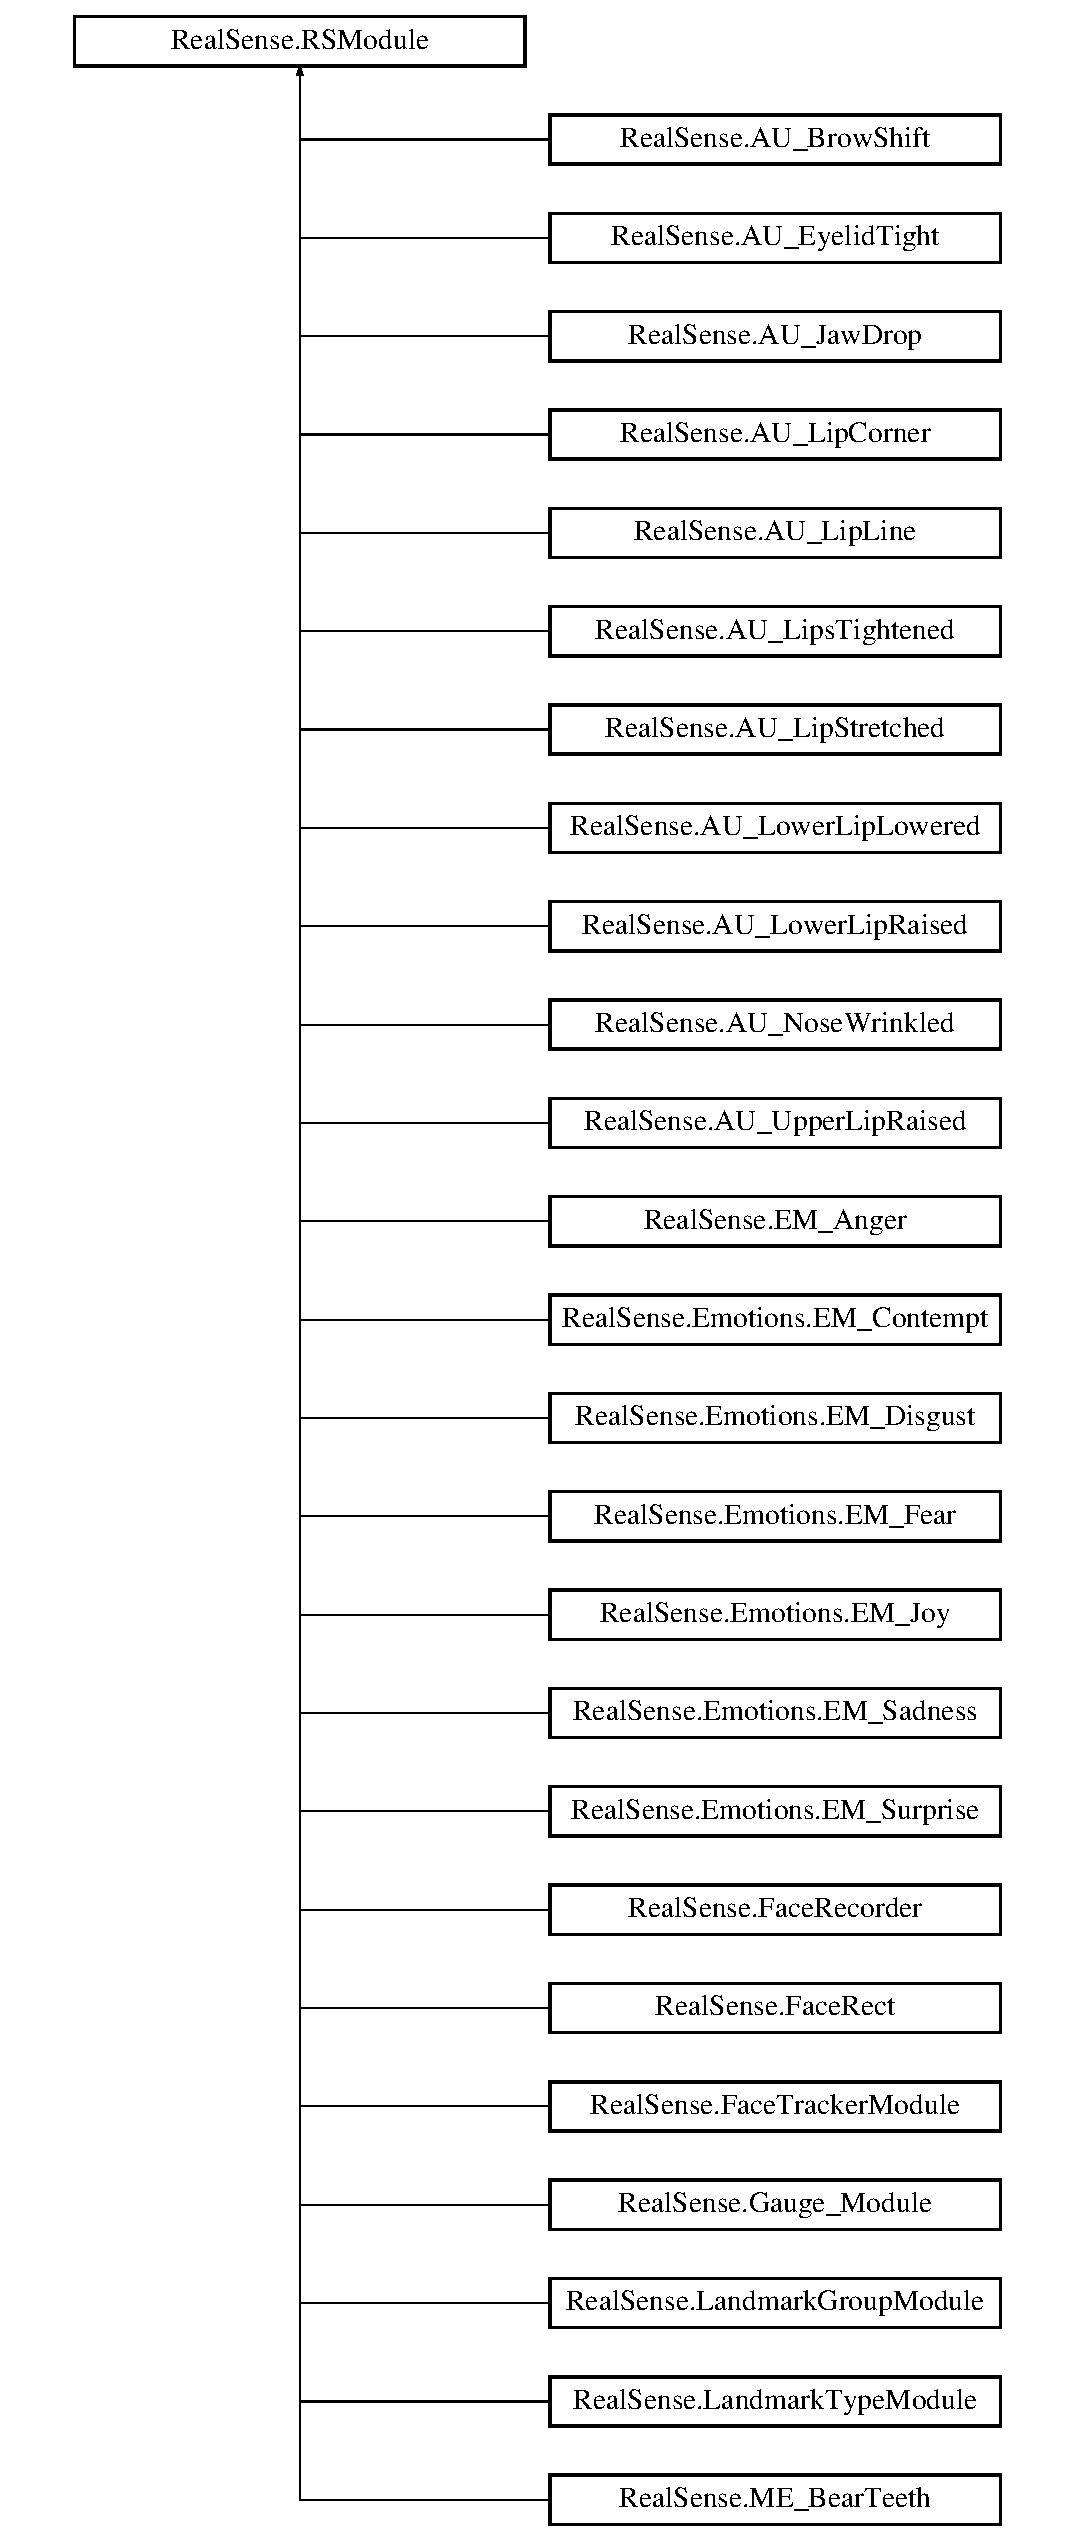
\includegraphics[height=12.000000cm]{class_real_sense_1_1_r_s_module}
\end{center}
\end{figure}
\subsection*{Public Member Functions}
\begin{DoxyCompactItemize}
\item 
virtual void \textbf{ Key\+Trigger} (int key)
\item 
abstract void \textbf{ Work} (Graphics g)
\item 
void \textbf{ Reset} ()
\end{DoxyCompactItemize}
\subsection*{Static Public Member Functions}
\begin{DoxyCompactItemize}
\item 
static void \textbf{ Init} (\textbf{ Model} m)
\end{DoxyCompactItemize}
\subsection*{Public Attributes}
\begin{DoxyCompactItemize}
\item 
String \textbf{ output} = \char`\"{}\char`\"{}
\item 
int [$\,$] \textbf{ triggers} = \{ \}
\end{DoxyCompactItemize}
\subsection*{Protected Member Functions}
\begin{DoxyCompactItemize}
\item 
double [$\,$] \textbf{ Convert\+Values} (double[$\,$] vars)
\item 
double \textbf{ Filtered\+Avg} (double[$\,$] values)
\item 
void \textbf{ Filter\+Tolerance\+Values} (double[$\,$] values)
\item 
void \textbf{ Dynamic\+Min\+Max} (double[$\,$] dist)
\end{DoxyCompactItemize}
\subsection*{Protected Attributes}
\begin{DoxyCompactItemize}
\item 
double \textbf{ M\+IN} = 0
\item 
bool \textbf{ debug} = false
\item 
int \textbf{ frames\+Gathered} = 0
\end{DoxyCompactItemize}
\subsection*{Static Protected Attributes}
\begin{DoxyCompactItemize}
\item 
static double \textbf{ D\+E\+F\+\_\+\+M\+IN}
\item 
static \textbf{ Model} \textbf{ model}
\item 
static int \textbf{ num\+Frames\+Before\+Accept} = 20
\end{DoxyCompactItemize}
\subsection*{Properties}
\begin{DoxyCompactItemize}
\item 
bool \textbf{ Debug}\hspace{0.3cm}{\ttfamily  [get, set]}
\end{DoxyCompactItemize}


\subsection{Detailed Description}
abstract module to implment the Init method of the model and contains the work method

Tanja Witke 

\subsection{Member Function Documentation}
\mbox{\label{class_real_sense_1_1_r_s_module_a53505c9cb3af67e42a0710fdfad65ae5}} 
\index{Real\+Sense\+::\+R\+S\+Module@{Real\+Sense\+::\+R\+S\+Module}!Convert\+Values@{Convert\+Values}}
\index{Convert\+Values@{Convert\+Values}!Real\+Sense\+::\+R\+S\+Module@{Real\+Sense\+::\+R\+S\+Module}}
\subsubsection{Convert\+Values()}
{\footnotesize\ttfamily double [$\,$] Real\+Sense.\+R\+S\+Module.\+Convert\+Values (\begin{DoxyParamCaption}\item[{double [$\,$]}]{vars }\end{DoxyParamCaption})\hspace{0.3cm}{\ttfamily [protected]}}

Resets the Min and the Max value. 
\begin{DoxyParams}{Parameters}
{\em double\mbox{[}$\,$\mbox{]}} & vars -\/ values to consider \\
\hline
\end{DoxyParams}
\begin{DoxyReturn}{Returns}
ret converted values 
\end{DoxyReturn}
\mbox{\label{class_real_sense_1_1_r_s_module_a654263c518b548bad34f5e6ce9c6d2c5}} 
\index{Real\+Sense\+::\+R\+S\+Module@{Real\+Sense\+::\+R\+S\+Module}!Dynamic\+Min\+Max@{Dynamic\+Min\+Max}}
\index{Dynamic\+Min\+Max@{Dynamic\+Min\+Max}!Real\+Sense\+::\+R\+S\+Module@{Real\+Sense\+::\+R\+S\+Module}}
\subsubsection{Dynamic\+Min\+Max()}
{\footnotesize\ttfamily void Real\+Sense.\+R\+S\+Module.\+Dynamic\+Min\+Max (\begin{DoxyParamCaption}\item[{double [$\,$]}]{dist }\end{DoxyParamCaption})\hspace{0.3cm}{\ttfamily [protected]}}

Puts a new Min/\+Max value if the dist is higher/lower than the old one. 
\begin{DoxyParams}{Parameters}
{\em dist} & value to compare \\
\hline
\end{DoxyParams}
\mbox{\label{class_real_sense_1_1_r_s_module_a60d15c600059346aae1effda4a1f9a82}} 
\index{Real\+Sense\+::\+R\+S\+Module@{Real\+Sense\+::\+R\+S\+Module}!Filtered\+Avg@{Filtered\+Avg}}
\index{Filtered\+Avg@{Filtered\+Avg}!Real\+Sense\+::\+R\+S\+Module@{Real\+Sense\+::\+R\+S\+Module}}
\subsubsection{Filtered\+Avg()}
{\footnotesize\ttfamily double Real\+Sense.\+R\+S\+Module.\+Filtered\+Avg (\begin{DoxyParamCaption}\item[{double [$\,$]}]{values }\end{DoxyParamCaption})\hspace{0.3cm}{\ttfamily [protected]}}

Called in Dynamic\+Min\+Max 
\begin{DoxyParams}{Parameters}
{\em double\mbox{[}$\,$\mbox{]}} & vars -\/ values to consider \\
\hline
\end{DoxyParams}
\begin{DoxyReturn}{Returns}
average Average of filtered Values 
\end{DoxyReturn}
\mbox{\label{class_real_sense_1_1_r_s_module_a4294c740efc99c4f5c4034e812f1bdaa}} 
\index{Real\+Sense\+::\+R\+S\+Module@{Real\+Sense\+::\+R\+S\+Module}!Filter\+Tolerance\+Values@{Filter\+Tolerance\+Values}}
\index{Filter\+Tolerance\+Values@{Filter\+Tolerance\+Values}!Real\+Sense\+::\+R\+S\+Module@{Real\+Sense\+::\+R\+S\+Module}}
\subsubsection{Filter\+Tolerance\+Values()}
{\footnotesize\ttfamily void Real\+Sense.\+R\+S\+Module.\+Filter\+Tolerance\+Values (\begin{DoxyParamCaption}\item[{double [$\,$]}]{values }\end{DoxyParamCaption})\hspace{0.3cm}{\ttfamily [protected]}}

Removes values that fall within the tolerance-\/spectrum. 
\begin{DoxyParams}{Parameters}
{\em double\mbox{[}$\,$\mbox{]}} & vars -\/ values to consider \\
\hline
\end{DoxyParams}
\mbox{\label{class_real_sense_1_1_r_s_module_a4a96119975932690f75e86206e1fe63d}} 
\index{Real\+Sense\+::\+R\+S\+Module@{Real\+Sense\+::\+R\+S\+Module}!Init@{Init}}
\index{Init@{Init}!Real\+Sense\+::\+R\+S\+Module@{Real\+Sense\+::\+R\+S\+Module}}
\subsubsection{Init()}
{\footnotesize\ttfamily static void Real\+Sense.\+R\+S\+Module.\+Init (\begin{DoxyParamCaption}\item[{\textbf{ Model}}]{m }\end{DoxyParamCaption})\hspace{0.3cm}{\ttfamily [static]}}

initialise the model 
\begin{DoxyParams}{Parameters}
{\em m} & -\/ the model \\
\hline
\end{DoxyParams}
\mbox{\label{class_real_sense_1_1_r_s_module_a8434d4aa8c289766b24e67cabb7e9471}} 
\index{Real\+Sense\+::\+R\+S\+Module@{Real\+Sense\+::\+R\+S\+Module}!Key\+Trigger@{Key\+Trigger}}
\index{Key\+Trigger@{Key\+Trigger}!Real\+Sense\+::\+R\+S\+Module@{Real\+Sense\+::\+R\+S\+Module}}
\subsubsection{Key\+Trigger()}
{\footnotesize\ttfamily virtual void Real\+Sense.\+R\+S\+Module.\+Key\+Trigger (\begin{DoxyParamCaption}\item[{int}]{key }\end{DoxyParamCaption})\hspace{0.3cm}{\ttfamily [virtual]}}

Custom method when triggered 
\begin{DoxyParams}{Parameters}
{\em int} & key -\/ key to trigger this module \\
\hline
\end{DoxyParams}


Reimplemented in \textbf{ Real\+Sense.\+Face\+Recorder} \doxyref{}{p.}{class_real_sense_1_1_face_recorder_a315985241eb6c21f6393d8104a967eb6}.

\mbox{\label{class_real_sense_1_1_r_s_module_a5dc0fb567c84392f2469f5ed6445b10b}} 
\index{Real\+Sense\+::\+R\+S\+Module@{Real\+Sense\+::\+R\+S\+Module}!Reset@{Reset}}
\index{Reset@{Reset}!Real\+Sense\+::\+R\+S\+Module@{Real\+Sense\+::\+R\+S\+Module}}
\subsubsection{Reset()}
{\footnotesize\ttfamily void Real\+Sense.\+R\+S\+Module.\+Reset (\begin{DoxyParamCaption}{ }\end{DoxyParamCaption})}

Reset value boundaries \mbox{\label{class_real_sense_1_1_r_s_module_a2ec830b7932ee7c0077d473f81c73867}} 
\index{Real\+Sense\+::\+R\+S\+Module@{Real\+Sense\+::\+R\+S\+Module}!Work@{Work}}
\index{Work@{Work}!Real\+Sense\+::\+R\+S\+Module@{Real\+Sense\+::\+R\+S\+Module}}
\subsubsection{Work()}
{\footnotesize\ttfamily abstract void Real\+Sense.\+R\+S\+Module.\+Work (\begin{DoxyParamCaption}\item[{Graphics}]{g }\end{DoxyParamCaption})\hspace{0.3cm}{\ttfamily [pure virtual]}}

Update every frame (do calculations, manipulate output Image) 
\begin{DoxyParams}{Parameters}
{\em Graphics} & g \\
\hline
\end{DoxyParams}


Implemented in \textbf{ Real\+Sense.\+Gauge\+\_\+\+Module} \doxyref{}{p.}{class_real_sense_1_1_gauge___module_a587ea68ad539f2f56bcfbd7641a92a83}, \textbf{ Real\+Sense.\+Face\+Recorder} \doxyref{}{p.}{class_real_sense_1_1_face_recorder_a2adae8c9db76fe9617e99795b4fa5e0e}, \textbf{ Real\+Sense.\+Landmark\+Type\+Module} \doxyref{}{p.}{class_real_sense_1_1_landmark_type_module_ad110598b840e5496c1539862c4c53bc7}, \textbf{ Real\+Sense.\+A\+U\+\_\+\+Eyelid\+Tight} \doxyref{}{p.}{class_real_sense_1_1_a_u___eyelid_tight_a778e09bf84946d959dcf3375a3c8d662}, \textbf{ Real\+Sense.\+A\+U\+\_\+\+Nose\+Wrinkled} \doxyref{}{p.}{class_real_sense_1_1_a_u___nose_wrinkled_afa5099e1c15f8f0f3d9633a42ed69817}, \textbf{ Real\+Sense.\+A\+U\+\_\+\+Brow\+Shift} \doxyref{}{p.}{class_real_sense_1_1_a_u___brow_shift_a81ed7b844c217d3092412e0f53378dd5}, \textbf{ Real\+Sense.\+A\+U\+\_\+\+Lip\+Corner} \doxyref{}{p.}{class_real_sense_1_1_a_u___lip_corner_a4a506c5dc50e7bcd8dcfa80cecbd7f56}, \textbf{ Real\+Sense.\+A\+U\+\_\+\+Lips\+Tightened} \doxyref{}{p.}{class_real_sense_1_1_a_u___lips_tightened_a409b75e75c7b72c628ea6479a50ed75f}, \textbf{ Real\+Sense.\+A\+U\+\_\+\+Lip\+Stretched} \doxyref{}{p.}{class_real_sense_1_1_a_u___lip_stretched_a2ec4542e5c8fa5585e66ee6ee44ab151}, \textbf{ Real\+Sense.\+A\+U\+\_\+\+Lower\+Lip\+Lowered} \doxyref{}{p.}{class_real_sense_1_1_a_u___lower_lip_lowered_ad94e215984e23238a6231d6a9723a522}, \textbf{ Real\+Sense.\+A\+U\+\_\+\+Upper\+Lip\+Raised} \doxyref{}{p.}{class_real_sense_1_1_a_u___upper_lip_raised_a22ea7b3343701718bb2aea731850d81a}, \textbf{ Real\+Sense.\+A\+U\+\_\+\+Jaw\+Drop} \doxyref{}{p.}{class_real_sense_1_1_a_u___jaw_drop_aed90ca88a1c563016c6af39fd65f81e4}, \textbf{ Real\+Sense.\+A\+U\+\_\+\+Lip\+Line} \doxyref{}{p.}{class_real_sense_1_1_a_u___lip_line_ac511da241ef7448f552111e3c5365de1}, \textbf{ Real\+Sense.\+A\+U\+\_\+\+Lower\+Lip\+Raised} \doxyref{}{p.}{class_real_sense_1_1_a_u___lower_lip_raised_aa3949d4b7a3adf5d38cb5ad5acd5c8f2}, \textbf{ Real\+Sense.\+Emotions.\+E\+M\+\_\+\+Contempt} \doxyref{}{p.}{class_real_sense_1_1_emotions_1_1_e_m___contempt_a7ea208f926c1888f028cbe6d6fe14e2f}, \textbf{ Real\+Sense.\+Landmark\+Group\+Module} \doxyref{}{p.}{class_real_sense_1_1_landmark_group_module_aae68525cdcf843719e02fa9b7317d3fa}, \textbf{ Real\+Sense.\+M\+E\+\_\+\+Bear\+Teeth} \doxyref{}{p.}{class_real_sense_1_1_m_e___bear_teeth_a2e4cc340fec3499318fa7514ee7f1822}, \textbf{ Real\+Sense.\+Face\+Tracker\+Module} \doxyref{}{p.}{class_real_sense_1_1_face_tracker_module_a38b7097ab671999aae5f1a645fc623f8}, \textbf{ Real\+Sense.\+E\+M\+\_\+\+Anger} \doxyref{}{p.}{class_real_sense_1_1_e_m___anger_a5c1f3b6b7e84ee926869828a3cfe532a}, \textbf{ Real\+Sense.\+Emotions.\+E\+M\+\_\+\+Joy} \doxyref{}{p.}{class_real_sense_1_1_emotions_1_1_e_m___joy_acce5a4daa0acfd1a10d0aac92ef278c8}, \textbf{ Real\+Sense.\+Emotions.\+E\+M\+\_\+\+Disgust} \doxyref{}{p.}{class_real_sense_1_1_emotions_1_1_e_m___disgust_a22cbe3025c32821d53edcb325140ccb1}, \textbf{ Real\+Sense.\+Emotions.\+E\+M\+\_\+\+Sadness} \doxyref{}{p.}{class_real_sense_1_1_emotions_1_1_e_m___sadness_a45cf23f5c3382bc9769abf1ef401ade1}, \textbf{ Real\+Sense.\+Emotions.\+E\+M\+\_\+\+Fear} \doxyref{}{p.}{class_real_sense_1_1_emotions_1_1_e_m___fear_a5b417a4a8403f101585dc8c239288c54}, \textbf{ Real\+Sense.\+Emotions.\+E\+M\+\_\+\+Surprise} \doxyref{}{p.}{class_real_sense_1_1_emotions_1_1_e_m___surprise_a08040934bb081596a4b02b483dc3a662}, and \textbf{ Real\+Sense.\+Face\+Rect} \doxyref{}{p.}{class_real_sense_1_1_face_rect_aa2dbacb2ec8ac50b8fc19d02ceba2c0a}.



\subsection{Member Data Documentation}
\mbox{\label{class_real_sense_1_1_r_s_module_a5f460d4bb4cb4b000426f9d316deae03}} 
\index{Real\+Sense\+::\+R\+S\+Module@{Real\+Sense\+::\+R\+S\+Module}!debug@{debug}}
\index{debug@{debug}!Real\+Sense\+::\+R\+S\+Module@{Real\+Sense\+::\+R\+S\+Module}}
\subsubsection{debug}
{\footnotesize\ttfamily bool Real\+Sense.\+R\+S\+Module.\+debug = false\hspace{0.3cm}{\ttfamily [protected]}}

\mbox{\label{class_real_sense_1_1_r_s_module_a157703aadbac7416f5fc0eb339546002}} 
\index{Real\+Sense\+::\+R\+S\+Module@{Real\+Sense\+::\+R\+S\+Module}!D\+E\+F\+\_\+\+M\+IN@{D\+E\+F\+\_\+\+M\+IN}}
\index{D\+E\+F\+\_\+\+M\+IN@{D\+E\+F\+\_\+\+M\+IN}!Real\+Sense\+::\+R\+S\+Module@{Real\+Sense\+::\+R\+S\+Module}}
\subsubsection{D\+E\+F\+\_\+\+M\+IN}
{\footnotesize\ttfamily double Real\+Sense.\+R\+S\+Module.\+D\+E\+F\+\_\+\+M\+IN\hspace{0.3cm}{\ttfamily [static]}, {\ttfamily [protected]}}

\mbox{\label{class_real_sense_1_1_r_s_module_aa3ca8a7dcab6b7c9be3021c6d14702cf}} 
\index{Real\+Sense\+::\+R\+S\+Module@{Real\+Sense\+::\+R\+S\+Module}!frames\+Gathered@{frames\+Gathered}}
\index{frames\+Gathered@{frames\+Gathered}!Real\+Sense\+::\+R\+S\+Module@{Real\+Sense\+::\+R\+S\+Module}}
\subsubsection{frames\+Gathered}
{\footnotesize\ttfamily int Real\+Sense.\+R\+S\+Module.\+frames\+Gathered = 0\hspace{0.3cm}{\ttfamily [protected]}}

\mbox{\label{class_real_sense_1_1_r_s_module_aac57c31e50cebecbcb46a0526d7a6ac0}} 
\index{Real\+Sense\+::\+R\+S\+Module@{Real\+Sense\+::\+R\+S\+Module}!M\+IN@{M\+IN}}
\index{M\+IN@{M\+IN}!Real\+Sense\+::\+R\+S\+Module@{Real\+Sense\+::\+R\+S\+Module}}
\subsubsection{M\+IN}
{\footnotesize\ttfamily double Real\+Sense.\+R\+S\+Module.\+M\+IN = 0\hspace{0.3cm}{\ttfamily [protected]}}

\mbox{\label{class_real_sense_1_1_r_s_module_a29ce0491f4813a62b998effa782423d1}} 
\index{Real\+Sense\+::\+R\+S\+Module@{Real\+Sense\+::\+R\+S\+Module}!model@{model}}
\index{model@{model}!Real\+Sense\+::\+R\+S\+Module@{Real\+Sense\+::\+R\+S\+Module}}
\subsubsection{model}
{\footnotesize\ttfamily \textbf{ Model} Real\+Sense.\+R\+S\+Module.\+model\hspace{0.3cm}{\ttfamily [static]}, {\ttfamily [protected]}}

\mbox{\label{class_real_sense_1_1_r_s_module_a9a8c8d17ca9321b558c50f2458a90f3c}} 
\index{Real\+Sense\+::\+R\+S\+Module@{Real\+Sense\+::\+R\+S\+Module}!num\+Frames\+Before\+Accept@{num\+Frames\+Before\+Accept}}
\index{num\+Frames\+Before\+Accept@{num\+Frames\+Before\+Accept}!Real\+Sense\+::\+R\+S\+Module@{Real\+Sense\+::\+R\+S\+Module}}
\subsubsection{num\+Frames\+Before\+Accept}
{\footnotesize\ttfamily int Real\+Sense.\+R\+S\+Module.\+num\+Frames\+Before\+Accept = 20\hspace{0.3cm}{\ttfamily [static]}, {\ttfamily [protected]}}

\mbox{\label{class_real_sense_1_1_r_s_module_a5f0ea0ffd2361fd2b792ed808a67f911}} 
\index{Real\+Sense\+::\+R\+S\+Module@{Real\+Sense\+::\+R\+S\+Module}!output@{output}}
\index{output@{output}!Real\+Sense\+::\+R\+S\+Module@{Real\+Sense\+::\+R\+S\+Module}}
\subsubsection{output}
{\footnotesize\ttfamily String Real\+Sense.\+R\+S\+Module.\+output = \char`\"{}\char`\"{}}

\mbox{\label{class_real_sense_1_1_r_s_module_a100988a1b957067db074dad8b4b9a078}} 
\index{Real\+Sense\+::\+R\+S\+Module@{Real\+Sense\+::\+R\+S\+Module}!triggers@{triggers}}
\index{triggers@{triggers}!Real\+Sense\+::\+R\+S\+Module@{Real\+Sense\+::\+R\+S\+Module}}
\subsubsection{triggers}
{\footnotesize\ttfamily int [$\,$] Real\+Sense.\+R\+S\+Module.\+triggers = \{ \}}



\subsection{Property Documentation}
\mbox{\label{class_real_sense_1_1_r_s_module_a89c9c568ab387b183a63ed2755a82203}} 
\index{Real\+Sense\+::\+R\+S\+Module@{Real\+Sense\+::\+R\+S\+Module}!Debug@{Debug}}
\index{Debug@{Debug}!Real\+Sense\+::\+R\+S\+Module@{Real\+Sense\+::\+R\+S\+Module}}
\subsubsection{Debug}
{\footnotesize\ttfamily bool Real\+Sense.\+R\+S\+Module.\+Debug\hspace{0.3cm}{\ttfamily [get]}, {\ttfamily [set]}}

Getter of the debug value 

The documentation for this class was generated from the following file\+:\begin{DoxyCompactItemize}
\item 
Framework/\textbf{ R\+S\+Module.\+cs}\end{DoxyCompactItemize}

\chapter{File Documentation}
\hypertarget{_a_u___brow_shift_8cs}{}\section{C\+:/\+Users/nutzer/\+Documents/\+Git\+Hub/\+Real\+Sense/\+Action\+Units/\+A\+U\+\_\+\+Brow\+Shift.cs File Reference}
\label{_a_u___brow_shift_8cs}\index{C\+:/\+Users/nutzer/\+Documents/\+Git\+Hub/\+Real\+Sense/\+Action\+Units/\+A\+U\+\_\+\+Brow\+Shift.\+cs@{C\+:/\+Users/nutzer/\+Documents/\+Git\+Hub/\+Real\+Sense/\+Action\+Units/\+A\+U\+\_\+\+Brow\+Shift.\+cs}}
\subsection*{Classes}
\begin{DoxyCompactItemize}
\item 
class \hyperlink{class_real_sense_1_1_a_u___brow_shift}{Real\+Sense.\+A\+U\+\_\+\+Brow\+Shift}
\end{DoxyCompactItemize}
\subsection*{Namespaces}
\begin{DoxyCompactItemize}
\item 
namespace \hyperlink{namespace_real_sense}{Real\+Sense}
\end{DoxyCompactItemize}

\section{Action\+Units/\+A\+U\+\_\+\+Eyelid\+Tight.cs File Reference}
\label{_a_u___eyelid_tight_8cs}\index{Action\+Units/\+A\+U\+\_\+\+Eyelid\+Tight.\+cs@{Action\+Units/\+A\+U\+\_\+\+Eyelid\+Tight.\+cs}}
\subsection*{Classes}
\begin{DoxyCompactItemize}
\item 
class \textbf{ Real\+Sense.\+A\+U\+\_\+\+Eyelid\+Tight}
\end{DoxyCompactItemize}
\subsection*{Namespaces}
\begin{DoxyCompactItemize}
\item 
namespace \textbf{ Real\+Sense}
\end{DoxyCompactItemize}

\section{Action\+Units/\+A\+U\+\_\+\+Jaw\+Drop.cs File Reference}
\label{_a_u___jaw_drop_8cs}\index{Action\+Units/\+A\+U\+\_\+\+Jaw\+Drop.\+cs@{Action\+Units/\+A\+U\+\_\+\+Jaw\+Drop.\+cs}}
\subsection*{Classes}
\begin{DoxyCompactItemize}
\item 
class \textbf{ Real\+Sense.\+A\+U\+\_\+\+Jaw\+Drop}
\end{DoxyCompactItemize}
\subsection*{Namespaces}
\begin{DoxyCompactItemize}
\item 
namespace \textbf{ Real\+Sense}
\end{DoxyCompactItemize}

\hypertarget{_a_u___lip_corner_8cs}{}\section{C\+:/\+Users/nutzer/\+Documents/\+Git\+Hub/\+Real\+Sense/\+Action\+Units/\+A\+U\+\_\+\+Lip\+Corner.cs File Reference}
\label{_a_u___lip_corner_8cs}\index{C\+:/\+Users/nutzer/\+Documents/\+Git\+Hub/\+Real\+Sense/\+Action\+Units/\+A\+U\+\_\+\+Lip\+Corner.\+cs@{C\+:/\+Users/nutzer/\+Documents/\+Git\+Hub/\+Real\+Sense/\+Action\+Units/\+A\+U\+\_\+\+Lip\+Corner.\+cs}}
\subsection*{Classes}
\begin{DoxyCompactItemize}
\item 
class \hyperlink{class_real_sense_1_1_a_u___lip_corner}{Real\+Sense.\+A\+U\+\_\+\+Lip\+Corner}
\end{DoxyCompactItemize}
\subsection*{Namespaces}
\begin{DoxyCompactItemize}
\item 
namespace \hyperlink{namespace_real_sense}{Real\+Sense}
\end{DoxyCompactItemize}

\section{Action\+Units/\+A\+U\+\_\+\+Lip\+Line.cs File Reference}
\label{_a_u___lip_line_8cs}\index{Action\+Units/\+A\+U\+\_\+\+Lip\+Line.\+cs@{Action\+Units/\+A\+U\+\_\+\+Lip\+Line.\+cs}}
\subsection*{Classes}
\begin{DoxyCompactItemize}
\item 
class \textbf{ Real\+Sense.\+A\+U\+\_\+\+Lip\+Line}
\end{DoxyCompactItemize}
\subsection*{Namespaces}
\begin{DoxyCompactItemize}
\item 
namespace \textbf{ Real\+Sense}
\end{DoxyCompactItemize}

\hypertarget{_a_u___lips_tightened_8cs}{}\section{Action\+Units/\+A\+U\+\_\+\+Lips\+Tightened.cs File Reference}
\label{_a_u___lips_tightened_8cs}\index{Action\+Units/\+A\+U\+\_\+\+Lips\+Tightened.\+cs@{Action\+Units/\+A\+U\+\_\+\+Lips\+Tightened.\+cs}}
\subsection*{Classes}
\begin{DoxyCompactItemize}
\item 
class \hyperlink{class_real_sense_1_1_m_e___lips_tightened}{Real\+Sense.\+M\+E\+\_\+\+Lips\+Tightened}
\end{DoxyCompactItemize}
\subsection*{Namespaces}
\begin{DoxyCompactItemize}
\item 
namespace \hyperlink{namespace_real_sense}{Real\+Sense}
\end{DoxyCompactItemize}

\hypertarget{_a_u___lip_stretched_8cs}{}\section{Action\+Units/\+A\+U\+\_\+\+Lip\+Stretched.cs File Reference}
\label{_a_u___lip_stretched_8cs}\index{Action\+Units/\+A\+U\+\_\+\+Lip\+Stretched.\+cs@{Action\+Units/\+A\+U\+\_\+\+Lip\+Stretched.\+cs}}
\subsection*{Classes}
\begin{DoxyCompactItemize}
\item 
class \hyperlink{class_real_sense_1_1_a_u___lip_stretched}{Real\+Sense.\+A\+U\+\_\+\+Lip\+Stretched}
\end{DoxyCompactItemize}
\subsection*{Namespaces}
\begin{DoxyCompactItemize}
\item 
namespace \hyperlink{namespace_real_sense}{Real\+Sense}
\end{DoxyCompactItemize}

\section{Action\+Units/\+A\+U\+\_\+\+Lower\+Lip\+Lowered.cs File Reference}
\label{_a_u___lower_lip_lowered_8cs}\index{Action\+Units/\+A\+U\+\_\+\+Lower\+Lip\+Lowered.\+cs@{Action\+Units/\+A\+U\+\_\+\+Lower\+Lip\+Lowered.\+cs}}
\subsection*{Classes}
\begin{DoxyCompactItemize}
\item 
class \textbf{ Real\+Sense.\+A\+U\+\_\+\+Lower\+Lip\+Lowered}
\end{DoxyCompactItemize}
\subsection*{Namespaces}
\begin{DoxyCompactItemize}
\item 
namespace \textbf{ Real\+Sense}
\end{DoxyCompactItemize}

\hypertarget{_a_u___lower_lip_raised_8cs}{}\section{C\+:/\+Users/nutzer/\+Documents/\+Git\+Hub/\+Real\+Sense/\+Action\+Units/\+A\+U\+\_\+\+Lower\+Lip\+Raised.cs File Reference}
\label{_a_u___lower_lip_raised_8cs}\index{C\+:/\+Users/nutzer/\+Documents/\+Git\+Hub/\+Real\+Sense/\+Action\+Units/\+A\+U\+\_\+\+Lower\+Lip\+Raised.\+cs@{C\+:/\+Users/nutzer/\+Documents/\+Git\+Hub/\+Real\+Sense/\+Action\+Units/\+A\+U\+\_\+\+Lower\+Lip\+Raised.\+cs}}
\subsection*{Classes}
\begin{DoxyCompactItemize}
\item 
class \hyperlink{class_real_sense_1_1_a_u___lower_lip_raised}{Real\+Sense.\+A\+U\+\_\+\+Lower\+Lip\+Raised}
\end{DoxyCompactItemize}
\subsection*{Namespaces}
\begin{DoxyCompactItemize}
\item 
namespace \hyperlink{namespace_real_sense}{Real\+Sense}
\end{DoxyCompactItemize}

\hypertarget{_a_u___nose_wrinkled_8cs}{}\section{Action\+Units/\+A\+U\+\_\+\+Nose\+Wrinkled.cs File Reference}
\label{_a_u___nose_wrinkled_8cs}\index{Action\+Units/\+A\+U\+\_\+\+Nose\+Wrinkled.\+cs@{Action\+Units/\+A\+U\+\_\+\+Nose\+Wrinkled.\+cs}}
\subsection*{Classes}
\begin{DoxyCompactItemize}
\item 
class \hyperlink{class_real_sense_1_1_a_u___nose_wrinkled}{Real\+Sense.\+A\+U\+\_\+\+Nose\+Wrinkled}
\end{DoxyCompactItemize}
\subsection*{Namespaces}
\begin{DoxyCompactItemize}
\item 
namespace \hyperlink{namespace_real_sense}{Real\+Sense}
\end{DoxyCompactItemize}

\section{Action\+Units/\+A\+U\+\_\+\+Upper\+Lip\+Raised.cs File Reference}
\label{_a_u___upper_lip_raised_8cs}\index{Action\+Units/\+A\+U\+\_\+\+Upper\+Lip\+Raised.\+cs@{Action\+Units/\+A\+U\+\_\+\+Upper\+Lip\+Raised.\+cs}}
\subsection*{Classes}
\begin{DoxyCompactItemize}
\item 
class \textbf{ Real\+Sense.\+A\+U\+\_\+\+Upper\+Lip\+Raised}
\end{DoxyCompactItemize}
\subsection*{Namespaces}
\begin{DoxyCompactItemize}
\item 
namespace \textbf{ Real\+Sense}
\end{DoxyCompactItemize}

\hypertarget{_analyzer_view_8cs}{}\section{Analyse/\+Analyzer\+View.cs File Reference}
\label{_analyzer_view_8cs}\index{Analyse/\+Analyzer\+View.\+cs@{Analyse/\+Analyzer\+View.\+cs}}
\subsection*{Classes}
\begin{DoxyCompactItemize}
\item 
class \hyperlink{class_real_sense_1_1_analyzer_view}{Real\+Sense.\+Analyzer\+View}
\end{DoxyCompactItemize}
\subsection*{Namespaces}
\begin{DoxyCompactItemize}
\item 
namespace \hyperlink{namespace_real_sense}{Real\+Sense}
\end{DoxyCompactItemize}

\hypertarget{_face_recorder_8cs}{}\section{C\+:/\+Users/nutzer/\+Documents/\+Git\+Hub/\+Real\+Sense/\+Analyse/\+Face\+Recorder.cs File Reference}
\label{_face_recorder_8cs}\index{C\+:/\+Users/nutzer/\+Documents/\+Git\+Hub/\+Real\+Sense/\+Analyse/\+Face\+Recorder.\+cs@{C\+:/\+Users/nutzer/\+Documents/\+Git\+Hub/\+Real\+Sense/\+Analyse/\+Face\+Recorder.\+cs}}
\subsection*{Classes}
\begin{DoxyCompactItemize}
\item 
class \hyperlink{class_real_sense_1_1_face_recorder}{Real\+Sense.\+Face\+Recorder}
\end{DoxyCompactItemize}
\subsection*{Namespaces}
\begin{DoxyCompactItemize}
\item 
namespace \hyperlink{namespace_real_sense}{Real\+Sense}
\end{DoxyCompactItemize}

\hypertarget{_face_recording_8cs}{}\section{Analyse/\+Face\+Recording.cs File Reference}
\label{_face_recording_8cs}\index{Analyse/\+Face\+Recording.\+cs@{Analyse/\+Face\+Recording.\+cs}}
\subsection*{Classes}
\begin{DoxyCompactItemize}
\item 
class \hyperlink{class_real_sense_1_1_face_recording}{Real\+Sense.\+Face\+Recording}
\end{DoxyCompactItemize}
\subsection*{Namespaces}
\begin{DoxyCompactItemize}
\item 
namespace \hyperlink{namespace_real_sense}{Real\+Sense}
\end{DoxyCompactItemize}

\section{Emotions/\+Assembly\+Info.cs File Reference}
\label{_assembly_info_8cs}\index{Emotions/\+Assembly\+Info.\+cs@{Emotions/\+Assembly\+Info.\+cs}}

\hypertarget{_e_m___anger_8cs}{}\section{Emotions/\+E\+M\+\_\+\+Anger.cs File Reference}
\label{_e_m___anger_8cs}\index{Emotions/\+E\+M\+\_\+\+Anger.\+cs@{Emotions/\+E\+M\+\_\+\+Anger.\+cs}}
\subsection*{Classes}
\begin{DoxyCompactItemize}
\item 
class \hyperlink{class_real_sense_1_1_e_m___anger}{Real\+Sense.\+E\+M\+\_\+\+Anger}
\end{DoxyCompactItemize}
\subsection*{Namespaces}
\begin{DoxyCompactItemize}
\item 
namespace \hyperlink{namespace_real_sense}{Real\+Sense}
\end{DoxyCompactItemize}

\section{Emotions/\+E\+M\+\_\+\+Contempt.cs File Reference}
\label{_e_m___contempt_8cs}\index{Emotions/\+E\+M\+\_\+\+Contempt.\+cs@{Emotions/\+E\+M\+\_\+\+Contempt.\+cs}}
\subsection*{Classes}
\begin{DoxyCompactItemize}
\item 
class \textbf{ Real\+Sense.\+Emotions.\+E\+M\+\_\+\+Contempt}
\end{DoxyCompactItemize}
\subsection*{Namespaces}
\begin{DoxyCompactItemize}
\item 
namespace \textbf{ Real\+Sense.\+Emotions}
\end{DoxyCompactItemize}

\section{Emotions/\+E\+M\+\_\+\+Disgust.cs File Reference}
\label{_e_m___disgust_8cs}\index{Emotions/\+E\+M\+\_\+\+Disgust.\+cs@{Emotions/\+E\+M\+\_\+\+Disgust.\+cs}}
\subsection*{Classes}
\begin{DoxyCompactItemize}
\item 
class \textbf{ Real\+Sense.\+Emotions.\+E\+M\+\_\+\+Disgust}
\end{DoxyCompactItemize}
\subsection*{Namespaces}
\begin{DoxyCompactItemize}
\item 
namespace \textbf{ Real\+Sense.\+Emotions}
\end{DoxyCompactItemize}

\hypertarget{_e_m___fear_8cs}{}\section{C\+:/\+Users/nutzer/\+Documents/\+Git\+Hub/\+Real\+Sense/\+Emotions/\+E\+M\+\_\+\+Fear.cs File Reference}
\label{_e_m___fear_8cs}\index{C\+:/\+Users/nutzer/\+Documents/\+Git\+Hub/\+Real\+Sense/\+Emotions/\+E\+M\+\_\+\+Fear.\+cs@{C\+:/\+Users/nutzer/\+Documents/\+Git\+Hub/\+Real\+Sense/\+Emotions/\+E\+M\+\_\+\+Fear.\+cs}}
\subsection*{Classes}
\begin{DoxyCompactItemize}
\item 
class \hyperlink{class_real_sense_1_1_emotions_1_1_e_m___fear}{Real\+Sense.\+Emotions.\+E\+M\+\_\+\+Fear}
\end{DoxyCompactItemize}
\subsection*{Namespaces}
\begin{DoxyCompactItemize}
\item 
namespace \hyperlink{namespace_real_sense_1_1_emotions}{Real\+Sense.\+Emotions}
\end{DoxyCompactItemize}

\hypertarget{_e_m___joy_8cs}{}\section{Emotions/\+E\+M\+\_\+\+Joy.cs File Reference}
\label{_e_m___joy_8cs}\index{Emotions/\+E\+M\+\_\+\+Joy.\+cs@{Emotions/\+E\+M\+\_\+\+Joy.\+cs}}
\subsection*{Classes}
\begin{DoxyCompactItemize}
\item 
class \hyperlink{class_real_sense_1_1_emotions_1_1_e_m___joy}{Real\+Sense.\+Emotions.\+E\+M\+\_\+\+Joy}
\end{DoxyCompactItemize}
\subsection*{Namespaces}
\begin{DoxyCompactItemize}
\item 
namespace \hyperlink{namespace_real_sense_1_1_emotions}{Real\+Sense.\+Emotions}
\end{DoxyCompactItemize}

\hypertarget{_e_m___sadness_8cs}{}\section{Emotions/\+E\+M\+\_\+\+Sadness.cs File Reference}
\label{_e_m___sadness_8cs}\index{Emotions/\+E\+M\+\_\+\+Sadness.\+cs@{Emotions/\+E\+M\+\_\+\+Sadness.\+cs}}
\subsection*{Classes}
\begin{DoxyCompactItemize}
\item 
class \hyperlink{class_real_sense_1_1_emotions_1_1_e_m___sadness}{Real\+Sense.\+Emotions.\+E\+M\+\_\+\+Sadness}
\end{DoxyCompactItemize}
\subsection*{Namespaces}
\begin{DoxyCompactItemize}
\item 
namespace \hyperlink{namespace_real_sense_1_1_emotions}{Real\+Sense.\+Emotions}
\end{DoxyCompactItemize}

\hypertarget{_e_m___surprise_8cs}{}\section{Emotions/\+E\+M\+\_\+\+Surprise.cs File Reference}
\label{_e_m___surprise_8cs}\index{Emotions/\+E\+M\+\_\+\+Surprise.\+cs@{Emotions/\+E\+M\+\_\+\+Surprise.\+cs}}
\subsection*{Classes}
\begin{DoxyCompactItemize}
\item 
class \hyperlink{class_real_sense_1_1_emotions_1_1_e_m___surprise}{Real\+Sense.\+Emotions.\+E\+M\+\_\+\+Surprise}
\end{DoxyCompactItemize}
\subsection*{Namespaces}
\begin{DoxyCompactItemize}
\item 
namespace \hyperlink{namespace_real_sense_1_1_emotions}{Real\+Sense.\+Emotions}
\end{DoxyCompactItemize}

\hypertarget{_camera_view_8cs}{}\section{C\+:/\+Users/nutzer/\+Documents/\+Git\+Hub/\+Real\+Sense/\+Framework/\+Camera\+View.cs File Reference}
\label{_camera_view_8cs}\index{C\+:/\+Users/nutzer/\+Documents/\+Git\+Hub/\+Real\+Sense/\+Framework/\+Camera\+View.\+cs@{C\+:/\+Users/nutzer/\+Documents/\+Git\+Hub/\+Real\+Sense/\+Framework/\+Camera\+View.\+cs}}
\subsection*{Classes}
\begin{DoxyCompactItemize}
\item 
class \hyperlink{class_real_sense_1_1_camera_view}{Real\+Sense.\+Camera\+View}
\end{DoxyCompactItemize}
\subsection*{Namespaces}
\begin{DoxyCompactItemize}
\item 
namespace \hyperlink{namespace_real_sense}{Real\+Sense}
\end{DoxyCompactItemize}

\hypertarget{_friggn_aweseome_graphix_8cs}{}\section{C\+:/\+Users/nutzer/\+Documents/\+Git\+Hub/\+Real\+Sense/\+Framework/\+Friggn\+Aweseome\+Graphix.cs File Reference}
\label{_friggn_aweseome_graphix_8cs}\index{C\+:/\+Users/nutzer/\+Documents/\+Git\+Hub/\+Real\+Sense/\+Framework/\+Friggn\+Aweseome\+Graphix.\+cs@{C\+:/\+Users/nutzer/\+Documents/\+Git\+Hub/\+Real\+Sense/\+Framework/\+Friggn\+Aweseome\+Graphix.\+cs}}
\subsection*{Classes}
\begin{DoxyCompactItemize}
\item 
class \hyperlink{class_real_sense_1_1_friggn_aweseome_graphix}{Real\+Sense.\+Friggn\+Aweseome\+Graphix}
\item 
class \hyperlink{class_real_sense_1_1_friggn_aweseome_graphix_1_1_m_e_monitor}{Real\+Sense.\+Friggn\+Aweseome\+Graphix.\+M\+E\+Monitor}
\end{DoxyCompactItemize}
\subsection*{Namespaces}
\begin{DoxyCompactItemize}
\item 
namespace \hyperlink{namespace_real_sense}{Real\+Sense}
\end{DoxyCompactItemize}

\section{Framework/\+Model.cs File Reference}
\label{_model_8cs}\index{Framework/\+Model.\+cs@{Framework/\+Model.\+cs}}
\subsection*{Classes}
\begin{DoxyCompactItemize}
\item 
class \textbf{ Real\+Sense.\+Model}
\end{DoxyCompactItemize}
\subsection*{Namespaces}
\begin{DoxyCompactItemize}
\item 
namespace \textbf{ Real\+Sense}
\end{DoxyCompactItemize}

\section{Framework/\+R\+S\+Module.cs File Reference}
\label{_r_s_module_8cs}\index{Framework/\+R\+S\+Module.\+cs@{Framework/\+R\+S\+Module.\+cs}}
\subsection*{Classes}
\begin{DoxyCompactItemize}
\item 
class \textbf{ Real\+Sense.\+R\+S\+Module}
\end{DoxyCompactItemize}
\subsection*{Namespaces}
\begin{DoxyCompactItemize}
\item 
namespace \textbf{ Real\+Sense}
\end{DoxyCompactItemize}

\hypertarget{_program_8cs}{}\section{C\+:/\+Users/nutzer/\+Documents/\+Git\+Hub/\+Real\+Sense/\+Program.cs File Reference}
\label{_program_8cs}\index{C\+:/\+Users/nutzer/\+Documents/\+Git\+Hub/\+Real\+Sense/\+Program.\+cs@{C\+:/\+Users/nutzer/\+Documents/\+Git\+Hub/\+Real\+Sense/\+Program.\+cs}}
\subsection*{Classes}
\begin{DoxyCompactItemize}
\item 
class \hyperlink{class_real_sense_1_1_program}{Real\+Sense.\+Program}
\end{DoxyCompactItemize}
\subsection*{Namespaces}
\begin{DoxyCompactItemize}
\item 
namespace \hyperlink{namespace_real_sense}{Real\+Sense}
\end{DoxyCompactItemize}

\section{Properties/\+Resources.Designer.\+cs File Reference}
\label{_resources_8_designer_8cs}\index{Properties/\+Resources.\+Designer.\+cs@{Properties/\+Resources.\+Designer.\+cs}}
\subsection*{Classes}
\begin{DoxyCompactItemize}
\item 
class {\bfseries Real\+Sense.\+Properties.\+Resources}
\begin{DoxyCompactList}\small\item\em A strongly-\/typed resource class, for looking up localized strings, etc. \end{DoxyCompactList}\end{DoxyCompactItemize}
\subsection*{Namespaces}
\begin{DoxyCompactItemize}
\item 
namespace \textbf{ Real\+Sense.\+Properties}
\end{DoxyCompactItemize}

\section{Various/\+Face\+Rect.cs File Reference}
\label{_face_rect_8cs}\index{Various/\+Face\+Rect.\+cs@{Various/\+Face\+Rect.\+cs}}
\subsection*{Classes}
\begin{DoxyCompactItemize}
\item 
class \textbf{ Real\+Sense.\+Face\+Rect}
\end{DoxyCompactItemize}
\subsection*{Namespaces}
\begin{DoxyCompactItemize}
\item 
namespace \textbf{ Real\+Sense}
\end{DoxyCompactItemize}

\hypertarget{_face_tracker_module_8cs}{}\section{C\+:/\+Users/nutzer/\+Documents/\+Git\+Hub/\+Real\+Sense/\+Various/\+Face\+Tracker\+Module.cs File Reference}
\label{_face_tracker_module_8cs}\index{C\+:/\+Users/nutzer/\+Documents/\+Git\+Hub/\+Real\+Sense/\+Various/\+Face\+Tracker\+Module.\+cs@{C\+:/\+Users/nutzer/\+Documents/\+Git\+Hub/\+Real\+Sense/\+Various/\+Face\+Tracker\+Module.\+cs}}
\subsection*{Classes}
\begin{DoxyCompactItemize}
\item 
class \hyperlink{class_real_sense_1_1_face_tracker_module}{Real\+Sense.\+Face\+Tracker\+Module}
\end{DoxyCompactItemize}
\subsection*{Namespaces}
\begin{DoxyCompactItemize}
\item 
namespace \hyperlink{namespace_real_sense}{Real\+Sense}
\end{DoxyCompactItemize}

\section{Various/\+Gauge\+\_\+\+Module.cs File Reference}
\label{_gauge___module_8cs}\index{Various/\+Gauge\+\_\+\+Module.\+cs@{Various/\+Gauge\+\_\+\+Module.\+cs}}
\subsection*{Classes}
\begin{DoxyCompactItemize}
\item 
class \textbf{ Real\+Sense.\+Gauge\+\_\+\+Module}
\end{DoxyCompactItemize}
\subsection*{Namespaces}
\begin{DoxyCompactItemize}
\item 
namespace \textbf{ Real\+Sense}
\end{DoxyCompactItemize}

\hypertarget{_landmark_group_module_8cs}{}\section{Various/\+Landmark\+Group\+Module.cs File Reference}
\label{_landmark_group_module_8cs}\index{Various/\+Landmark\+Group\+Module.\+cs@{Various/\+Landmark\+Group\+Module.\+cs}}
\subsection*{Classes}
\begin{DoxyCompactItemize}
\item 
class \hyperlink{class_real_sense_1_1_landmark_group_module}{Real\+Sense.\+Landmark\+Group\+Module}
\end{DoxyCompactItemize}
\subsection*{Namespaces}
\begin{DoxyCompactItemize}
\item 
namespace \hyperlink{namespace_real_sense}{Real\+Sense}
\end{DoxyCompactItemize}

\section{Various/\+Landmark\+Type\+Module.cs File Reference}
\label{_landmark_type_module_8cs}\index{Various/\+Landmark\+Type\+Module.\+cs@{Various/\+Landmark\+Type\+Module.\+cs}}
\subsection*{Classes}
\begin{DoxyCompactItemize}
\item 
class \textbf{ Real\+Sense.\+Landmark\+Type\+Module}
\end{DoxyCompactItemize}
\subsection*{Namespaces}
\begin{DoxyCompactItemize}
\item 
namespace \textbf{ Real\+Sense}
\end{DoxyCompactItemize}

\section{Various/\+M\+E\+\_\+\+Bear\+Teeth.cs File Reference}
\label{_m_e___bear_teeth_8cs}\index{Various/\+M\+E\+\_\+\+Bear\+Teeth.\+cs@{Various/\+M\+E\+\_\+\+Bear\+Teeth.\+cs}}
\subsection*{Classes}
\begin{DoxyCompactItemize}
\item 
class \textbf{ Real\+Sense.\+M\+E\+\_\+\+Bear\+Teeth}
\end{DoxyCompactItemize}
\subsection*{Namespaces}
\begin{DoxyCompactItemize}
\item 
namespace \textbf{ Real\+Sense}
\end{DoxyCompactItemize}

%--- End generated contents ---

% Index
\backmatter
\newpage
\phantomsection
\clearemptydoublepage
\addcontentsline{toc}{chapter}{Index}
\printindex

\end{document}
